%% File encoding: UTF-8
%% äöüÄÖÜß  <-- keine deutschen Umlaute hier? UTF-faehigen Editor verwenden!

\documentclass[master,english]{hgbthesis}
% Zulässige Class Options: 
%   Typ der Arbeit: diplom, master (default), bachelor, praktikum 
%   Hauptsprache: german (default), english
%%------------------------------------------------------------

\RequirePackage[utf8]{inputenc}		% remove when using lualatex oder xelatex!

\graphicspath{{images/}}    % name of directory containing the images
\logofile{logo}							% name of logo-PDF in images/ (or use \logofile{} for no logo)
\bibliography{literature}  	% name of the BibTeX (.bib) file


%%%----------------------------------------------------------
\begin{document}
%%%----------------------------------------------------------

% Einträge für ALLE Arbeiten: --------------------------------
\title{Mobile Device Usage in Interactive, Co-located Presentations}
\author{Iris M.\ Schaffer}
\studiengang{Interactive Media}
\studienort{Hagenberg}
\abgabedatum{2016}{09}{26}	% {YYYY}{MM}{DD}

%%%----------------------------------------------------------
\frontmatter
\maketitle
\tableofcontents
%%%----------------------------------------------------------

\chapter{Acknowledgments}
At this point, I would like to express my gratitude to everyone who has joined me on the venture of my masters degree, may it be actively or passively. Those who offered advice and guidance when in doubt, those who motivated and inspired me to always strive for more and those who listened to me and let me spark their interest. In particular, my thank goes to my parents who have always supported me in whatever it was I set my mind on, both financially and with advice. My friends, for both sitting me down in front of my computer when I lost motivation and for taking my mind off work when sinking into it too deeply. Special thanks to Leandro Ostera and his enthusiasm, for lifting my spirits, but also for all the theoretical as well as practical advice and involvement in this project.

Moreover, I want to express my gratitude to my supervisor Dr. Michael Haller for providing me with ideas, feedback and the necessary flexibility to write this thesis remotely, from Sweden. On this note, I want to also thank Oakwood Creative AB for supporting their employee's dreams and visions and for giving me the possibility to test the developed system in meetings as well as Monday morning presentations. Thanks also to my colleagues, for their constant feedback and patience with my Swedish, as well as to every last stranger, in Sweden, Austria and elsewhere, I had the pleasure of telling about my research.

Finally, my admiration and appreciation go out to all developers and companies driving the course of open-source forward. Despite mostly not scientifically publishing their results, this community has given birth to some of the most exciting and most widely used technologies, libraries and frameworks on the market. Without the work of these never-resting individuals, this thesis and project would never have come into existence in their current form. To pay tribute to this vibrant community, all the work involved in this thesis was also open-sourced and published on GitHub\footnote{\href{https://github.com/irisSchaffer?tab=repositories}{\textsf{https://github.com/irisSchaffer/}}}.
\chapter{Abstract}
Mobile devices such as smartphones, tablets and laptops have become our every day companions and can act as an endless source of information, knowledge and inspiration. However, despite studies having demonstrated the benefits of targeted smartphone use in classrooms and meetings, they are still perceived as impolite and disturbing during presentations. These, on the other hand, are often still one-man endeavours, from slide preparation, giving the talk to lastly follow-up work such as hand-outs. In an effort to destigmatise mobile devices usage and make presentations more memorable, engaging, and collaborative, a prototype of an extensible JavaScript presentation eco\-system with a multitude of interactive mechanisms was implemented. These functionalities are the result of the analysis of several types of presentations and their weaknesses and, amongst others, include the possibility for the audience to browse and follow slides on any mobile device to account for individual learning-pace, as well as spontaneous reactions via emoji and votes on polls (both prepared and created on-the-fly) to more reliably estimate ones crowd's mood and background knowledge. Moreover, to truely involve audience memers in shaping the presentation, the functionality to alter the $2$-dimensional slide-sets in real time was realised. This way, listeners can share related multi-media content as well as questions and comments as new main or sub-slides.

Although more thorough, long-term studies will be necessary to validate our approach, consequent informal evaluation of the system in internal presentations and meetings has been promising and decidedly positive. Despite showing room for improvement, all features were understood by the users, with the content sharing functionality sparking most interest and excitement among listeners. The observation of the usage of the tool has moreover given way to further research projects and ideas. 			

\chapter{Kurzfassung}

An dieser Stelle steht eine Zusammenfassung der Arbeit, Umfang
max.\ 1 Seite. Im Unterschied zu anderen Kapiteln ist die
Kurzfassung (und das Abstract) üblicherweise nicht in Abschnitte
und Unterabschnitte gegliedert. 
Auch Fußnoten sind hier falsch am Platz.

Kurzfassungen werden übrigens häufig -- zusammen mit Autor und Titel
der Arbeit -- %
in Literaturdatenbanken aufgenommen. Es ist daher darauf zu
achten, dass die Information in der Kurzfassung für sich 
\emph{allein} (\dah ohne weitere Teile der Arbeit) zusammenhängend und
abgeschlossen ist. Insbesondere werden an dieser Stelle (wie \ua
auch im \emph{Titel} der Arbeit und im \emph{Abstract})
normalerweise \emph{keine Literaturverweise} verwendet! Falls
unbedingt solche benötigt werden -- etwa weil die Arbeit eine
Weiterentwicklung einer bestimmten, früheren Arbeit darstellt --,
dann sind \emph{vollständige} Quellenangaben in der Kurzfassung
selbst notwendig, \zB %
[\textsc{Zobel} J.: \textit{Writing for Computer Science -- The Art of
Effective Commu\-nica\-tion}. Springer-Verlag, Singa\-pur, 1997].

Weiters sollte daran gedacht werden, dass bei der Aufnahme in Datenbanken
Sonderzeichen oder etwa Aufzählungen mit "`Knödellisten"' in der
Regel verloren gehen. Dasselbe gilt natürlich auch für das 
\emph{Abstract}.


Inhaltlich sollte die Kurzfassung \emph{keine} Auflistung der
einzelnen Kapitel sein (dafür ist das Einleitungskapitel
vorgesehen), sondern dem Leser einen kompakten, inhaltlichen
Überblick über die gesamte Arbeit verschaffen. Der hier verwendete
Aufbau ist daher zwangsläufig anders als der in der Einleitung.
		
%

%%%----------------------------------------------------------
\mainmatter         % Hauptteil (ab hier arab. Seitenzahlen)
%%%----------------------------------------------------------

\chapter{Introduction}
\label{cha:introduction}

\section{Motivation}

Mobile phones, tablets and laptops have become our every day companions. We take them with us wherever we go, may it be the classroom or meetings, lately they have even made an appearance in courtrooms \cite{Farrell:TrialByTablet}. Especially during presentations mobile device usage is still perceived as impolite and can be a source of distraction \cite{Bohmer:SmartphoneUseRude, Bajko:ComparativePerceptionSmartphoneMeeting, Kuznekoff:ImpactPhoneStudentLearning}, although studies indicate that lecture-relevant phone use in classrooms can actually be beneficial for information-recall \cite{Kuznekoff:MobilePhoneClassroomTwitter}.

Presentations, on the other hand, have remained largely unchanged since the launch of PowerPoint in the late 1980s \cite{Yates:PowerPoint}. In fact, some of the features overhead projectors innately offered, namely the annotation of transparencies during the presentation and sorting and choosing slides before presenting them, have effectively been lost with the introduction of presentation software. While the amount of presentations given has continuously risen, the modus of presenting has stayed untouched: In most cases, there is one presenter and a group of co-located listeners. The speaker prepares slides prior to a presentation and has the responsibility of educating, fascinating, inspiring and keeping the audience awake, while catering the presented contents to the respective listeners. Although interactive elements in presentations have proven to be twice as effective at engaging listeners and beneficial to information-recall \cite{prezi-science}, presentations have largely remained a static endeavor for the speaker alone.

Mobile phones, tablets and laptops, however, hold the potential of challenging this status quo. Their growing computing power as well as ubiquitousness make them suitable candidates for interacting with presentation software, thus transforming presentations into a more collaborative effort. Instead of banning modern technologies, incorporating mobile devices has proven to foster collaboration and connection between attendees in meetings \cite{Bohmer:SmartphoneUseRude} and has the potential of promoting participation and helping introverts overcome the hurdle of speaking out loud \cite{Bry:Backstage}. At the core of this thesis therefore stands the question: How can mobile devices be integrated into presentation workflows to engage and involve the audience, while transforming the stigma around mobile phones into something positive?

\section{Goals}

\begin{figure}
\centering
\includegraphics[width=.8\textwidth]{illustrations/meeting}
\caption{Unveil presentation in action: the projector displays the current slide, listeners can follow and interact with presentations on their personal devices and listeners can control the presentation using theirs.}
\label{fig:introduction-meeting}
\end{figure}

The main objective of the project consequently is the exploration of different ways of incorporating personal devices in presentations efficiently and productively. This involves both the conception of such mechanisms, as well as their implementation in an online presentation tool.
Due to the high number of different settings and contexts in which talks can be given, and since we feel meetings and other business-related presentations with small numbers of attendees offer the perfect playground and most possibilities for interactive mechanisms, this thesis focuses on presentations in business-settings.

The proposed presentation software includes device-independent altering of pre-defined $2$-dimensional slide-sets by listeners and presenters in real time. It allows audience members to view slides on their personal devices, either navigating freely or synchronised with the presenter (see figure \ref{fig:introduction-meeting}). Additionally, the developed libraries offer support for real-time voting, as well as voting creation on-the-fly. Instantaneous audience reactions via emoji and different paths through the presentation were also realised.

As far as the implementation is concerned, it was our declared goal to create a modular ecosystem other developers can tap into, reuse, overwrite and extend. Since the web was chosen as a platform for its rapid prototyping and iteration cylce possibilities, it was paramount to make the application feel as fast and responsive as possible, to give it the look and feel of a native application \cite{Charland:WebVsNative}. Therefore the user interface and interaction design were at the core of the project with the overall objective of creating an interface that works across all devices, without feeling unnatural.

Finally, an evaluation of the developed mechanisms was desirable. Since thorough long-term studies with control groups are beyond the scope of a master thesis, we constrained ourselves to the informal observation of the system in a series of internal meetings and presentations.

\section{Structure}

This thesis is organised into eight main chapters. First of all, we want to establish the context around the present work by introducing the reader to existing research and projects in the field of interactive presentations in chapter \ref{cha:related-work}. Since an overwhelming number of studies have been conducted in educational settings, the chapter is further divided into classroom \ref{sec:related-work-classroom} and office \ref{sec:related-work-office} related approaches as well as general presentations \ref{sec:related-work-general}.

In chapter \ref{cha:mechanisms} different types of presentations are analysed for their shortcomings and suitable solutions are developed. These are formulated into distinct interactive mechanisms for which clear requirements are established.
Based on these requirements, chapter \ref{cha:design} goes into details on the interface and interaction design of the application as a whole and each of its interactive mechanisms. The general flow and setup of the proposed software are also discussed.

Chapter \ref{cha:implementation} lays out the entire implementation of the libraries involved in the presentation tool. It first defines the scope of the project \ref{sec:implementation-scope} to then cover the server setup \ref{sec:implementation-server}, before offering more insight into the underlying front end technologies used \ref{sec:implementation-technologies}. Finally the general project structure \ref{sec:implementation-structure}, as well as all developed libraries are discussed in detail.

Since we pride ourselves in having developed an entirely open-sourced presentation ecosystem which we want others to explore, reuse and extend, chapter \ref{cha:results} shortly addresses the usage of the resulting libraries from a developer's perspective.

Chapter \ref{cha:discussion} outlines the results of our informal evaluation and observation of the system in regards to its usability \ref{sec:discussion-usability} and the creation of presentations \ref{sec:discussion-dev}, to then reflect on the chosen architecture \ref{sec:discussion-architecture} and give an outlook on future work \ref{sec:discussion-future-work}.

Finally, we briefly talk about the conclusions we draw from this project in chapter \ref{cha:conclusion} and again summarise our findings.
\chapter{Related Work}
\label{cha:related-work}

Mobile phones, tablets and laptops have become our every day companions. We take them with us wherever we go, may it be the classroom or meetings, lately they have even made an appearance in courtrooms \cite{Farrell:TrialByTablet}. Especially during presentations, mobile device usage is still perceived as rude and can be a source of distraction \cite{Bohmer:SmartphoneUseRude, Bajko:ComparativePerceptionSmartphoneMeeting, Kuznekoff:ImpactPhoneStudentLearning} although other studies indicate that lecture-relevant phone use in classrooms can actually be beneficial \cite{Kuznekoff:MobilePhoneClassroomTwitter} for information-recall.

Instead of banning modern technologies, incorporating mobile devices into presentation workflows has proven to foster collaboration and connection between attendees in meetings \cite{Bohmer:SmartphoneUseRude} and holds the potential of promoting participation and helping introverts overcome the hurdle of speaking out loud \cite{Bry:Backstage}. The growing computing power as well as the ubiquitousness of mobile phones, tablets and laptops make them suitable candidates for giving instant feedback to speakers as well as voting and sharing relevant multi-media content on-the-fly. Resulting presentations provide more flexibility, a better understanding of the listeners' opinion and the possibility to close the gap between presenter and audience.

The idea of using electronic devices to foster group interaction in meetings and presentations is not new. Stefik et al. \cite{Stefik:BeyondTheChalkboard} already experimented with the use of personal computers in meeting rooms as early as 1987 and Myers et al. \cite{Myers:CollaborationPDAs} developed a collaboration tool which could be used to annotate PowerPoint slides from PDAs in 1998. Since then, digital whiteboards, telepresence systems, productive multi-user web applications and other computer-aided collaboration tools have become a common sight and we choose to carry smart devices around wherever we go. Surprisingly little research, however, has covered the use of these mobile devices in the context of presentations. Most of these studies were conducted in the educational sector and usually aim at quizzing students, which is why an own sub section is dedicated to classroom related approaches. 

\section{Classroom related}

\begin{figure}
\centering
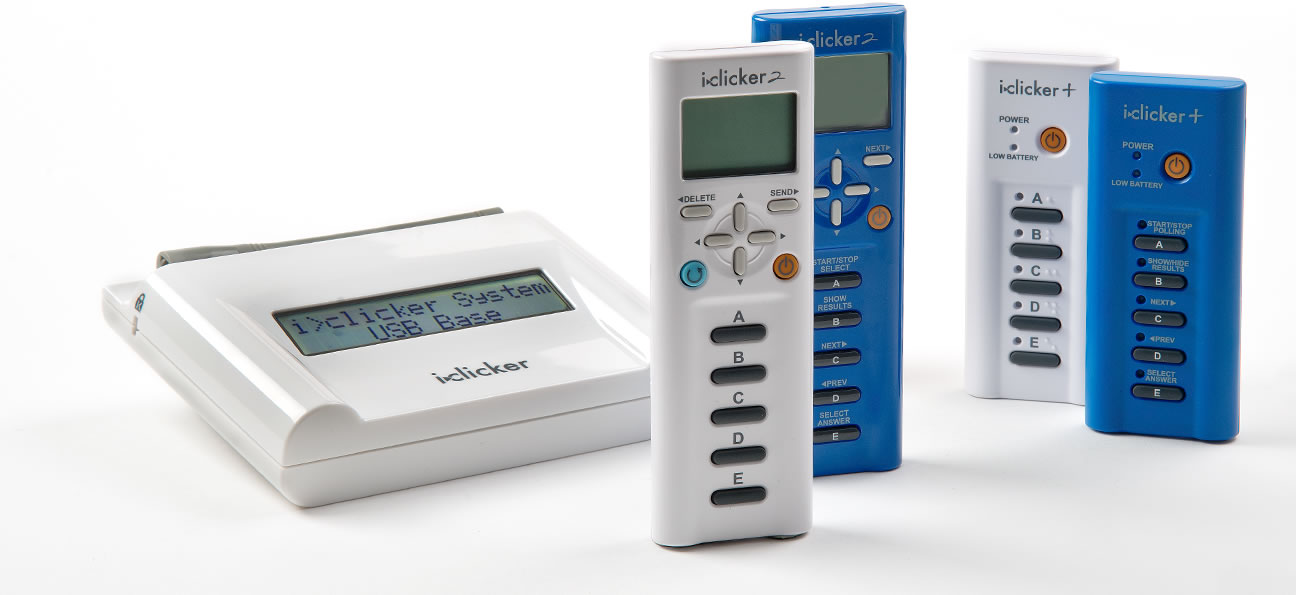
\includegraphics[width=.65\textwidth]{iclickers}
\caption{\emph{i>clicker} devices, used in \cite{Chamillard:StudentResponseSystem}. Image source \cite{iclicker}.}
\label{fig:related-work-iclicker}
\end{figure}

As growing class-sizes have caused student participation to sink drastically \cite{Bry:Backstage}, researchers have tried to deploy mechanisms to make lectures more interactive and engaging. The first ap\-proa\-ches in this field of student-response-systems (SRS) utilised so-called clickers (see figure \ref{fig:related-work-iclicker}) -- remote-control-like devices, connected to a receiver station via radio frequency technology \cite{cuclickers:faq} which can be used for tasks like taking attendance and voting \cite{Chamillard:StudentResponseSystem}. Using these clicker systems has shown to ``yield a strong and positive relationship with student learning'' \cite{Chamillard:StudentResponseSystem}. However, the limitations of clickers -- the need for proprietary hardware and the limited interface consisting only of a few buttons -- lead researchers to experiment with personal mobile devices as input instead. In 2007 Lindquist et al. \cite{Lindquist:ExploringMobilePhonesActiveLearning} presented a system integrated with the University of Washington's Classroom Presenter software, which lets students submit answers to assignments and in-class quizzes via SMS and MMS or using their laptops. Although the mobile phone users struggled with the input of longer messages, they perceived the ubiquity and concenience of using a light-weight personal device as an advantage. Most students, however, were worried about the costs of using SMS or MMS as a requirement in class -- a concern modern devices with internet access and cheap data plans dispel. The first of these web-based approaches were explored around the same time. Esponda \cite{Esponda:ElectronicVotingOnTheFly} for example describes a system in which iPods and other devices with access to wifi can be used to answer questions during class. What is interesting about her approach is not only the technology used, but also that questions do not have to be prepared in advance, but can also be created on-the-fly, using a pen-based tablet, resulting in more lively and spontaneous student-teacher-interaction.
The creators behind \emph{i>clicker}\footnote{\url{http://www1.iclicker.com/}}, the clicker system used in \cite{Chamillard:StudentResponseSystem}, have also recognised the shortcommings of their hardware-approach and now build mobile apps for students' personal devices. Like\cite{Esponda:ElectronicVotingOnTheFly}, their application makes it possible for lecturers to prepare quizzes beforehands or create polls on-the-fly to monitoring the students' knowledge, understanding and progress. Although also available as iOS and Android app, like most modern approaches, the i>clicker software also has a web version, making use of modern browsers' possibilities and the device-independence of the web as a platform.
The tool \emph{ASQ} \cite{Triglianos:InteractiveWebPresentationsImpress} for example lets lecturers create HTML5 presentations with \emph{impress.js}\footnote{\url{http://impress.github.io/impress.js}} which are then distributed to listeners via a link. Students follow the presentations on their mobile devices, and can submit questions connected to the current slide to the speaker. Quizzes (both open questions and multiple-choice) can be embedded in the slides by the teacher. These quizzes can either be graded automatically (for coding assignments and multiple-choice questions), corrected by teaching assistants or by the students in self or peer-assessment. While this project has put a lot of effort into the server-side and administration of slidesets, the present work concentrates more on the client-side and does not provide management tools. However, as noted by Esponda \cite{Esponda:ElectronicVotingOnTheFly}, being familiar with the listeners' understanding of a subject is important for creating the polls, which is why we also added the possibility to create votings spontaniously.
Another interesting approach is presented by Cheng et al. \cite{Cheng:TreebasedOnlinePresentations}, who propose a system which generates HTML presentations from \emph{Microsoft PowerPoint} slides and lets viewers add their own content (either additional material or questions) as vertical sub-slides. This way a tree-like structure is created in which teachers and students collaborate in interactive presentations. This architecture also inspired the sub-slide based presentation space deployed in this software.

Another popular application, with richer audience-spea\-ker-in\-ter\-ac\-tion and an emphasis on listener-listener-interaction is \emph{Backstage}\footnote{\url{http://backstage.pms.ifi.lmu.de/}}. As digital backchannels like Twitter can foster the sense of community within the audience, but are usually hard to follow for presenters, Bry et al.\cite{Bry:Backstage} developed a backchannel specifically for large classrooms. Students can post messages publicly and send private messages to their colleagues. These public posts can be up or down-voted, as well as marked as unrelated. Together with an ageing-algorithm, this community feedback is used to estimate a post's relevance. Important feedback is then presented to the lecturer, to allow him or her to get a better sense for the audiences' opinion and understanding. Additionally, small quizzes and polls serve as performance feedback to the teacher and students. Though one of the most mature systems studied for this thesis, having been developed specifically for classrooms, the use of the software in other scenarios is not ideal. Moreover, most of the features concentrate on listener-listener-interaction, while the present thesis focuses on mechanisms strengthening the speaker-audience-interaction.

\section{Office environments}

In contrast to classroom-related software, meeting-en\-vi\-ron\-ments usually have an significantly lower amount of participants, as well as a smaller gap between the speaker and the audience. Another difference lies in the polling, surveying and quizzing functionality most of the presented projects offer: while these usually have only one correct answer in educational settings, to grade students \cite{Lindquist:ExploringMobilePhonesActiveLearning, Triglianos:InteractiveWebPresentationsImpress, Bry:Backstage}, the goal in meeting environments is to make decisions and collect ideas, without judgment and often anonymously.
The chosen systems all have a focus on mobile devices and their usage in meetings and office-related presentations and were developed by Microsoft Research: In \cite{Bohmer:SmartphoneUseRude}, as well as examining the perception of smartphone use in meetings, the mobile application \emph{Meetster} is presented. The study finds that although people primarily use their phones for meeting or work-related tasks, they tend to think their colleagues use theirs for private purposes. Unlike the present thesis, in which mobile devices should be used in the context of presentations, \emph{Meetster} was developed to help getting to know other meeting attendees in a playful way. This changed the perception of using one's smartphone during the meeting and was described as ``fostering social interactions''.

\begin{figure}
\centering
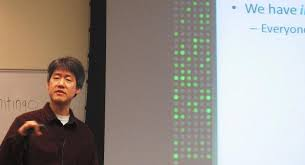
\includegraphics[width=.65\textwidth]{feedback-meetings-ms-research}
\caption{\emph{Crowd Feedback} \cite{Teevan:MobileFeedbackDuringPresentation} used during a presentation. The bar next to the slides shows one dot per participant in the meeting. The feedback dots fade out over time.}
\label{fig:related-work-crowd-feedback}
\end{figure}
% ADD MOBILE INTERFACE TOO AND MAKE PICTURE LOOK BETTARRR

\emph{Crowd Feedback} \cite{Teevan:MobileFeedbackDuringPresentation}, on the other side, is a system for displaying continuous, real-time feedback to the speaker in presentations. A responsive web application with a like and dislike button controls the feedback-system. The participants' reactions are shown with a red (dislike) or green (like) dot for each attendee in a sidebar next to the presentation slides (see figure \ref{fig:related-work-crowd-feedback}). An evaluation of the system showed that the participants felt more engaged with the presentation and connected to other listeners. Many users stated only having the possibility to like or dislike did not reflect enough options and that a button related to the speech pace might have helped. It was also noted that the sidebar was perceived as disturbing and made it harder to pay close attention to the presentation. This study and its conclusions have inspired the implementation of an instant feedback mechanism for listeners in the present work, however, instead of only having the binary like and dislike, the reactions are based on emojis, allowing for more insightful feedback.

The third study conducted by Microsoft Research concerns itself with the navigation through slides: \emph{Office Social} \cite{Chattopadhyay:OfficeSocialRemoteControl}, a PowerPoint plugin with companion smartphone app, allows presenters and listeners to navigate through PowerPoint slides using their mobile phones. Members of the audience can either browse the slides privately, or take over the control of the presented slides, allowing them to effictively steer the presentation or discussion. As in the present approach, Chattopadhyay et al.'s software allows members of the audience to review the slides privately, making it possible for latecomers to catch up and to generally estimate the length and direction of the talk. However, as their interface focuses on the navigation between slides, the preview of the slides is fairly small. Our approach tries to focus on the content of the slide and instead of offering big buttons to navigate around, makes use of intuitive swipe gestures. Another disadvantage is the overhead of having to download a smartphone application before the start of a presentation, as well as the limitation of the application only being available for Windows Phones.

\begin{figure}
\centering
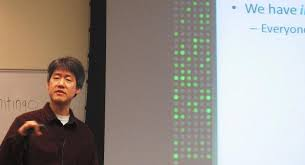
\includegraphics[width=.65\textwidth]{feedback-meetings-ms-research}
\caption{\emph{Office Social} \cite{Chattopadhyay:OfficeSocialRemoteControl}'s smartphone app interface. A preview of the slide is shown on top, followed by big buttons for navigating between slides.}
\label{fig:related-work-crowd-feedback}
\end{figure}

\section{General presentations}
Since lectures and meetings both are very specific forms of presentations, a few paragraphs should also be dedicated to general approaches in this third subsection.
One publication, which concentrates on polling and their real-time evaluation and rendering is \cite{Inoue:RealTimeQuestionnaire}: Inoue et al. present a system which distributes \emph{Microsoft PowerPoint} presentations using modern web-technologies while making it possible to alter and update the slides in presentation mode. This way questionnaires can be answered and their results displayed in real-time. Additionally, members of the audience can add annotations (both handwritten and digital) to slides. Although this approach seems very promising, pictures, videos and other types of media are ignored entirely. Moreover the interface seems too complicated to be displayed on small devices and is therefore only usable on laptops and maybe tablets.

Two more products, though not subject to scientfic research and more commercial than the approaches presented so far, are \emph{Mentimeter}\footnote{\url{http://www.mentimeter.com/}} and \emph{sli.do}\footnote{\url{http://sli.do}}. Both tools are web applications with real-time polling support, usable in any presentation. Both systems work very similarly: listeners go to the respective website and enter a presentation code to then be connected to the live voting. A handy feature Mentimeter offers is to query the device's location to determine the right presentation. Sli.do on the other hand also supports questions from the audience, which can be up-voted by the listeners, making it easy for speakers and participants in podium-discussions to answer the most relevant questions. Moreover, additionally to multiple-choice polls, sli.do also supports open questions and ratings. While the creators of Mentimeter provide a PowerPoint plugin, sli.do is not directly linked to any presentations. However, the popular canvas-based presentation-tool prezi\footnote{\url{http://prezi.com}}, offers seamless integration with the application. It is worth noting that prezi itself already offers mobile features out of the box: Presentations can be controlled remotely from the speaker's phone or tablet as well as be viewed and followed by members of the audience in real time, using a mobile application.

More web-based presentation tools include \emph{Google Slides}\footnote{\url{http://www.google.com/slides/about/}} and \emph{PowerPoint Online}\footnote{\url{http://office.live.com/start/PowerPoint.aspx}}. While PowerPoint Online seems to only offer a simplyfied version of the desktop application online, Google Slides also provides mobile features such as editing and authoring slides on phones or tablets and controlling them remotely.

To conclude this chapter, a few words should also be said about the JavaScript presentation library \emph{reveal.js}\footnote{\url{http://lab.hakim.se/reveal-js/}} and its accompanying visual edior \emph{slides}\footnote{\url{http://slides.com/}}. Reveal.js offers features such as remote controlling slides for the speaker and following presentations on personal devices for members of the audience. However, the installation to achieve the latter so-called \emph{multiplexing} functionality, is fairly complex and involves setting up a socket-io server, running the master-presentation statically and locally and uploading a client version of the presentation to a publicly accessible server. Reveal.js offers a decent online presentation library and could have served as a starting-point for the project presented in this thesis. However, due to their closed environment, tightly coupled code and lacking support for extensibility, we decided to instead implement an own presentation library (see chapter \ref{cha:implementation}, section \ref{sec:implementation-technologies-unveil}).
\chapter{Interactive Mechanisms}
\label{cha:mechanisms}

In a first step of identifying possible mechanisms which could make presentations more engaging and interactive, we analysed different types of presentations. There are several factors which determine these types, such as the size of the audience, the environment around and purpose of the presentation as well as the speaker and audience. In the following these factors will be described shortly to then present and discuss mechanisms these could profit from most.

\section{Factors}

\subsection{Audience Size}
One aspect which plays an important role in the type of presentation and thereby the interactive mechanisms applicable is the size of the audience. Different challenges present themselves, depending on the amount of listeners: While there might be a debate between speaker and audience in small group sizes, it is hard for audience members to directly communicate with a speaker during conferences or in large lecture halls. Shy or introvert attendees might remain unheard \cite{Bry:Backstage} and only a usually randomly chosen subset of people get the opportunity to ask audience questions after talks in conferences. At the same time estimating the audience's knowledge and interest as well as the general mood gets increasingly difficult both for the presenter and attendee as the number of participants rises. Additionally to the interaction between speaker and audience, another important factor is listener-listener interaction \cite{Moore:ThreeTypesOfInteraction}. Group-dynamics largly depend on the audience size and smaller groups usually perform better than big ones \cite{Phillips:GroupProblemSolving}.
The general conclusion therefore is that big audiences struggle to connect and interact with the speaker and each other and interactive tools must aim to strengthen the bidirectional bond between presenter and listeners. In smaller groups, on the other hand, the focus should be put on supporting the already existing dialogue and exchange between all participants of the presentation. As peer-pressure might rise in smaller groups and the better listeners know each other, ways of anonymously contributing to the outcome or flow of a presentation become more important.

\subsection{Presentation Environment}
% Remote vs co-located!
% setting: classroom vs. meeting vs. conference etc.
The environment of a presentation is described by all factors surrounding the presentation. One of them is the setting a talk is given in, in other words, if it is embedded in a meeting, a talk at a conference or a lecture at school or university. Other aspects worth considering are whether the audience is co-located or distributed and which technologies are available. As this work concerns itself only with mobile devices in the context of co-located presentations, difficulties added through remote presentations as well as missing technical equipment will be disregarded in this section. Instead, a closer look will be taken at the setting: In a lecture, it is desirable to measure the students' participation and engagement, as well as their understanding of a topic. In meetings, on the other hand, interactive mechanisms are more likely to aim for the promotion of collaboration between all participants. Conferences might search to foster the interactivity between attendees, to support networking. Instead of taking all possible scenarios into consideration, this work concentrates on business-related settings and explores mechanisms which foster collaboration.

Another part is the purpose of a presentation: McClain \cite{McClain:TypeOfPresentations} identifies four major types: informational, motivational, pursuasive and sales. According to him, informational presentations search to educate the listeners, while motivational speeches try to inspire the audience to take action. Pursuasive talks usually present new ideas or directions and have the goal of making the listeners re-think old approaches and consider or even embrace new ones. Sales presentations, lastly, often use elements of the other three categories with the aim of ``obtaining a decision at the presentation's end'' \cite{McClain:TypeOfPresentations}. While motivational, pursuasive and to some extend sales presentations often operate on an emotional level in the present moment, informational talks often include a way for listeners to re-visit the taught material through transcripts, lecture notes or handouts. Moreover, motivational, pursuasive and sales presentations focus on the goal of getting the audience to take action and therefore put more emphasise on the listeners than content-centric informational speeches. This creates two very distinctive needs for interactive mechanisms: on one side the ability for the audience to actively shape the path of the presentation, on the other hand the possibility to re-visit presentation slides (potentially including notes and additional material), after the end of a talk.

% welches material wird mitgenommen? wie können lectures erinnert werden? welches material nehmen wir mit? --> nachbereitung/handouts!
% motivational und pursuasive: mehr im hier und jetzt, memorable auf gefühlsebene!
% in manchen ist es einfacher das Publikum leiten zu lassen als in anderen (motivational & pursuasive)

\subsection{Speaker and Audience}
% tech savvyness for audience
% spontanität and flexibility for speaker --> when do I take questions? überfordert? etc.
% level of formality!
The last factor taken into consideration in this chapter are the speaker and listeners themselves. Depending on the individual interest, but also character traits such as introversion, listeners will be more or less likely to engage in a presentation actively \cite{Bry:Backstage}. The inter-attendee relationship as well as the relationship between attendees and speaker also plays a role in which mechanisms are appreciated and which are not \cite{Moore:ThreeTypesOfInteraction}: while it is common for listeners to jump into the role of the presenter in meetings with flat-hierarchies, the same behaviour is a rare sight in lectures or might even be deemed inappropriate or rude in more formal settings. When taking the speaker into consideration, the set of tools needed are more sophisticated than the ones necessary to only follow a presentation: Foremostly, speakers need a way of navigating through slide decks. It is desirable to have an overview of the entire presentation and while listeners only concentrate on the current slide, many speakers rely on notes or use timers, which also need to be placed in the interface.
Moreover, the presenter's personal traits, experience and bluntly talent, play a central role in the successful deployment of interactive mechanisms: the flexibility, confidence and technological expertise of a presenter all determine how distracting or even stressful certain features are perceived as and whether a speaker is able to react to these spontaniously \cite{Wacker:PresenterExperience}. It is therefore crucial to give speakers the ability to turn said mechanisms on and off. An important challenge which also arises with this question is how to design these mechanisms in a way that is neither perceived as intrusive nor interrupting (this will be discussed in more detail in chapter \ref{cha:design}).
To summarise, when developing interaction tools, it is vital to take a participant's personality and their relationship to other ones into consideration. In the context of presentations, shy listeners should be given tools to make them heard; presenters need full control of the mechanisms provided.

\section{Resulting Mechanisms}
With these aspects and challenges in mind, a multitude of different mechanisms can be derived. Although many more are thinkable, this section concentrates on the ones implemented in course of the thesis project. However, we will try to point out other possible features and provide resources to projects focusing on these. One point to keep in mind is that not all of the presented mechanisms work equally well in every environment but instead have scenarios they are best suited for and others in which they are practically rendered redundant. The ideal settings and key advantages of each of these mechanisms are summarised in table \ref{tab:mechanisms}.

% Speaker: Remote control
% Speaker: See next slide right and down, notes on phone or tablet/laptop!
%
% Following slides on personal device
% Questions
% Anonymity
% Polls
% Reactions (Emojis) -- tell how these can engage the people more, not only about how they provide feedback to presenter!
% Annotating slides and sharing content (!) --> not really studied yet, so cool!

\subsection{Remote Control}
One mechanism of special importance for speakers is the ability to control slides and navigate through them. As many presentations involve more than just one speaker and can profit from sharing control over slides with others \cite{Chattopadhyay:OfficeSocialRemoteControl}, any amount of presenters should be able to be connected at any given point. Controlling should be possible from any personal device, may it be a laptop, tablet or mobile phone, giving the speakers maximal freedom.

While using arrow-keys in a desktop environment feels natural to navigate between slides, the native equivalent on touch-devices are swipe gestures. These are more accurately and faster when operating a phone with one hand \cite{Lai:SingleHandedThumbInteraction} and are less prone to error when used eye-free \cite{Negulescu:TapSwipeMove} and should therefore be prefered over buttons, clustering the interface.

\subsection{Following Slides}
% also gives latecomers the chance...
For members of the audience, one important feature, both in the context of re-visiting slides, to accommodate individual learning paces \cite{Cheng:TreebasedOnlinePresentations} and even to give latecomers a chance to catch up with the presentation \cite{Chattopadhyay:OfficeSocialRemoteControl}, is to be able to independently follow the slides. This should again be possible on any personal device and focus on the slide content, in a way that maintains the readibility of all text. The mechanism can be designed in many different ways and could even allow listeners to remote control the presentation \cite{Chattopadhyay:OfficeSocialRemoteControl}, our implementation however only provides individual slide navigation on the personal device. Additionally, the progress of the presentation should always be synchronised with the individual devices, allowing listeners to truely follow along. This basic mechanism can be extended to offer features such as turning the synchronisation on and off (effectively allowing to navigate freely and jump back to the presenter's state) or to only allow listeners to see the last slide the presenter has already shown.

\subsection{Paths}
Also connected to navigation and following slides is the possibility to offer different paths through the presentation. Especially in informational talks these can account for different backgrounds and levels of knowledge in the audience, they however, also make it possible to get listeners more involved in shaping the presentation. Paths should both be accessible to each audience member individually (for further reference or to catch up on a topic), as well as on the projector (e.g. by polling, as discussed in the next subsection).
The possibility to flexibly navigate through a presentation has proven to be one of the biggest advantages of canvas-based presentations \cite{Lichtschlag:CanvasPresentationsInTheWild} and have a wide field of application. The scenarios this thesis concentrates on are the following: On one hand, the paths can cover different levels of details (e.g. \emph{overview}, \emph{regular} and \emph{detailed}), as well as providing a way of skipping certain slides without having to navigate through all of them (e.g. skipping the introduction). Another option would be to let the audience decide between entirely different topics, depending on their personal interest. While canvas-based presentation tools like Prezi innately offer this flexibilty, slide-based tools often only make this behaviour possible by manually skipping over slides, which can interrupt the flow of the presentation \cite{Dieberger:NarrativeFlow}. PowerPoint extensions enabeling advanced forms of navigation, as well as the presenter looking through slides before projecting them are discussed in \cite{Dieberger:NarrativeFlow}, \cite{Nelson:PalettePaperInterface} and \cite{Signer:PaperPoint}, the latter, however, will not be part of our implementation.

\subsection{Audience Questions}
Another feature, well-suited for informative talks, is the possibility for members of the audience to ask questions. Another scenarios are big crowds, in which it is hard to be heard as an individual. A tool specifically designed for such settings is sli.do, which was already introduced in chapter \ref{cha:related-work} section \ref{sec:related-work-general}.
More generally, such mechanism should enable members of the audience to submit questions for the presenter to answer. These questions should either be displayed directly, or collected for the presenter to go through at the end of the presentation, depending on their preference and flexibility. This mechanism also highly depends on the presentation environment: In a classroom, questions should be answered immediately, while conferences usually only allow them at the end of talks. Questions could moreover only be visible to the presenter, or every participant. Concentrating on business-related settings, we propose a question feature which allows audience members to submit questions at any point of the presentation. These should be accessible for every attendee, to spark others' interest and participation. From the presenter's point of view, questions should be displayable instantly, at the end of the talk or any time inbetween, leaving the decision when to react to questions to each individual speaker.

% what does it mean for the presenter - take questions right away or in the end?

\subsection{Polls}
Another possibility to ask questions is polling. Although polls might also be generated by listeners, we propose a mechanism which lets the speaker create them. To give presenters more flexibility and because questions often only arise during talks \cite{Esponda:ElectronicVotingOnTheFly}, these surveys should be creatable in the preparation for a speech as well as on-the-fly, during presentations. This mechanism can help getting to know ones listeners (relationship between listeners and speaker), as well as estimate a crowd's mood (big audiences) and is especially useful in combination with paths. If supporting anonymous voting, relying on electronical aids instead of raising hands can also be benificial in smaller groups \cite{Esponda:ElectronicVotingOnTheFly}.
While a big number of different polling mechanisms are conceivable (open questions, ratings, multiple choice, as well as different ways of visualising the results), single choice voting and visualisation in a bar-chart serve as a starting point for our approach. Another detail lies in when the results are presented: they can either be rendered as soon as a user chooses his or her answer or only after everybody has given their votes.
To summarise, the identified requirements for such mechanism are creation beforehands and during the presentation, real-time polling and data-visualisation as well as anonymity of the voting process.

\subsection{Reactions}
As described before, especially bigger crowds suffer from a lack of interaction possibilities between speaker and audience but also between members of the audience. While the latter is discussed in \cite{Bry:Backstage}, the present work focuses on the interaction between speaker and listeners. Besides the difficulity of asking questions, which was already covered, the main problem for the presenter is to estimate the crowd's mood, which is why we suggest a mechanism that lets attendees send real-time feedback to the speaker. This functionality is based on \cite{Teevan:MobileFeedbackDuringPresentation}; as highlighted by Teevan et al., however, their simplistic approach of just offering \emph{likes} and \emph{dislikes} is not faceted enough to represet the full range of emotions listeners can feel during a presentation. It is therefore important to provide more detailed feedback.
These reactions can either be displayed only to the speaker, or to the entire audience. The latter might distract listeners \cite{Teevan:MobileFeedbackDuringPresentation}, however, also holds the potential to encourage others to also react to the current slide and strenghten listener-listener bonding. While this mechanism is expected to work well in bigger crowds, it will likely introduce an unnecessary technical burden to smaller groups, in which it is easier to estimate the attendees' mood. 

\subsection{Content Sharing}
In contrast to live reactions and questions, content sharing is especially suited for smaller audiences. As discussed before, tools for smaller groups should strengthen the already possible dialogue between all participants. These scenarios make it possible for listeners to actively get involved in the presentation and not only shape the path through, but also the content of such. While adding subslides to a slide deck after a presentation \cite{Cheng:TreebasedOnlinePresentations} and text-based annotations \cite{Inoue:RealTimeQuestionnaire, Myers:CollaborationPDAs} during talks have already been discussed in previous work, to our knowledge, no other study has concerned itself with the possibility of adding listener-generated slides and multi-media content in live presentations. While being an exciting opportunity to explore a widely untouched research subject, this mechanism empowers listeners and transforms presentations entirely by combining classic slides with brainstroming-like interactions and related multi-media content. While the potential of this mechanism will be further discussed in chapter \ref{cha:conclusion}, the requirements for this functionality should shortly be defined: It should be possible for any listener to add their own content to any slide. This content includes text, websites (per link), videos and uploaded images (e.g. taken with their personal devices). Presenters should have a way of deciding whether to accept the contribution and if it should be added as a subslide or main slide. Moreover, this mechanism requires a lot of flexibility from the speaker, which is why it is important to allow them to turn off or silence the functionality, providing sensible fallbacks. While content sharing can transform a presentation into an interactive and collaborative effort in smaller groups, the functionality will likely lead to chaos in big groups, without further interface changes.

Now that the implemented mechanisms are clarified and their requirements defined, the next chapter deals with the design and user experience of the application.

\begin{table}
\caption{Overview of resulting mechanisms, with their key advantages and optimal usage scenarios.}
\label{tab:mechanisms}
\centering
\def\rr{\rightskip=0pt plus1em \spaceskip=.3333em \xspaceskip=.5em\relax}
\setlength{\tabcolsep}{1ex}
\def\arraystretch{1.20}
\setlength{\tabcolsep}{1ex}
\small
\begin{english}
\begin{tabular}{|p{0.2\textwidth}|p{0.35\textwidth}|p{0.35\textwidth}|}
\hline
   \multicolumn{1}{|c}{\emph{Mechanism}} &
   \multicolumn{1}{|c}{\emph{Improvements}} &
   \multicolumn{1}{|c|}{\emph{Ideal Scenario}} \\
\hline\hline
   {\rr Remote Control} &
   {\rr More flexibility for presenter(s)} &
   {\rr Any, especially mutli-speaker presentations}
   \\
\hline
   {\rr Following Slides} &
   {\rr Accounts for individual pace; can replace hand-outs} &
   {\rr Any, especially informational presentations for later revision}
  \\
\hline
   {\rr Paths} &
   {\rr Interactivity and possibility to shape presentation for audience} &
   {\rr Any, especially informational}
   \\
\hline
   {\rr Audience Questions} &
   {\rr Anonymity; possibility to be heard in big crowds } &
   {\rr Big audiences; small groups for anonymity}
  \\
\hline
   {\rr Polls} &
   {\rr Bond between speaker and audience by querying listeners' interest, mood and knowledge} &
   {\rr Usage with paths; big audiences; small groups for anonymity}
   \\
\hline
   {\rr Reactions} &
   {\rr Speaker-audience and listener-listener interaction} &
   {\rr Big audiences}
   \\
\hline
   {\rr Content Sharing} &
   {\rr Possibility to shape presentation for audience; slide-content by adding related resources} &
   {\rr Small groups}
   \\
\hline
\end{tabular}
\end{english}
\end{table}
\chapter{Application Design}
\label{cha:design}

After defining the mechanisms which will be implemented, in a next step, the general application flow will be described, as well as offering insight into the user experience design of the parts of the application.

\section{Application Flow}
The flow and usage of the application is separated into two parts: the creation and authoring of the presentation and giving the presentation. Because the technical details of how slide decks are composed are covered in chapter \ref{cha:implementation}, this chapter focuses on the user interface and interaction design of the software from the speaker's and the audience's point of view, during the presentation.

The slides are generally served either from a publicly accessible server or, if all participants are in the same network, locally from the presenter's computer. This means, at the beginning of the presentation, all attendees have to navigate their personal devices' browsers to the set up address (usually a combination of IP address and port). To make this step easier, QR codes pointing to the address can be shown on the first slide or e-mails can be sent out to all participants before the start of the presentation.

The software supports three different modes out of the box: default (i.e. listener), presenter and projector mode. Depending on the mode, a certain set of features are activated, allowing the presenter to have a different interface and more controls than the listeners and to only show the current slide in projector mode. Modes are activated via query-strings in the url: The speaker navigates the browser of the device connected to the projector to the url of the presentation and adds the query parameter \printtt{mode=projector}. On his or her personal device, the mode is set to \printtt{presenter}. If no query parameter is given, the application defaults to the listener mode.

% Base CSS: responsive, if content is too big, everything is uniformly scaled.


% Application Flow, Modes, How does the application work in general?
% Design aspects, sketches, wireframes, thoughts and überlegungen behind design details

% As described before, it is important for the presenter to be in full control of all mechanisms --> make it easy to add or remove them and to configure!

% Wacker: research has shown that technological problems are the main reason for negative presentation experiences for the speaker. ``Therefore, presentation software should take special care to avoid technological problems and assist the presenter if they should occur''

% We believe it is still important for the speaker to have an overview of the current slide as well as upcoming ones and be able to see notes on the presenter interface

% General requirements: be viewable on every device, work in real-time!

% Emojis
% Find more studies about this! think: facebook, the conference Paulo went to etc. (maybe add photo of audience showing emoji faces!)
% It is therefore important to provide more detailed feedback. Following the evaluation in \cite{Teevan:MobileFeedbackDuringPresentation}, the mechanism proposed in this thesis offers three emotions (approval, laughter, boredom) and three request types (louder, speed up, slow down).

% Polls: Describe why freeze navigation while voting and only allow voting when started by presenter
\chapter{Implementation}
\label{cha:implementation}
% short overview; why web -- use references!
% speak about quick prototyping possibilities and how it's easier to roll out updates and how nobody needs to download an app on their phone to interact with the presentation
% say something about open source and why all the code is online on github!

This chapter dives into the technical implementation details of the thesis project and gives an overview of the used technologies and explains why these were chosen over others. Like many other projects in this area \cite{Bry:Backstage, Cheng:TreebasedOnlinePresentations, Esponda:ElectronicVotingOnTheFly, Inoue:RealTimeQuestionnaire, Teevan:MobileFeedbackDuringPresentation, Triglianos:InteractiveWebPresentationsImpress}, the project is realised as a web application. This has many advantages, from modern web technologies' quick prototyping capabilities to the web's general cross-platform and cross-device nature, the project has profitted from the dynamicity of the internet and the rapid evolvement of JavaScript over the past years.
Although native sharing features of smartphones cannot be used due to the choice of platform, the advantages that come with this decision outweigh the disadvantages, as I like to think for both users and developers: as nobody has to download any apps to their devices, it is easier to bring the audience to use the developed application \cite{Triglianos:InteractiveWebPresentationsImpress}. The major advantages for developers on one hand is the ability to only concentrate on one platform, instead of developing different applications for different operating systems (mobile and desktop), on the other hand the web is built for rapid prototyping as it is extremely easy and fast to roll out new updates, without distributing them through the App Store or Play Store and without the need for users to manually update their apps. The chosen JavaScript library React, however, offers the possibility to cross-compile applications to different devices using React Native, which should make it fairly easy to port the existing web application in the future.

As it was important to achieve fast response times and because \emph{WebSockets} have successfully been deployed in the real-time features of other presentation tools \cite{Inoue:RealTimeQuestionnaire, Triglianos:InteractiveWebPresentationsImpress}, this technology has also been used in this thesis project, to handle the communication between clients and server.

A few words should also be said about the distribution of this project. Without the vibrant open-source community, many of the frameworks and libraries used in this project would not exist. For this reason and to give back to this community, all the libraries developed during this project are published as open-source on my GitHub profile\footnote{\href{https://github.com/irisSchaffer?tab=repositories}{\textsf{https://github.com/irisSchaffer/}}} and freely available for anyone to use.

\section{Project Scope}
\label{sec:implementation-scope}
% What's the general scope of the project? Why is everything on the client and 
% not the server? etc.
Before jumping into technical details, the scope of the project should be discussed. As the aim of the present work is to explore ways of incorporating mobile devices into presentation workflows, the goal of the project was to use an easily extensible presentation library to then build the mechanisms discussed in the previous chapter.
As the focus was placed on the interaction possibilities between speaker and audience, the creation of the presentation for the speaker or the management of slides and presentations were out of scope. Therefore the server used for connecting different users to the presentation was kept as simple as possible, allowing any potential other developer to work with their own servers and technology stacks.

In total, a system with several ways of interacting with the presentation from mobile or desktop devices was created, putting emphasise on mobile-optimised views and navigation possibilities. This system includes synchronisation of navigation state and state changes between viewers and speaker, the possibility to add sub-slides during the presentation for the audience, a speaker-view showing the next slides and controls, real-time voting (both created on-the-fly and prepared beforehands) and the possibility to create different paths through the presentation. In the following the technologies used in the project will be analysed and described to then discuss implementation details, problems and solutions of the mentioned components.

\section{Technologies}
\label{sec:implementation-technologies}
% Which technologies were chosen and why?
% How do they generally work? To a level on which the reader can
% understand the rest of the implementation details
% A few words about responsive design and media queries would probs be good
% a few words about babel and es6

The project generally tries to follow best-practices in web development and utilises modern CSS3 and JavaScript features and frameworks. The software is written in ECMA\-Script\-2015, makes use of the \emph{node package manager}\footnote{\url{https://www.npmjs.com/}}(short \emph{npm}) for managing dependencies and \emph{Babel} to transpile to ECMA\-Script\-5. Additonally to relying on CSS3 features, this project also uses \emph{Sass}\footnote{\url{http://sass-lang.com/}} as a CSS pre-processor. Media-queries allow for mobile-friendly views.

On the front end, which this project focuses on, the JavaScript library \emph{React} is the framework of choice, additionally applying the \emph{reactive programming} paradigm using \emph{RxJS} to allow for a simpler interface for event-driven operations. The communication between client and server is handled by \emph{socket.io}\footnote{\url{http://socket.io/}}.
This section tries to introduce the reader to the main technologies used to establish a base on which the following technical implementation details can be understood.

\subsection[ECMAScript2015 and Babel]%
             {ECMAScript2015 and Babel%
             \protect\footnote{\url{https://babeljs.io/}}}%
\label{sec:implementation-technologies-es6}
% it's a recommendation, but it takes long until browsers implement it and users update their browsers.
JavaScript undoubtly is an integral part of front end web development and since the emergence of server-side JavaScript with Node.js\footnote{\url{https://nodejs.org/en/}} and its package manager npm has developed into a programming language widely used by web developers \cite{gpm-meta-transcompiler}. Both PYPL\footnote{\url{http://pypl.github.io/PYPL.html}} and TIOBE\footnote{\url{http://www.tiobe.com/tiobe_index}} programming language indices rank JavaScript among the top 10 programming languages (PYPL at 5, TIOBE at 7 at the time of writing) \cite{gpm-meta-transcompiler}. Stack Overflow's 2015 Developer Survey even places JavaScript as the number 1, most-used programming language with 54.4\% and JavaScript, Node.js and AngularJS\footnote{\url{https://angularjs.org/}} all three rank amongst the top 5 languages developers expressed an interest in developing with \cite{stackoverflow-developer-survey}.

However, like any front end technology, JavaScript suffers from slow end user adoption, as a multitude of browser versions exist for different devices and operating systems and many people still do not auto-update their browsers. Another factor is the time it takes for browser-vendors to implement new ECMAScript standards (the standard behind JavaScript) and roll out said updates. This is exactly what is happening with the new ECMAScript standard, ECMA-262, commonly known as ECMAScript 2015 or ES6: Although the General Assembly has adopted the new standard in June 2015 \cite{ecma2015}, \emph{Kangax' ECMAScript compatibility tables}\footnote{\url{https://kangax.github.io/compat-table/es6/}} still show a fairly low level of adoption, especially among mobile browsers. ES6 makes JavaScript easier and more efficient to write by providing new semantics for default values, arrow-functions, template-literals, the spread operator or object destructuring \cite{es6}. It also makes JavaScript easier to understand and safer to develop, with the introduction of block-scoped variables (\texttt{let} and \texttt{const}) and finally offers native support of modules and promises \cite{es6}.
As these features are all included in the new ECMAScript standard, it is safe to assume browser-vendors will implement them in the near future. Until then, developers who want to already make use of them, can \emph{transpile} ECMAScript 2015 code into ECMAScript 5, which is exactly what Babel does. With over $650000$ downloads in March 2015 (according to npm) and companies like Facebook, Netflix, Mozilla, Yahoo or PayPal using this transpiler \cite{babel-users}, Babel is the de facto standard solution to transpile to ECMAScript 5 and was also chosen for this project.

\subsection{Reactive Programming}
\label{sec:implementation-technologies-rxjs}

Another problem with JavaScript, although integral part of the reason for its high popularity, is its asynchronous nature. Especially when working with highly interactive parts, the prime example being user interfaces, sequential programming quickly gets too inflexible to handle complex, event-driven applications \cite{reactive-programming-survey}. But also on the server, the possibility to concurrently serve a multitude of different clients, is crucial. In these cases JavaScript offers \emph{event listeners} -- functions called once a certain event happens. However, these event listeners or \emph{asynchronous callback} \cite{reactive-programming-survey}, oftentimes executes more asynchronous code and in turn has to wait for another event, and another one, and another one... which can result in something known and dreaded by most any JavaScript developer: \emph{Callback Hell} (see programm \ref{prog:implementation-technologies-rxjs-callback-hell}).

\begin{program}
\caption{\emph{Callback Hell} -- Nested callbacks in JavaScript. Simplified method taken from a previous project, which authenticates a user, creates a new google calendar for them and then saves the user to one\'s own database, to then redirect them. \texttt{\{...\}} is used to shorten the code, error-handling was also omitted in the example for simplicity.}
\label{prog:implementation-technologies-rxjs-callback-hell}
\begin{JsCode}
router.get('/callback', function(req, res, next) {
  var code = req.query.code;
  var name = JSON.parse(req.query.state);

  // get token from oauth library
  oauth2Client.getToken(code, function (err, tokens) {
    // load configuration
    Configuration.findOne({}, function (err, configuration) {
      var calendar = google.calendar('v3');
      // save to google calendar
      calendar.calendars.insert({...}, function (err, cal) {
        var member = new Member({...});
        // save member to own database
        member.save(function(err, member) {
          return res.redirect(getRedirectionUrl(name) + '&success=true')
        });
      });
    });
  });
});
\end{JsCode}
\end{program}

Different approaches have been employed to lower the hurdle of writing asynchronous code, one of them being \emph{promises}: A promise is a value, yet to be computed \cite{reactive-vs-promises}. A promise can be a) pending (if it has not been assigned a value yet), b) resolved (if it has been assigned a value) or c) rejected (if an error occurred). In ECMAScript 2015 promises these objects can then be queued using the \texttt{then} keyword, to execute asynchronous code in a certain sequence (see programm \ref{prog:implementation-technologies-rxjs-promises}).

\begin{program}
\caption{\emph{Promises} -- Simple example of chaining ECMAScript 2015 promises with \texttt{then} and \texttt{catch}.}
\label{prog:implementation-technologies-rxjs-promises}
\begin{JsCode}
var promise = new Promise(function(resolve, reject) {
  asyncCall(function(error, data) {
    if (error) {
      reject(error); // reject the pending promise
    } else {
      resolve(data); // resolve the pending promise
    }
  })
})

promise
  .then(function(data) {
    // this is executed after asyncCall returns
    // other asyncronous calls can be placed here
  })
  .catch(function(error) {
    // this is executed if an error occurs somwehere along the way
  })
\end{JsCode}
\end{program}

However, promises can still create nested callbacks, especially when chaining promises that rely on other promises' resolution \cite{reactive-vs-promises}. This is where \emph{reactive programming} comes in: The reactive programming paradigm works with streams of events, in which every event is handled as a new value and all other parts depending on this value are re-computed upon arrival of such a new value. To demonstrate this I would like to use Bainomugisha et al.'s illustrative example of a simple addition \cite{reactive-programming-survey}:

\begin{JsCode}
var v1 = 1
var v2 = 2
var v3 = var1 + var 2
\end{JsCode}
%
In sequentially executed code, \texttt{v3} will hold the value $3$, no matter if or how \texttt{v1} or \texttt{v2} change. In reactive programming, however, \texttt{v3} will be re-computed as soon as either one of the values it depends on change \cite{reactive-programming-survey}. This way for a drag-and-drop feature, for example, the move of the mouse, continuously sending its location, could directly alter the position of an element in a page. JavaScript does not directly support reactive programming, but other, more functional languages, which can be transpiled to JavaScript, do. Another way of adding reactive programming concepts to JavaScript is using a library, such as \emph{Bacon.js}\footnote{\url{https://baconjs.github.io/}} or the one chosen for this project, \emph{ReactiveX}\footnote{\url{http://reactivex.io/}}. ReactiveX provides libraries for a multitude of different programming languages, C#, C++, Java and of course JavaScript among them. The latter, called \emph{The Reactive Extensions for JavaScript} or short \emph{RxJs}, allows for the simple creation of event streams (\emph{Observables}) from browser events or promises directly and uses the same method names JavaScript developers are familiar with from array-methods, most notably and well-known \texttt{map}, to apply a method to every element in the incoming stream and \texttt{filter}, to only let a subset of events pass. These methods can be chained to sequentially alter a value (see programm \ref{prog:implementation-technologies-rxjs}).

\begin{program}
\caption{\emph{RxJS} -- simplified example of the touch controls used to swipe to the next or previous slide. An Observable is created from the browser's \texttt{touchmove} event and is then transformed with \texttt{map} and \texttt{filter}, to in the end call the \texttt{navigate()} method with the direction the user swiped into.}
\label{prog:implementation-technologies-rxjs}
\begin{JsCode}
this.moveObservable = Observable.fromEvent(document, 'touchmove')
  // data: event object with array of touches
  .filter(this.touchStarted) // only procede if touchstart is set to true
  .map(this.toXY) // transform initial event data to latest touch's xy position
  // data: \{x: xPosition, y: yPosition\}
  .map(this.toDirection) // transform xy position to direction literal
  // data: right/left/up/down
  .do(this.resetTouchStart) // set this.touchStarted to false
  // data: right/left/up/down
  .subscribe(this.navigate); // call this.navigate() with direction data
\end{JsCode}
\end{program}

Additionally to Observables, RxJs also knows \emph{Subjects}, which combine both a source of events and a consumer of such. Subjects are Observables, but also Observers at the same time and can be used to broadcast values to several consumers \cite{rxjs-docu}.

\subsection[React]%
             {React%
             \protect\footnote{\url{https://facebook.github.io/react/index.html}}}%
\label{sec:implementation-technologies-react}
% explain base concept of having re-usable components and how they are defined!
% get some HTML code in there :)

As this project concentrates on the front end, a mature JavaScript framework was searched for. After previous experience with the big and complex, but slow AngularJS, because of promising performance benchmarks \cite{react-benchmarks} and simply to explore new JavaScript libraries, I decided to give React a try. Since Facebook started developing React in 2013, it has challenged existing approaches and set new standards in front end web development \cite{introduction-to-react}. Instead of creating an entire MVC framework for the front end, React really concentrates on the view by offering a way of creating independent, lightweight view components. This gives React the huge advantage of beating other front end frameworks by far in performance benchmarks \cite{react-benchmarks}. Moreover, \emph{React Native}\footnote{\url{https://facebook.github.io/react-native/}} would make it possible to port the application to different mobile operation systems fairly easily.
The arguably most important method these re-usable, lightweight components implement is the \texttt{render} method, defining what HTML or JSX\footnote{\url{https://facebook.github.io/jsx/}} should be rendered by the browser:
\begin{JsCode}
export default class HelloWorld extends Component {
  render() {
    return (<h1>Hello World!</h1>);
  }
}
\end{JsCode}
%
The created Component can then be rendered into the virtual React DOM, JSX makes it possible to simply use the name of the component to create it:
%
\begin{JsCode}
ReactDOM.render(
  <HelloWorld />,
  document.getElementsByTagName('body')[0]
);
\end{JsCode}
%
This would simply put an \texttt{h1} element with the text \texttt{Hello World!} into the \texttt{body} element of the HTML page. Additionally to the \texttt{render} method, components also have a \emph{state} and \emph{properties}(\texttt{props}), through which they can communicate with other components and maintain their inner state. \texttt{props} are passed in to the component during creation, in JSX this can be achieved by simply passing them in as XML attributes:
%
\begin{JsCode}
  <HelloWorld greeting="Hi" />
\end{JsCode}
%
This could in turn be used in the \texttt{HelloWorld} component's \texttt{render} method:
%
\begin{JsCode}
  render() {
    return (<h1>{this.props.greeting} World!</h1>);
  }
\end{JsCode}
%
The children of a component are also available through \texttt[this.props.children]. The \texttt{state} variable, on the other hand, is responsible for handling internal updates e.g. through user interaction \cite{react-docu}. To alter the state, the method \texttt{setState} can be used, which will cause an update and re-rendering of the component. So if in the above example, the word ``World'' should be changed to something else by the user, a text field with an event handler can be added inside the component:
%
\begin{JsCode}
// set default state and props...

componentWillMount() {
  // create observable from change event on input
  this.observable = Observable.fromEvent('change', this.refs.input)
    .pluck('target', 'value') // extract input text
    .subscribe(this.update) // call update with value
}

componentWillUnmount() { this.observable.unsubscribe() }

update(text) { this.setState({name: text}) }

render = () => (
  <div>
    <h1>{this.props.greeting} {this.state.name}!</h1>
    <input value={this.state.name} ref="input" />
  </div>
)
\end{JsCode}
%
Now, whenever a user changes the text in the \texttt{input} field, the RxJS Observable will receive a new value (a change event). The \texttt{value} of the field is extracted on line $6$ and used to then update the state in the \texttt{update} method, which is implicitly called with the value passed through the Observable chain.

The two methods \texttt{com\-po\-nent\-Will\-Mount}, \texttt{com\-po\-nent\-Will\-Un\-mount} as well as \texttt{com\-po\-nent\-Did\-Mount}, \texttt{should\-Com\-po\-nent\-Up\-date}, \texttt{com\-po\-nent\-Will\-Up\-date}, \texttt{com\-po\-nent\-Did\-Up\-date} and \texttt{com\-po\-nent\-Will\-Re\-ceive\-Props} are \emph{lifecycle methods}, called whenever the component is created, updated or destroyed.

As an end note on React, and a transition to the core presentation library, I want to add that React components can be nested, which is at the core of the project developed for the present thesis. To make it as easy as possible for other developers to use the created libraries, a presentation is built just as a usual HTML page, using JSX to reference the custom React components (see program \ref{prog:implementation-technologies-react}).
%
\begin{program}
\caption{Nested React components. In this example, a 1-slide-long presentation is created.}
\label{prog:implementation-technologies-react}
\begin{JsCode}
<UnveilApp>
  <Slide name="start">
    <h1>Unveil</h1>
    <h2>a meta presentation</h2>
    <Notes>Greet people and welcome everyone</Notes>
  </Slide>
</UnveilApp>
\end{JsCode}
\end{program}

\subsection[unveil.js]%
             {unveil.js%
             \protect\footnote{\url{https://github.com/ostera/unveil.js}}}    
\label{sec:implementation-technologies-unveil}
% explain how this was developed together with Leandro, explain general parts like router, navigator, UnveilApp
% Give overview over controls in here.
% Also talk about the mobile style sheets / responsive design and the TouchControls, which I also implemented alone.
% (mention that this part is unit tested with jest(https://facebook.github.io/jest/))

As a presentation layer, this project uses the open-source JavaScript library \textit{unveil.js}, which was developed by Leandro Ostera and myself in the beginning of the project and which I extended and adapted to my needs in an own fork\footnote{\url{https://github.com/irisSchaffer/unveil.js}} during the project. This fork will be covered in section \ref{sec:implementation-unveil} of this chapter, until then, a short overview of the different parts of unveil.js is given and key concepts of the library are discussed. Screenshots of what unveil.js looks like can be found in figure \ref{fig:implementation-technologies-unveil-screenshots}.

%\begin{figure}
%\centering\small
%\begin{tabular}{cc}
%\FramePic{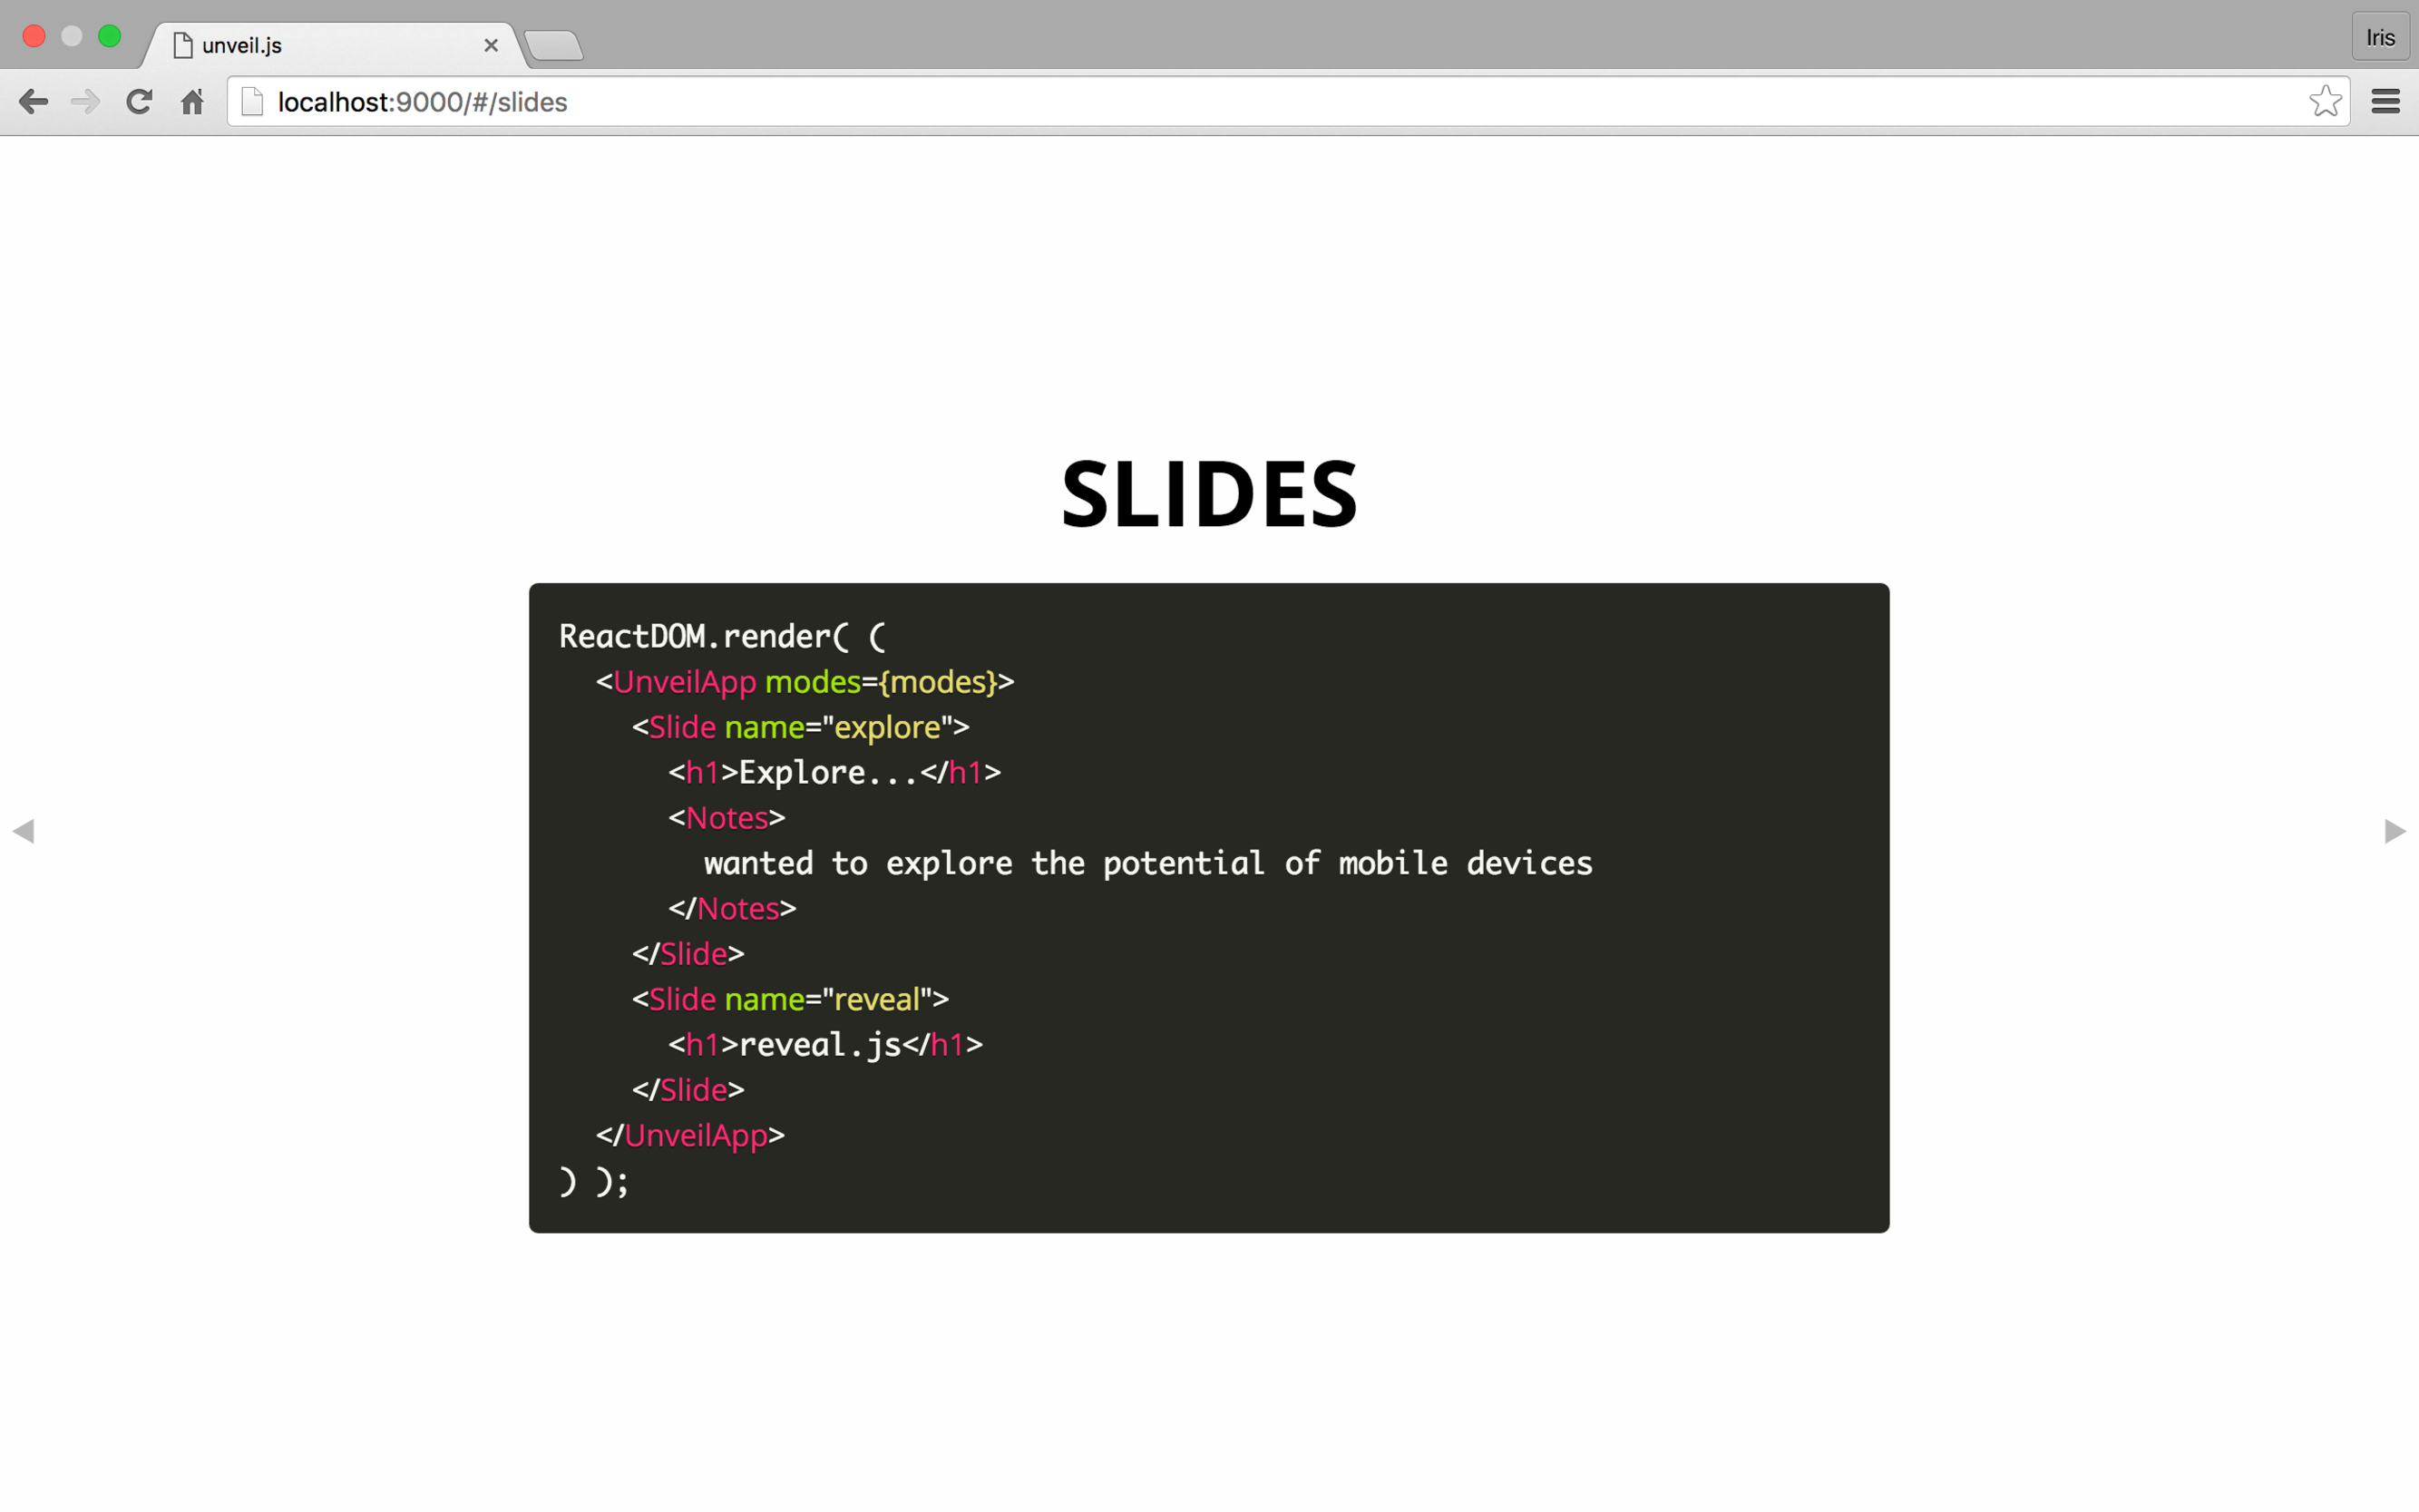
\includegraphics[width=0.5\textwidth]{unveil-screenshot}} &
%\FramePic{\includegraphics[width=0.3\textwidth]{unveil-screenshot-mobile}} \\
%(a) & (b) 
%\end{tabular}
%\caption{Screenshots from desktop (a) and mobile (b) view of unveil.js.}
%\label{fig:implementation-technologies-unveil-screenshots}
%\end{figure}

\begin{figure}
\centering
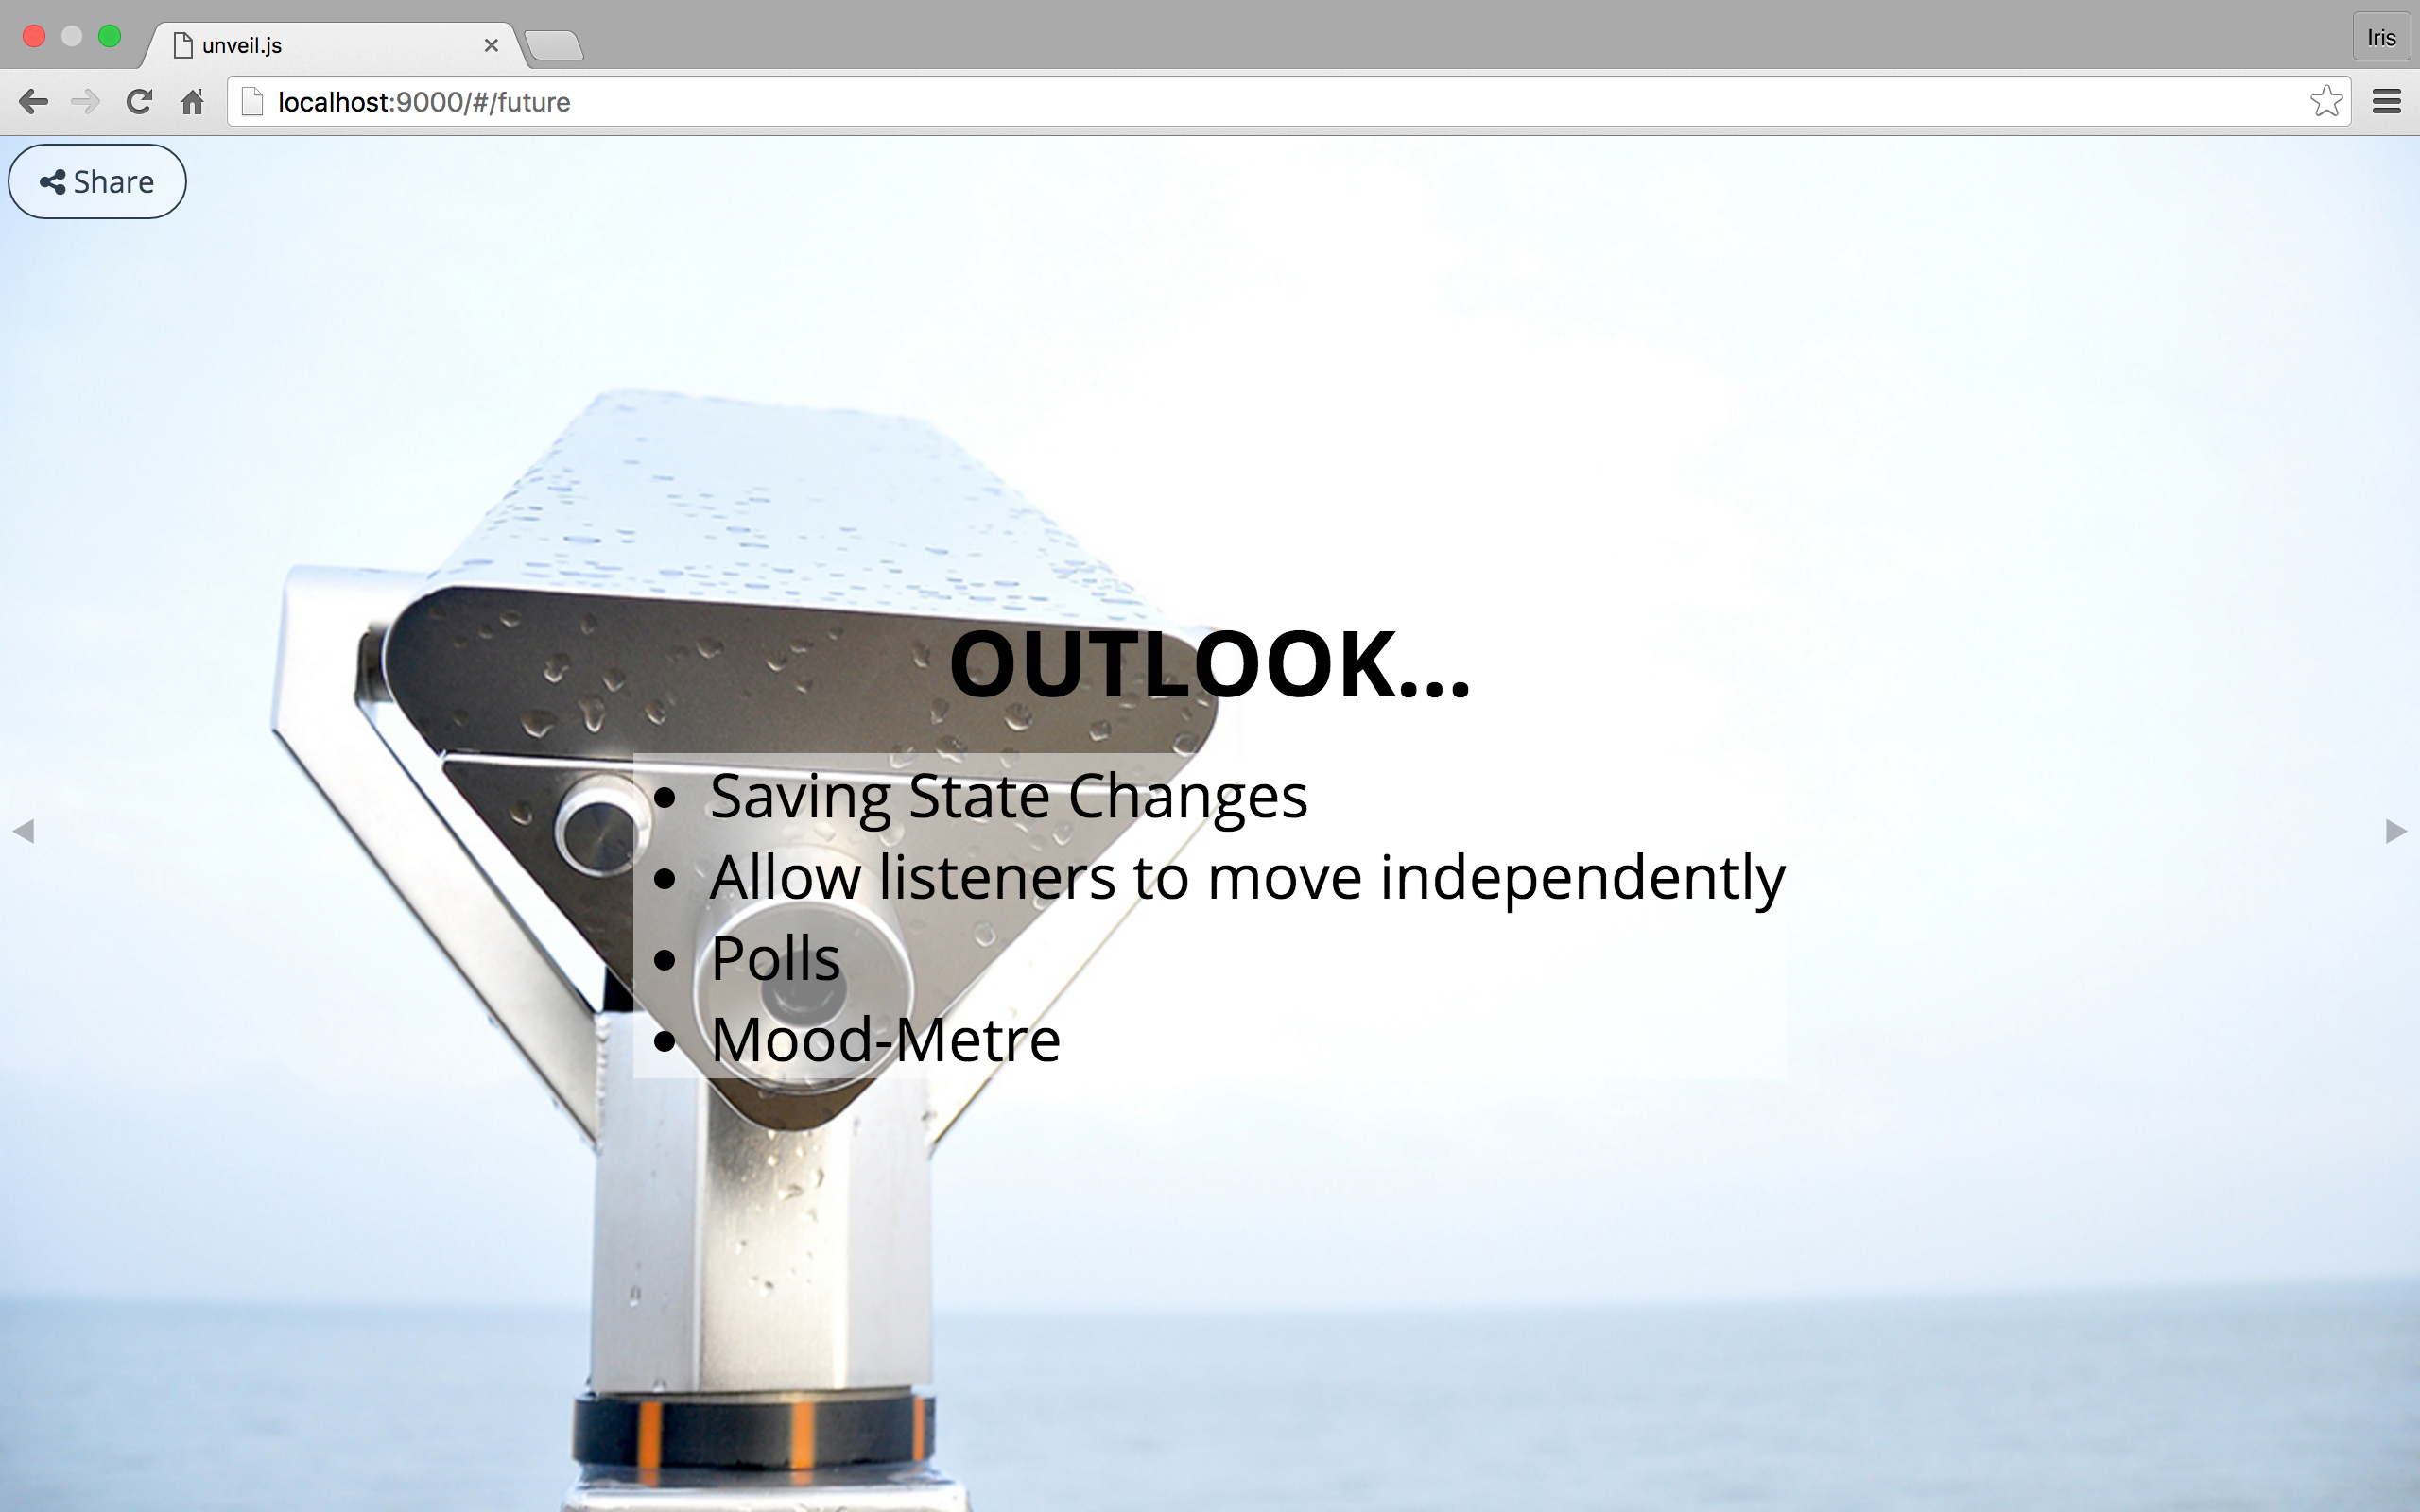
\includegraphics[width=0.65\textwidth]{presentation-screenshot}
\caption{Screenshot of an example slide with unveil.js, using interactive extensions discussed in section \ref{sec:implementation-interactive}.}
\label{fig:implementation-technologies-unveil-screenshots}
\end{figure}

Generally, unveil.js operates on a $2$-dimensional slide-space: Every slide can have a next and previous slide in $x$, as well as in $y$-direction. To generate the $y$ axis, slides can be nested in other slides. These slides have an optional unique name as well as an index in the slide-tree, which they are identified by. As shown in program \ref{prog:implementation-technologies-react}, slides are created inside the component \texttt{UnveilApp}, the core of unveil.js. This component configures and sets up the entire application based on optional configuration passed in as properties.
There are a few concepts unveil.js is built around to allow for extensibility and configurability, namely \emph{presenters}, \emph{controls} and \emph{modes}:
%
\begin{itemize}
\item \textbf{Presenters} define the way slides are rendered, e.g. show notes, upcoming slides or hide them.
\item \textbf{Controls} control a part of the application, e.g. navigating from one slide to the next using the arrow keys on the keyboard.
\item \textbf{Modes} are what allows a speaker to have a different presenter and controls from an audience member. Each mode defines its own presenter and set of controls, the mode is determined by the url query parameter \texttt{mode}.
\end{itemize}
This allows anybody using unveil.js to define new modes, presenters and controls and thereby extend the base library as they wish. A few of these are already defined, namely a default \texttt{Presenter}, \texttt{UIControls} to navigate using buttons, \texttt{KeyControls} to navigate using the keyboard and \texttt{TouchControls} to navigate with swipe-gestures on touch screens. In section \ref{sec:implementation-client}, modes for the audience (\emph{default}), the speaker (\emph{speaker}) and for use on the projection device (\emph{projector}) will be introduced.

For these controls and the entire presentation to be navigatable, \texttt{Un\-veil\-App} is responsible for the creation of two very important classes: \texttt{Router} and \texttt{Navigator}. These can be defined outside and passed into \texttt{UnveilApp} as properties, allowing users to customise their navigation logic.
%
The \texttt{Router} is the class handling everything connected to the current url. It receives the slide-tree and can compute the indices of a slide by its name and vice versa. Whenever the browser history changes, the router finds the corresponding slide-indices, computes an array of possible directions to go into from this slide and propagates the event to \texttt{UnveilApp}, which can then re-render the application.
\texttt{Navigator}, in turn, receives these directions and is responsible for the mapping of directions (\emph{left}, \emph{right}, \emph{up}, \emph{down}) to slide-indices. Controls know the navigator and can push new directions to the navigator subject, thus starting the navigation process described in detail in figure \ref{fig:implementation-technologies-unveil-navigation}.

\begin{figure}
\centering
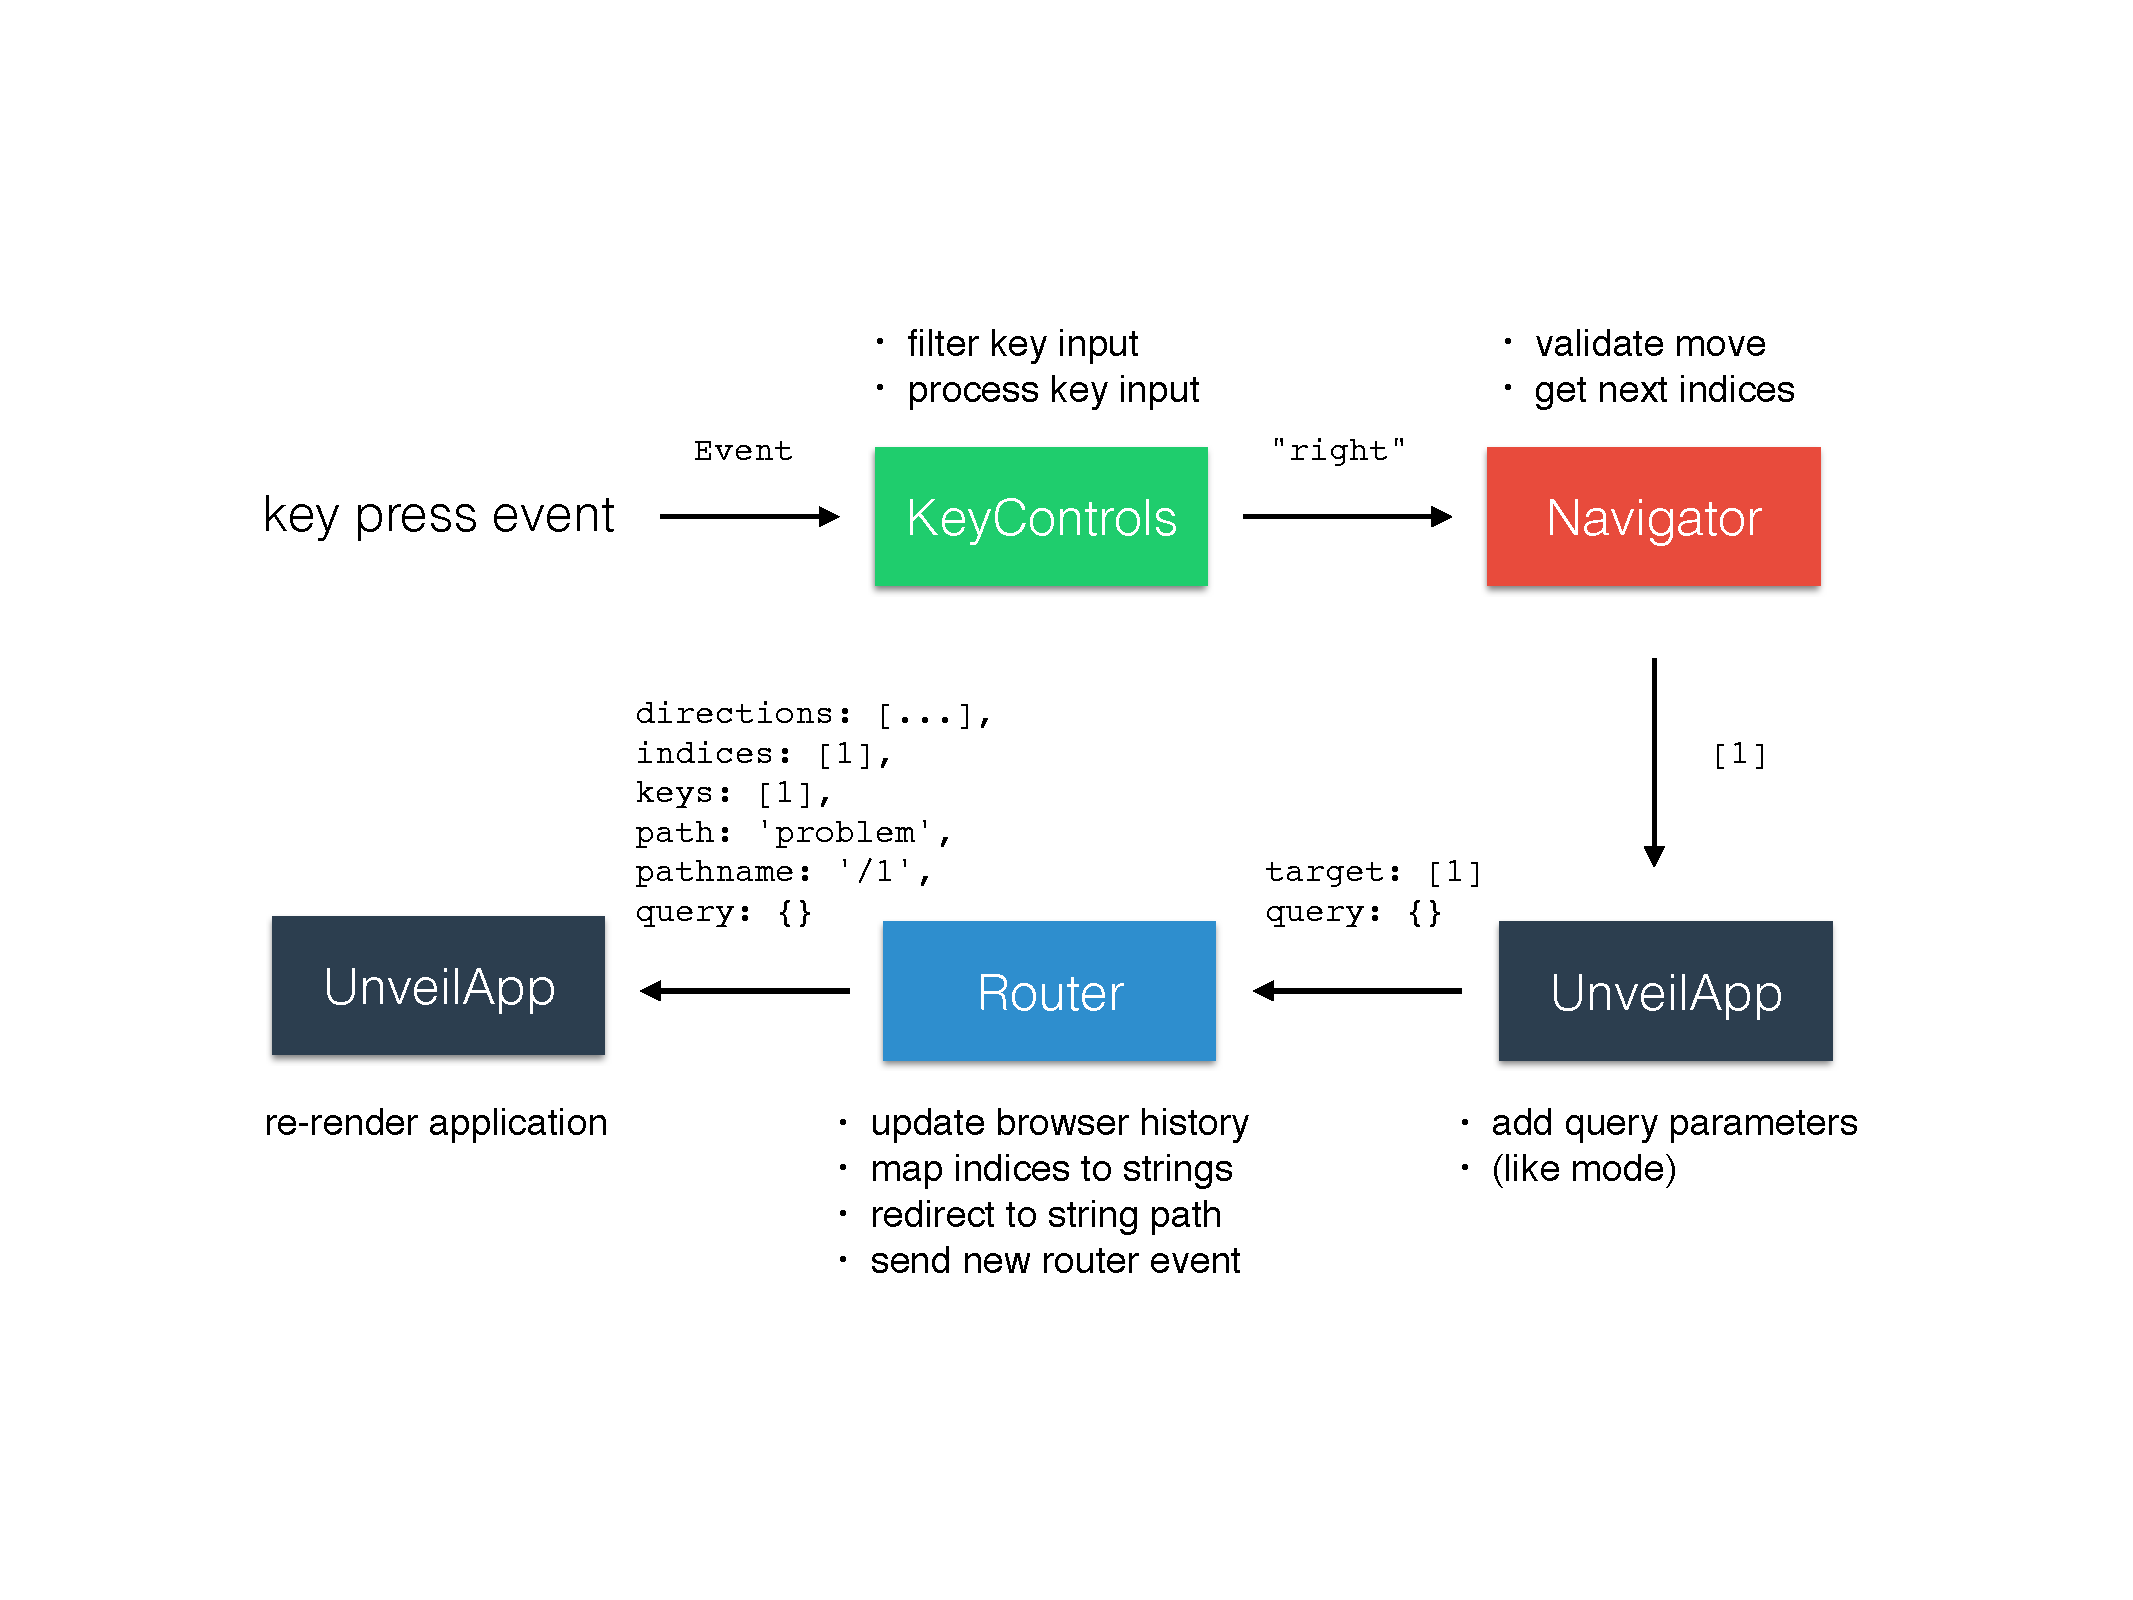
\includegraphics[width=.85\textwidth]{navigation}
\caption{Navigation pipeline from user's key press to re-render of the presentation. The monospaced text next to the arrows symbolises the data transmitted. \texttt{KeyControls} listen for key events and process them, to then send a navigation request to go \emph{right} to the \texttt{Navigator}. This component then maps the direction to the next slide's indices ($1$). \texttt{UnveilApp} then adds other information necessary for the \texttt{Router}, which then is responsible for updating the browser history, mapping the indices back to a human readable url and sending out a new router event. In the end \texttt{UnveilApp} receives this event and re-renders the presentation.}
\label{fig:implementation-technologies-unveil-navigation}
\end{figure}

%\subsection[socket.io]%
%             {socket.io%
%             \protect\footnote{\url{http://socket.io/}}}%
%\label{sec:implementation-architecture-socketio}
% problematic, talk about alternatives and problems in production, maybe even HTTP2
% e.g. safari conntection issues
% broadcasting functionality didn't quite work
% corporate firewalls can be a problem! big, in comparison to others

\section{Project Structure}
\label{sec:implementation-structure}
% A graphic explaining how the repos are built on top of each other would be great
% Which repos do I have and what do they include functionality-wise?
% explain why different repos and how they are all own npm packages that can easily be included in other projects

As the puropose of this project was not only to experiment with different ways of interacting with presentations using mobile devices, but also to create something worthwhile and contribute back to the vibrant open-source community, the project is enitrely open-source and separated into different repositories, which are all available on GitHub. These can be installed using npm, therefore allowing developers to rely only on the parts they really need.

\paragraph{Extended unveil.js:} As discussed in section \ref{sec:implementation-technologies-unveil}, the project is based on the library unveil.js. During the development of the project, certain parts of the base library did not offer the flexibility needed for easy extensibility and so several parts were adapted and new presentation logic was added. This happened in a fork of the original library, which will be examined in section \ref{sec:implementation-unveil}.

\paragraph{Network Synchronisation Layer:} The first library of direct importance for the interaction between speaker and audience through personal devices is \textit{unveil-network-sync}\footnote{\url{https://github.com/irisSchaffer/unveil-network-sync}}. This rather small library relies on unveil.js and is responsible for connecting the client and the server through web sockets and enables the synchronisation of the current slide displayed between speaker, audience and projector. The implementation of the features will be discussed in detail in section \ref{sec:implementation-network-sync}.

\paragraph{Interactive Extension:} As the name already suggests, this library is at the core of the present thesis: It includes a dedicated presenter for the speaker, implements the insertion of additional slides and subslides and by that allows the audience to share content with the presentation. The voting mechanism, as well as the creation of new votings on-the-fly, also live within this library. The repository, called \emph{unveil-interactive}\footnote{\url{https://github.com/irisSchaffer/unveil-interactive}} relies on unveil-network-sync for the socket-interaction. The interactive extension will be covered in section \ref{sec:implementation-interactive} of this chapter.

\paragraph{Server and Example Presentation:} The last repository connected to this thesis is \emph{unveil-client-server}\footnote{\url{https://github.com/irisSchaffer/unveil-client-server}}, which includes a simple server as well as a real-world example of a presentation, which was used in the intermediate thesis project presentation as part of the Interactive Media course IM690, on the 2\textsuperscript{nd}\xspace of February, 2016. In this chapter, a whole section was dedicated to the server (\ref{sec:implementation-server}), as well as to the example application (\ref{sec:implementation-client}), to separate concerns a bit more clearly and be able to conclude with a demonstration of how all parts discussed earlier play together in a final presentation.

\section{Extended unveil.js}
\label{sec:implementation-unveil}
% Add screenshots from biiiiiiig screen :)
The biggest adaptions and additions were necessary in the main component \texttt{UnveilApp}. A state subject was added to allow all components in the presentation to interact with the application. This subject receives an event with type and data and depending on this type starts a certain state change. Two of these state events are the \texttt{state/navigation:enable} and \texttt{state/navigation:disable} events, which set a state-variable \texttt{navigatable} to true or false. This variable is used in the controls to determine navigatability, therefore making it possible to keep the audience locked to a slide, e.g. during votings.
To make it possible for the audience to add subslides, as well as to dynamically add votings on-the-fly, another event is \texttt{state/slide:add}. It includes what slide to add (content), how (subslide or main slide) and where (under or after which slide). On occurence of this event, the slide-tree has to be re-built, the router and navigator re-started and the whole presentation re-rendered, which the library also had to be prepared for.

\begin{figure}
\centering
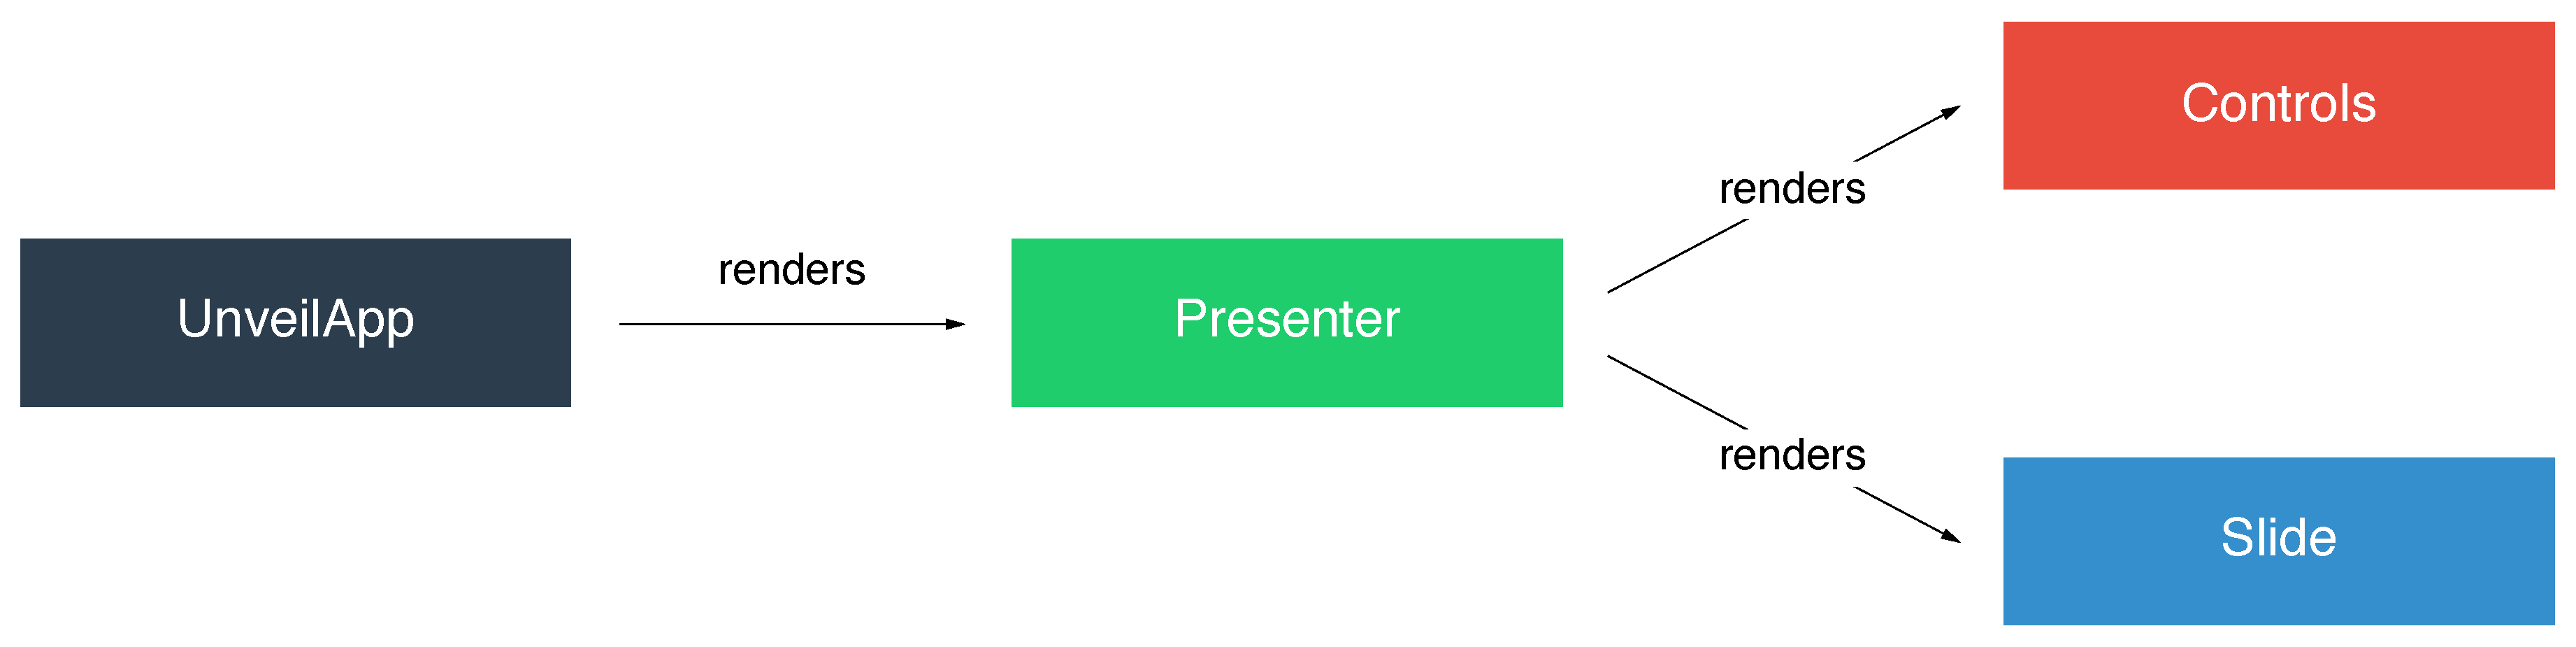
\includegraphics[width=.5\textwidth]{render-pipeline}
\caption{Overview over the render-flow of the application in the extended version of unveil.js. \texttt{UnveilApp} renders the presenter, which then takes care of rendering the (current) slide and all controls.}
\label{fig:implementation-unveil-render-pipeline}
\end{figure}

Another adaption in \texttt{UnveilApp} is the introduction of the \texttt{context} object: Additionally to state and properties, there is a third way of communicating between components in React, called \emph{context}. Instead of having to pass properties from one nested component to the other, every child component can access the context of its parents. The navigator, needed in the controls, was formerly passed from \texttt{UnveilApp} to the controls through several layers. Using context, \texttt{UnveilApp} now defines a number of different variables which are available through context, including current slide and router state, navigator, mode and the state subject discussed in the last paragraph. This makes it easy for new controls and presenters to access the data they need without other layers knowing about them or having to define them.
This adaption was partly due to a change in the render hierarchy: Formerly, \texttt{UnveilApp} itself rendered the presenter (which rendered the current slide) and the controls. However, the presenter needs to be able to also control the rendering of controls (see figure \ref{fig:implementation-unveil-render-pipeline}), adding another layer between the rendering of controls and \texttt{UnveilApp}.

Another part that was added to the unveil.js base library is the \texttt{Notes} component. It allows adding speaker notes to each slide (see program \ref{prog:implementation-technologies-react}). These, however, are not rendered by the slide, but by the presenter, as will be shown in section \ref{sec:implementation-interactive}. One more important new feature is the possibility to configure the next slide in a certain direction (left/right/up/down) and therefore allow for jumping into different branches of the presentation, thus making a presentation even more interactive. The following code, for example
%
\begin{JsCode}
  <Slide name="start" left={[0]}>
    ...
  </Slide>
\end{JsCode}
%
means a navigation \emph{left} (left arrow key pressed, swipe left etc.) will not go to the previous slide defined in the slide-tree, but rather jump to the first slide (of index $0$).


\section{Network Synchronisation Layer}
\label{sec:implementation-network-sync}
% Mention problems with socket io here! --> Corporate firewalls can block socket io entirely, etc.
As mentioned before, the network synchronisation layer is responsible for the communcation between server and client using web sockets. These are created with socket.io, a library which also provides fallbacks for browsers that do not support web sockets yet. However, this library also has a few drawbacks, especially when it comes to corporate networks. As Rob Britton describes in \cite{socketio-problems}, socket.io seems to have problems getting through firewalls and can be blocked by some anti virus software.
Because mobile browser support is essential for this project, I decided to still use this library.

The setup of the socket is simple: one helper function, called \texttt{createSocket} is called in the main entry point of the application to configure which server to connect to:
%
\begin{JsCode}
import { createSocket } from 'unveil-network-sync'
createSocket('46.101.166.172:9000')
\end{JsCode}
%
This function creates the socket and returns it as a singleton, so every component uses the same connection. To make importing even easier, there is another helper, called \texttt{SocketIO} which dan be importet directly and internally calls \texttt{createSocket} to retrieve the singleton:
%
\begin{JsCode}
import { SocketIO } from 'unveil-network-sync'
\end{JsCode}
%

These sockets can then be used to listen to events or to emit them (see program \ref{prog:implementation-network-sync-navigation-receiver}) Like the state subject events, the socket.io events used in this library follow the naming convention of scoping the object targeted in by the event separated by slashes, followed by a colon and the name of the action, e.g. \texttt{state:change} or \texttt{state/slide/voting:start}.

\begin{program}
\caption{Shortened version of \texttt{NavigationReceiver}. First the inherited context properties are set up, then an observable waiting for \texttt{state:change} events from the socket is created. If the incoming request is not the currently displayed slide, the navigator will be pushed a new value.}
\label{prog:implementation-network-sync-navigation-receiver}
\begin{JsCode}
// imports...

export default class NavigationReceiver extends React.Component {
  static contextTypes = {
    navigator:   React.PropTypes.object.isRequired,
    routerState: React.PropTypes.object.isRequired
  }

  componentDidMount () {
    this.observable = Observable.fromEvent(SocketIO, 'state:change')
      .filter((e) => !this.context.routerState.indices.equals(e))
      .subscribe(this.props.navigator.next)
  }
  ...
}
\end{JsCode}
\end{program}
%
The second responisbilty of this library is synchronising the navigation state of the presentation between speaker and audience. To do this, two controls, \texttt{NavigationSender} and \texttt{NavigationReceiver} were implemented. As the names already say, the sender broadcasts the state update, while the receiver is waiting for state updates and starts the navigation process. The latter is used in all modes (default, speaker and projector), whereas the sender is only added to the speaker mode. To make sure the sender does not end up in an infinite loop of sending and receiving its own state changes, the last received state is stored and only navigation events going to a different slide are processed further.

This mechanism, though relatively simple, already enables the audience to follow the presentation, the speaker to use his/her phone as a remote control and any number of projectors to be controlled by the speaker.

\section{Interactive Extension}
\label{sec:implementation-interactive}
The interactive library includes several parts which will be discussed here: a speaker presenter (section \ref{sec:implementation-interactive-speaker-presenter}) as well as different components connected to sharing media (section \ref{sec:implementation-interactive-media}) and voting (section \ref{sec:implementation-interactive-voting}). Additionally controls handling the \texttt{state:initial} event were implemented to redirect new listeners to the current slide in the presentation.

\subsection{Speaker Presenter}
\label{sec:implementation-interactive-speaker-presenter}

The speaker presenter, like the normal presenter, is responsible for rendering controls and slides. In speaker mode, where this presenter is used, notes as well as the upcoming slides (right and down) are also shown (see figure \ref{fig:implementation-interactive-speaker-presenter}).
This means the presenter has to find these next slides, using the router's information about the navigatable directions, and render them in a designated area. To make the presenter view usable on mobile devices, special attention was paid to mobile stylesheets (see figure \ref{fig:implementation-interactive-mobile} (b)). This ensures that everything is big enough to be readable and all buttons are clickable.

\begin{figure}
\centering
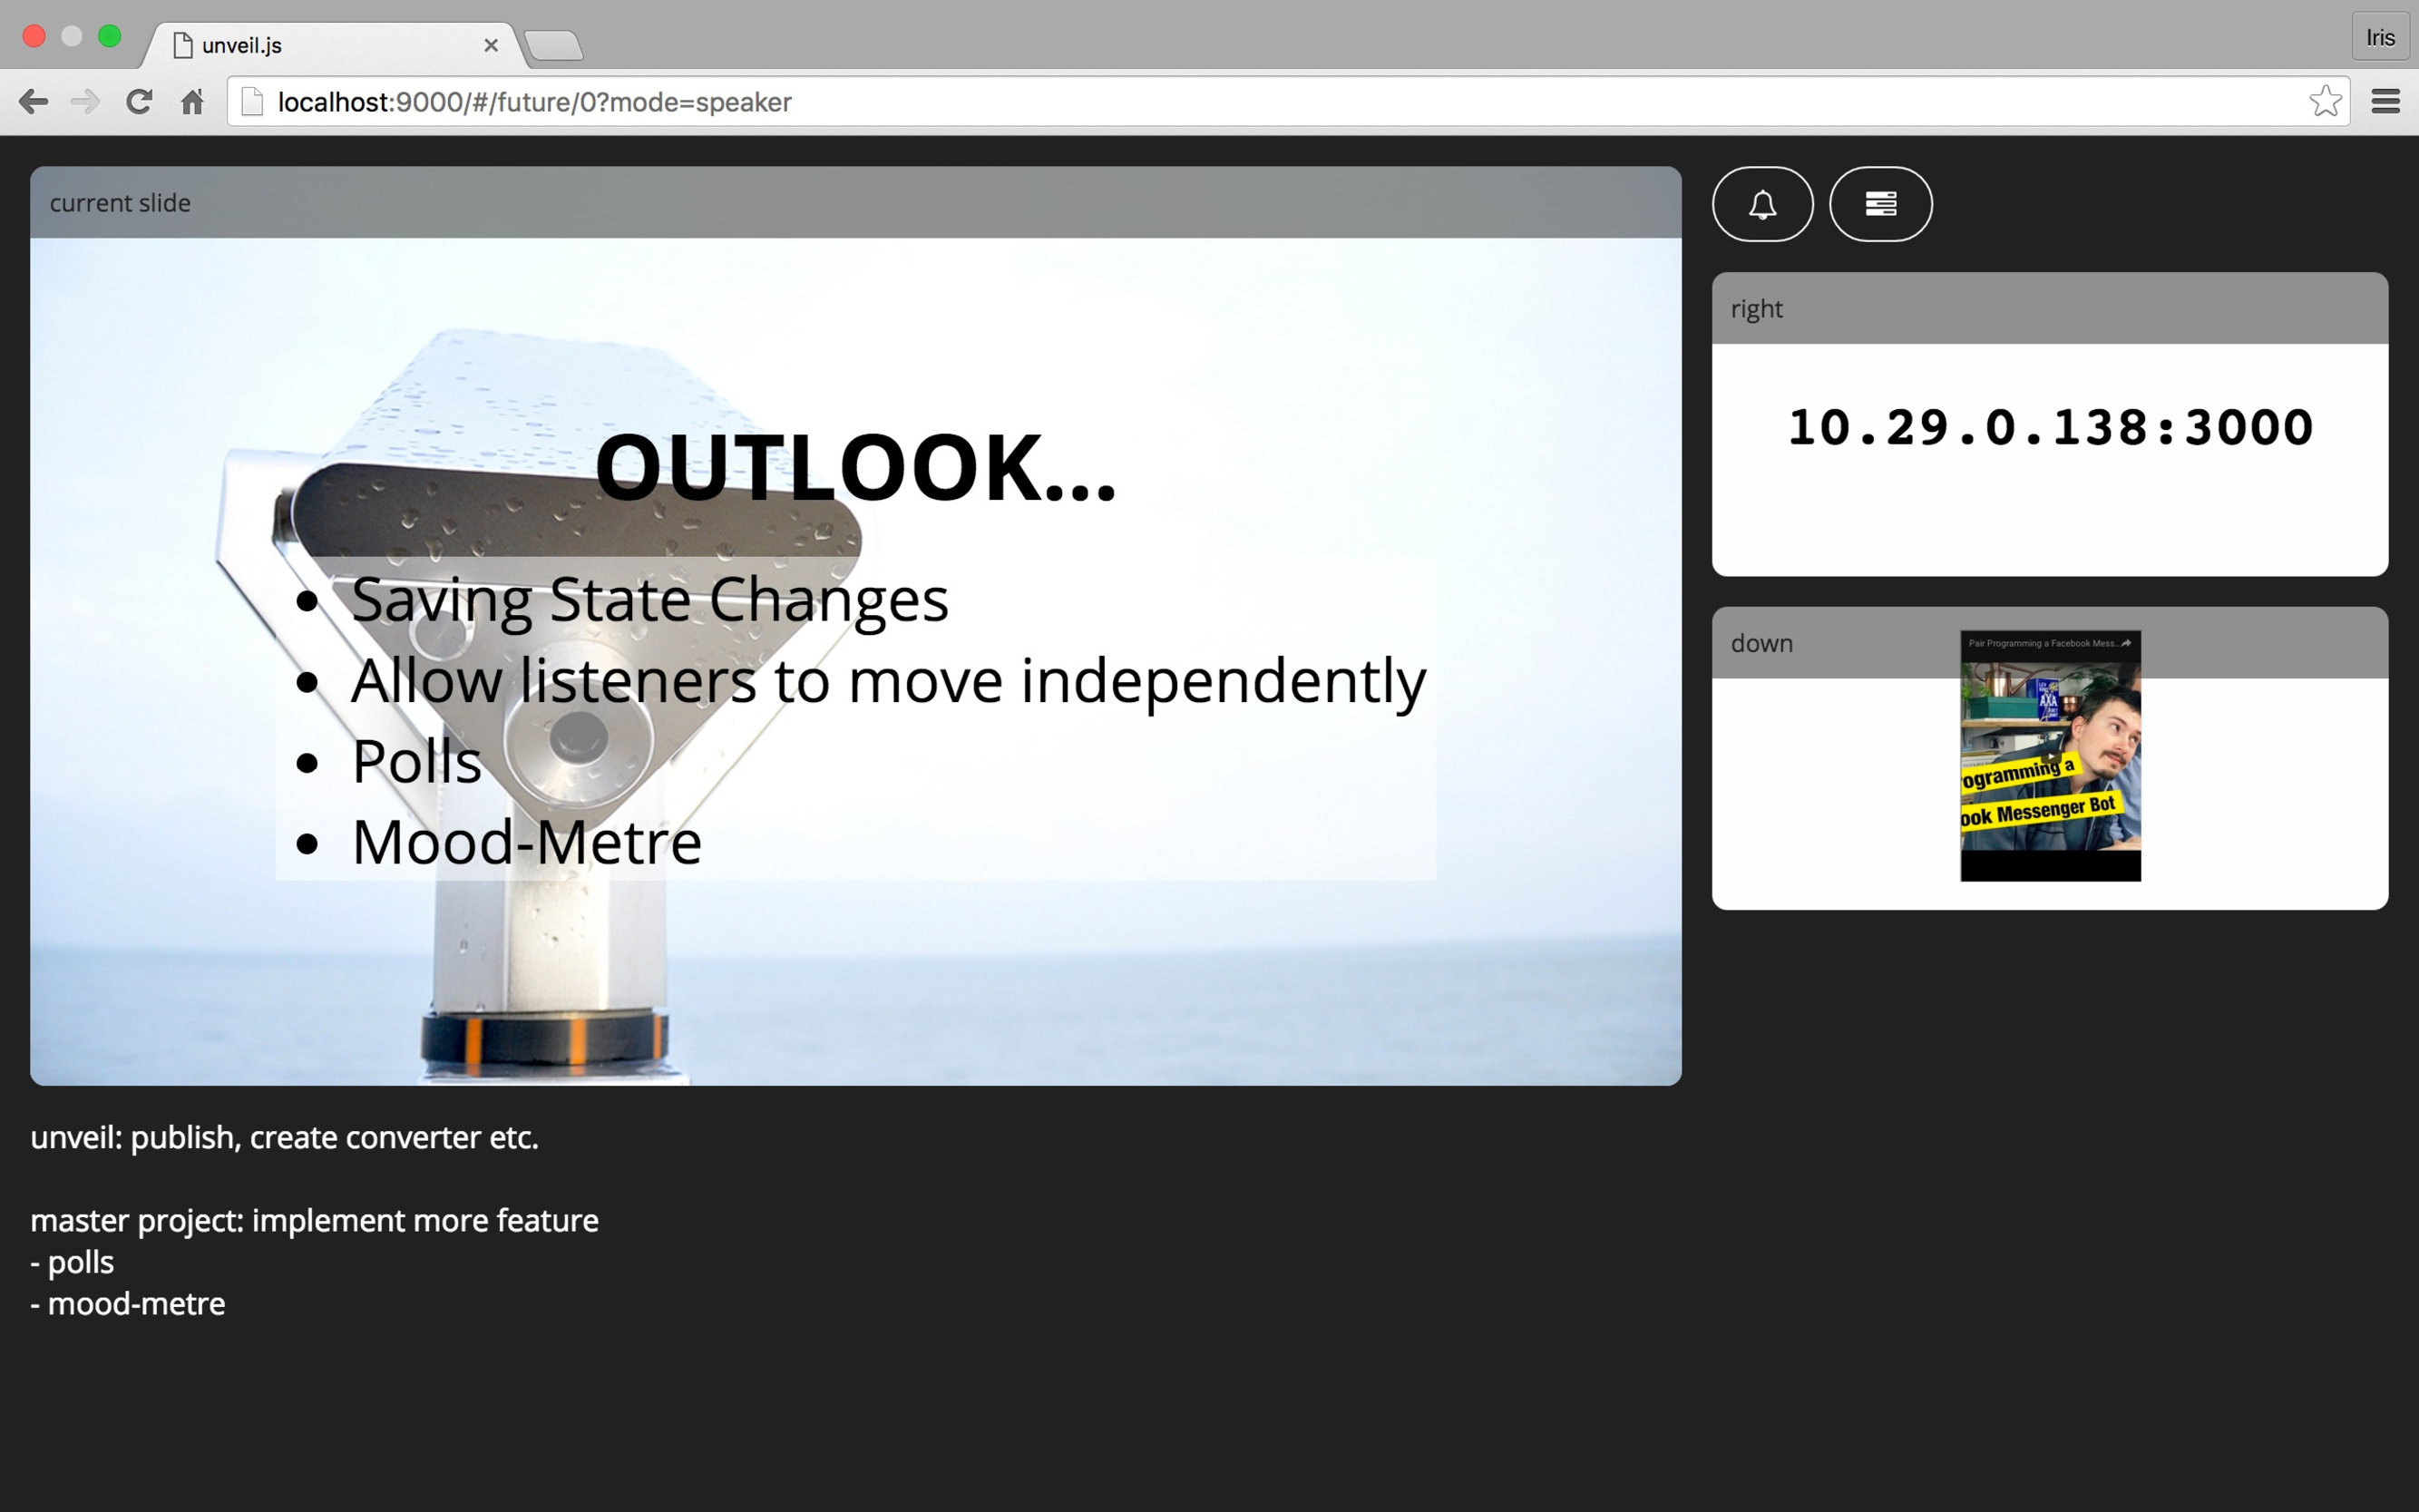
\includegraphics[width=.65\textwidth]{media-accepted-screenshot}
\caption{Screenshot of the speaker presenter with the current main slide, the upcoming slide to the right, available actions (muting and adding votings) and speaker notes.}
\label{fig:implementation-interactive-speaker-presenter}
\end{figure}

\begin{figure}
\centering\small
\begin{tabular}{cccc}
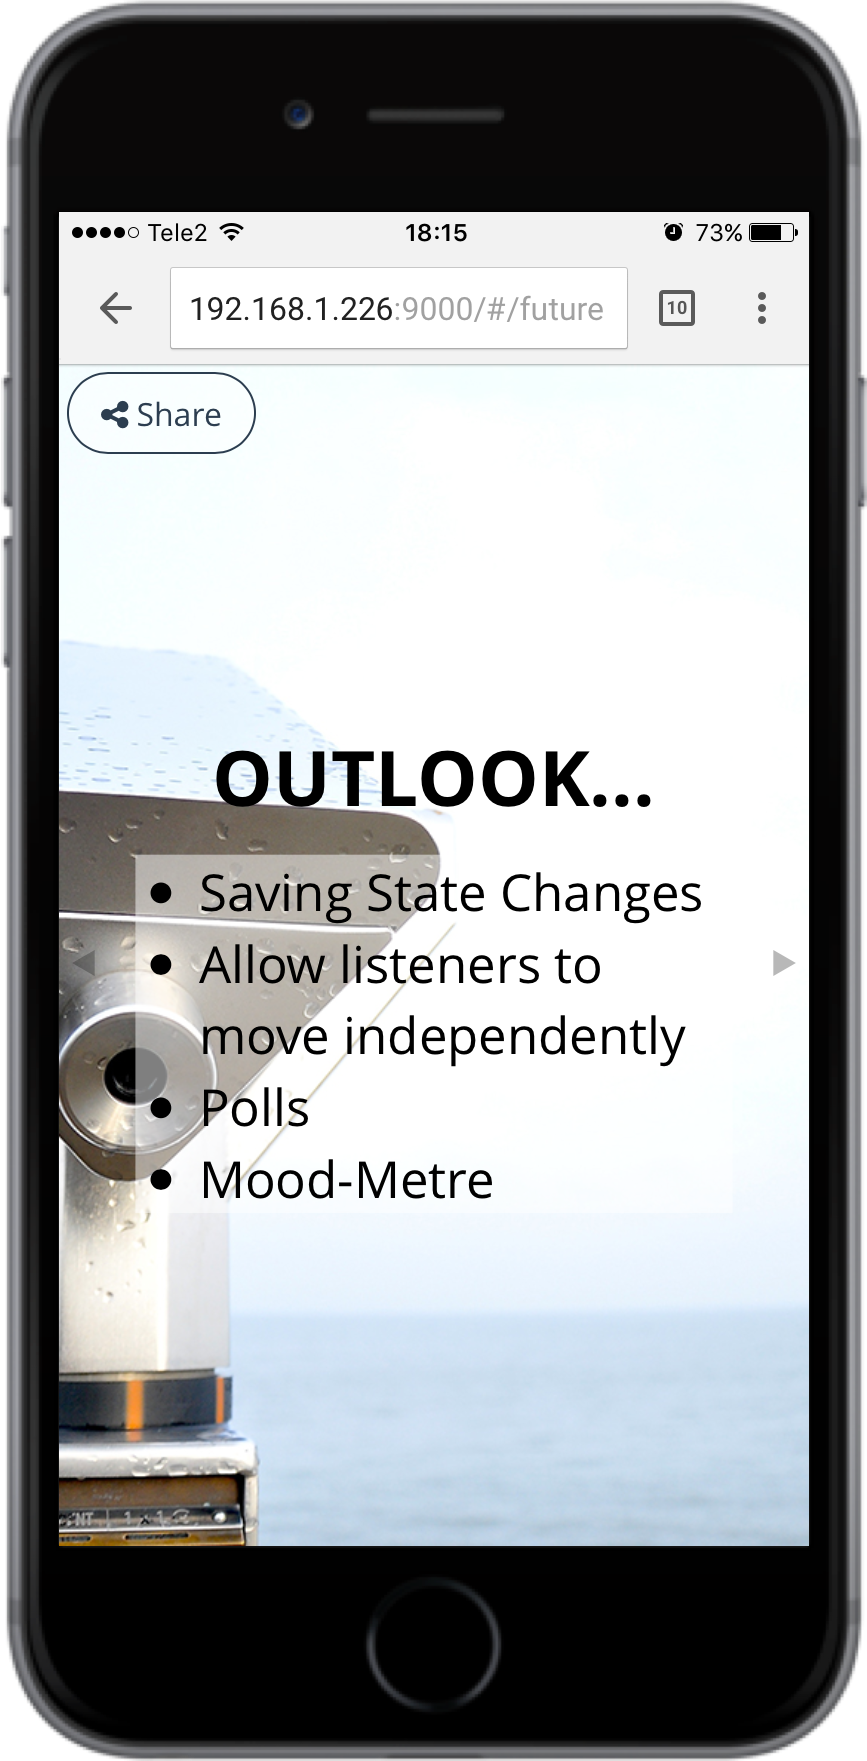
\includegraphics[width=.2\textwidth]{presentation-screenshot-mobile} &
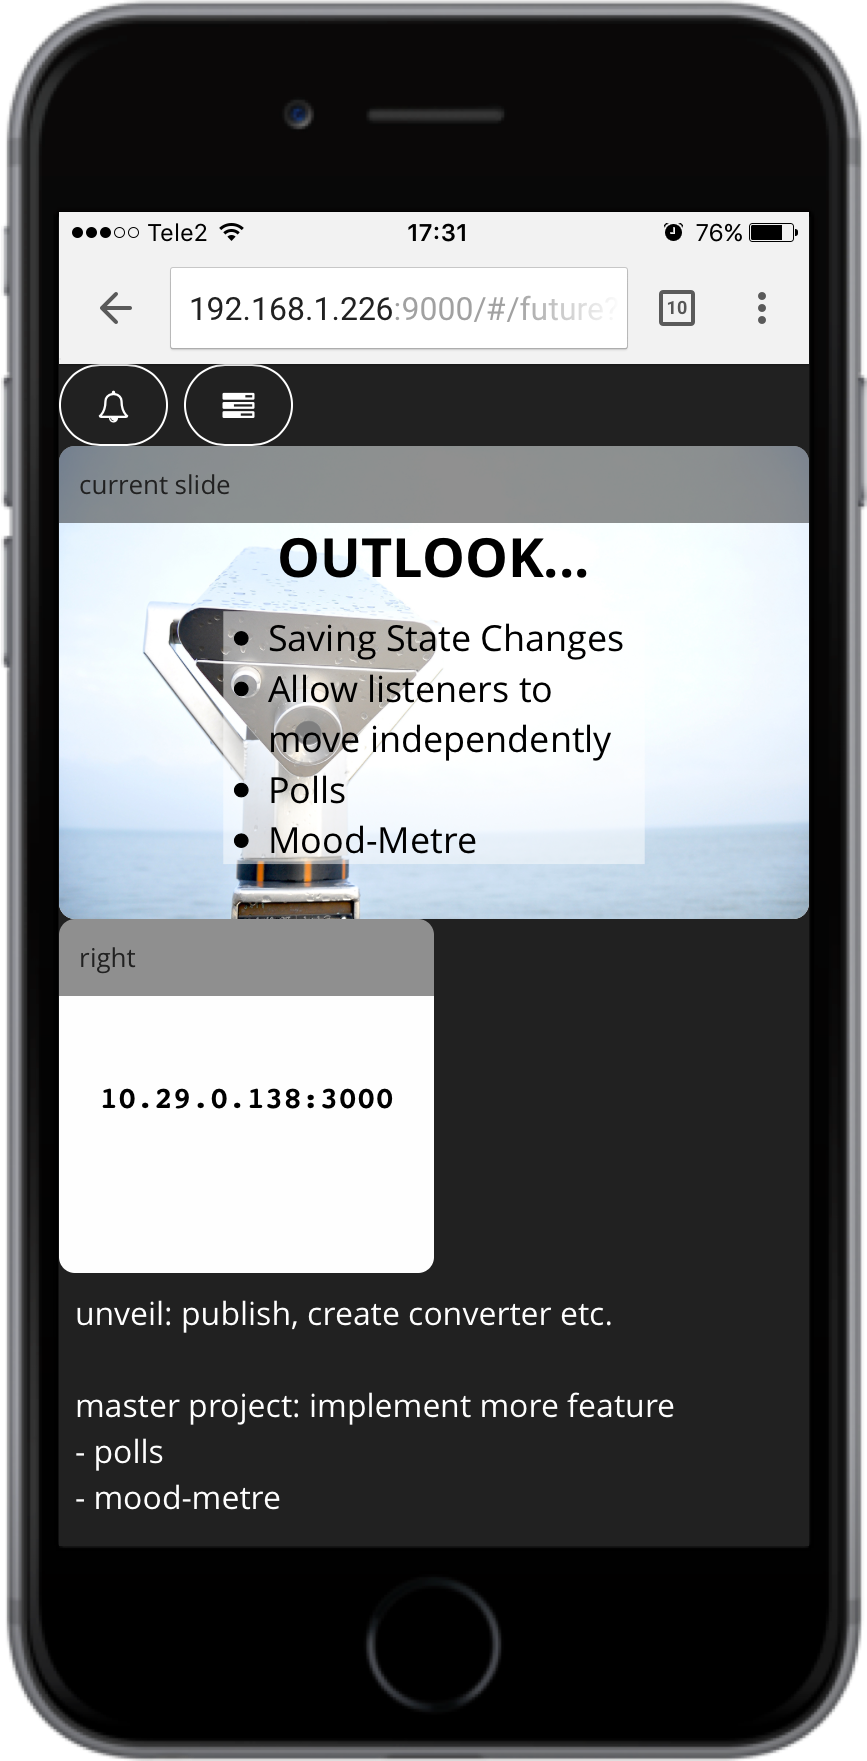
\includegraphics[width=.2\textwidth]{speaker-presenter-screenshot-mobile} &
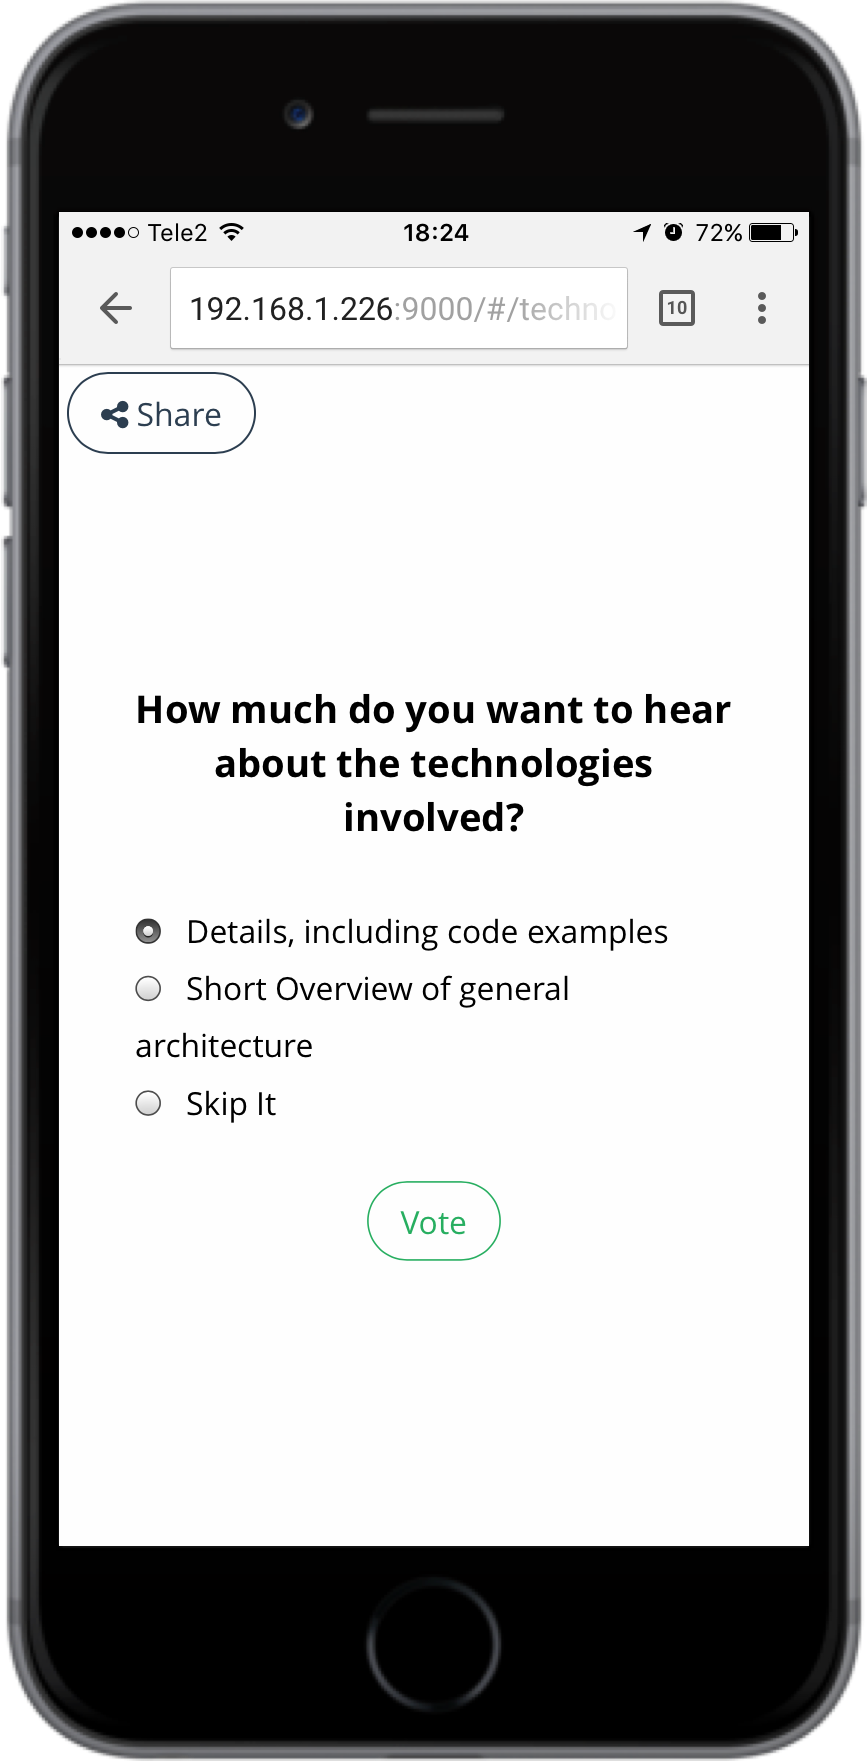
\includegraphics[width=.2\textwidth]{voting-screenshot-mobile} &
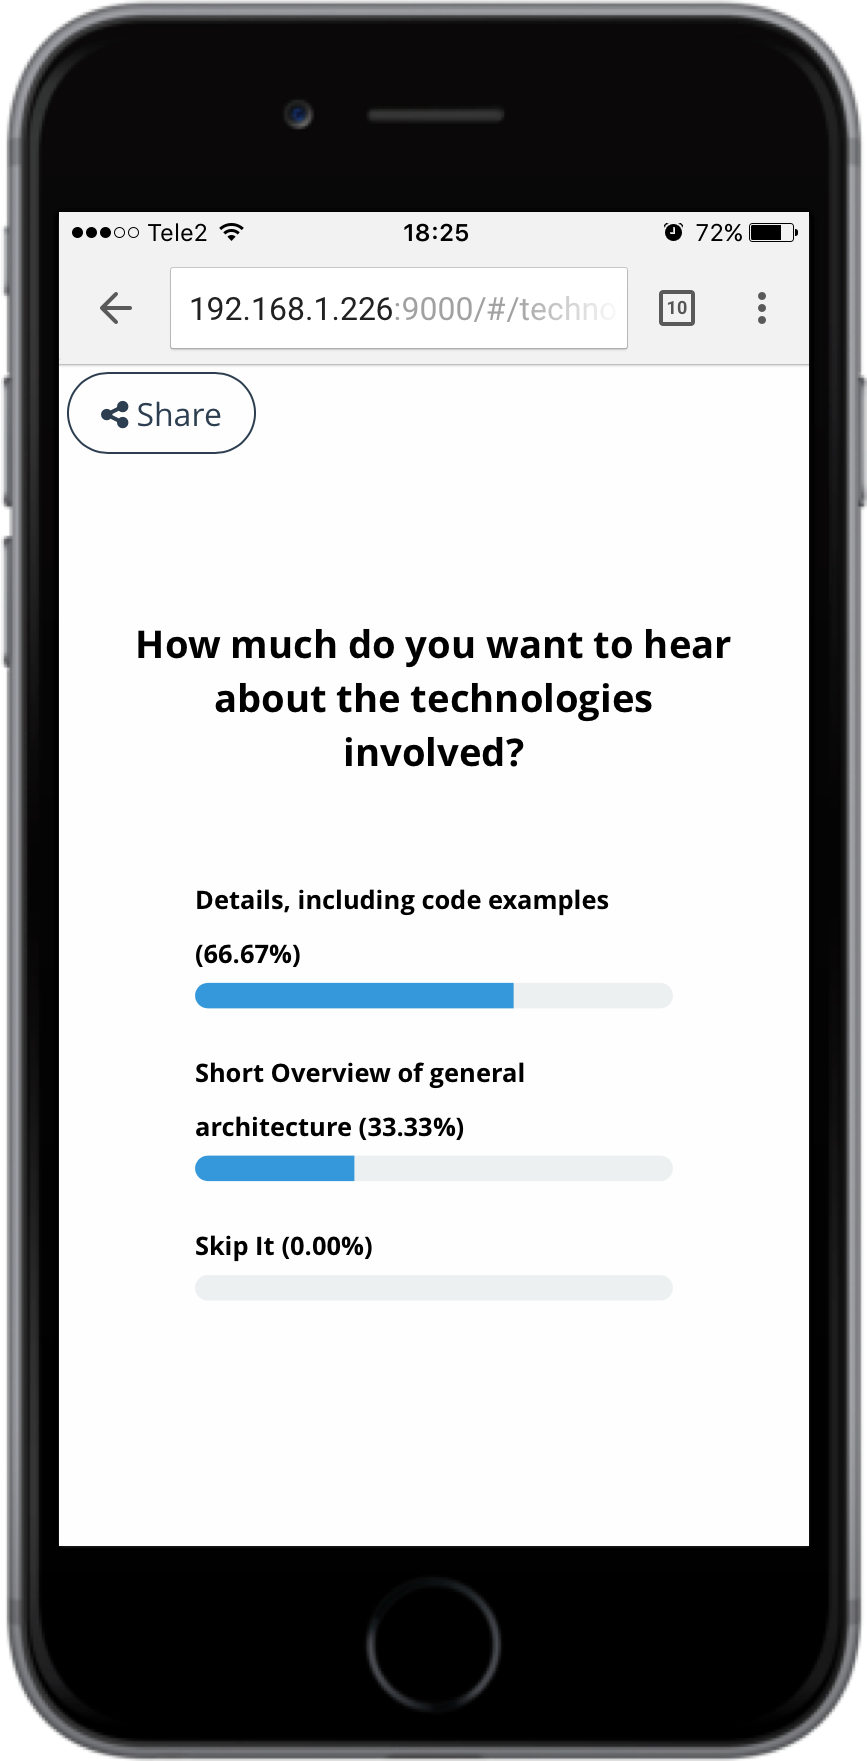
\includegraphics[width=.2\textwidth]{voting-results-screenshot-mobile} \\
(a) & (b) & (c) & (d)
\end{tabular}
\caption{Mobile view of a presentation slide in (a) default mode and (b) speaker mode as well as (c) voting view before voting and (d) voting view after voting. Mind the share button in the left upper corner in (a) as well as the buttons to mute content requests and create votings in (b).}
\label{fig:implementation-interactive-mobile}
\end{figure}

\subsection{Media}
\label{sec:implementation-interactive-media}
Another responsibility of the interactive extension is the possibility for audience members to share content with the presentation. For this to work, three different controls were created: \texttt{MediaSender}, \texttt{MediaReceiver} and \texttt{MediaAcceptor}. The sender is used in the default mode so users can share their content (see figure \ref{fig:implementation-interactive-media} (a)), the acceptor is enabled in speaker mode, to accept or reject incoming media (see figure \ref{fig:implementation-interactive-media} (b)) and the receiver in the end handles the creation of a new slide if the content was accepted and is therefore necessary in all modes. As incoming content requests could disrupt the presentation flow and distract the speaker, an option to mute the requests was built into the application. If the \emph{do not disturb} mode is turned on, slides will silently be added as subslides, without causing the acceptor modal to open. This way the audience' additions can be re-visited after the end of the presentation. Generally, this feature can be used to either post a link to an interesting picture, website or even youtube video, or also as text input, for example to add a comment or a question regarding a certain slide. This works through the introduction of the presentation components \texttt{Media} and \texttt{IFrame}, which, depending on the shared content, render an image-tag, blockquote or IFrame. The differentiation of these is carried out with regular expressions, as the following to check if the content is the link to an image:
\begin{JsCode}
isImg (str) {
  let imgRegex = new RegExp(/\.(jpe?g|png|gif|bmp)$/i)
  return imgRegex.test(str)
}
\end{JsCode}

As far as the implementation of the controls is concerned, these ones are the first ones discussed in the present thesis makeing use of the \texttt{render()} method. It is used to output the \emph{share} button in the left upper corner in default mode (see figure \ref{fig:implementation-interactive-mobile} (a)) as well as the share modal opened when clicking on said button (see figure \ref{fig:implementation-interactive-media} (a)). The same happens in the \texttt{MediaAcceptor}, which uses the \texttt{render()} method to display the \emph{mute} button shown in figure \ref{fig:implementation-interactive-speaker-presenter} as well as the modal for accepting media (see figure \ref{fig:implementation-interactive-media} (b)).

These are also the first controls using state: in the sender a click on the share button sets the state variable \texttt{sharingMode} to \texttt{true} and through that enables the rendering of the modal. In the acceptor an array of \texttt{requests} is filled as new content is shared and emptied again, as the speaker accepts or denies them.

On event level, the socket events \texttt{state/slide/add:accept} and \texttt{state/ slide:add} are included in the process of sharing new content, in the end an unveil state event of type \texttt{state/slide:add} lets \texttt{UnveilApp} create the new slide and add it to the slide tree. The whole flow is outlined in details in figure \ref{fig:implementation-interactive-media-pipeline}.

\begin{figure}
\centering\small
\begin{tabular}{cc}
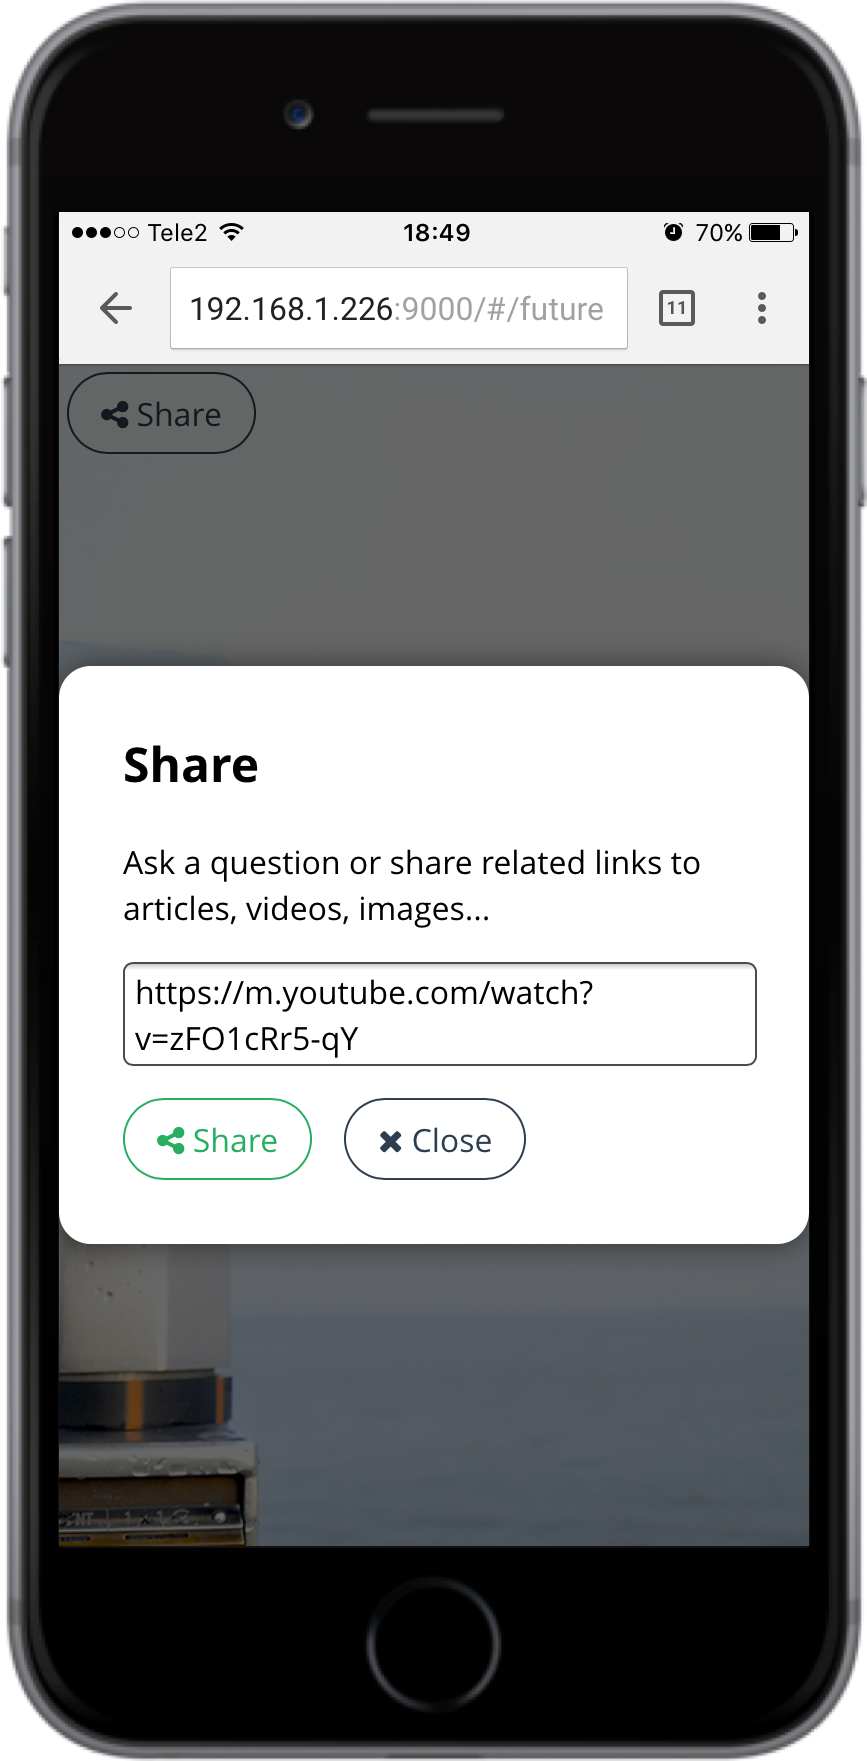
\includegraphics[width=.2\textwidth]{media-screenshot-mobile}
 &
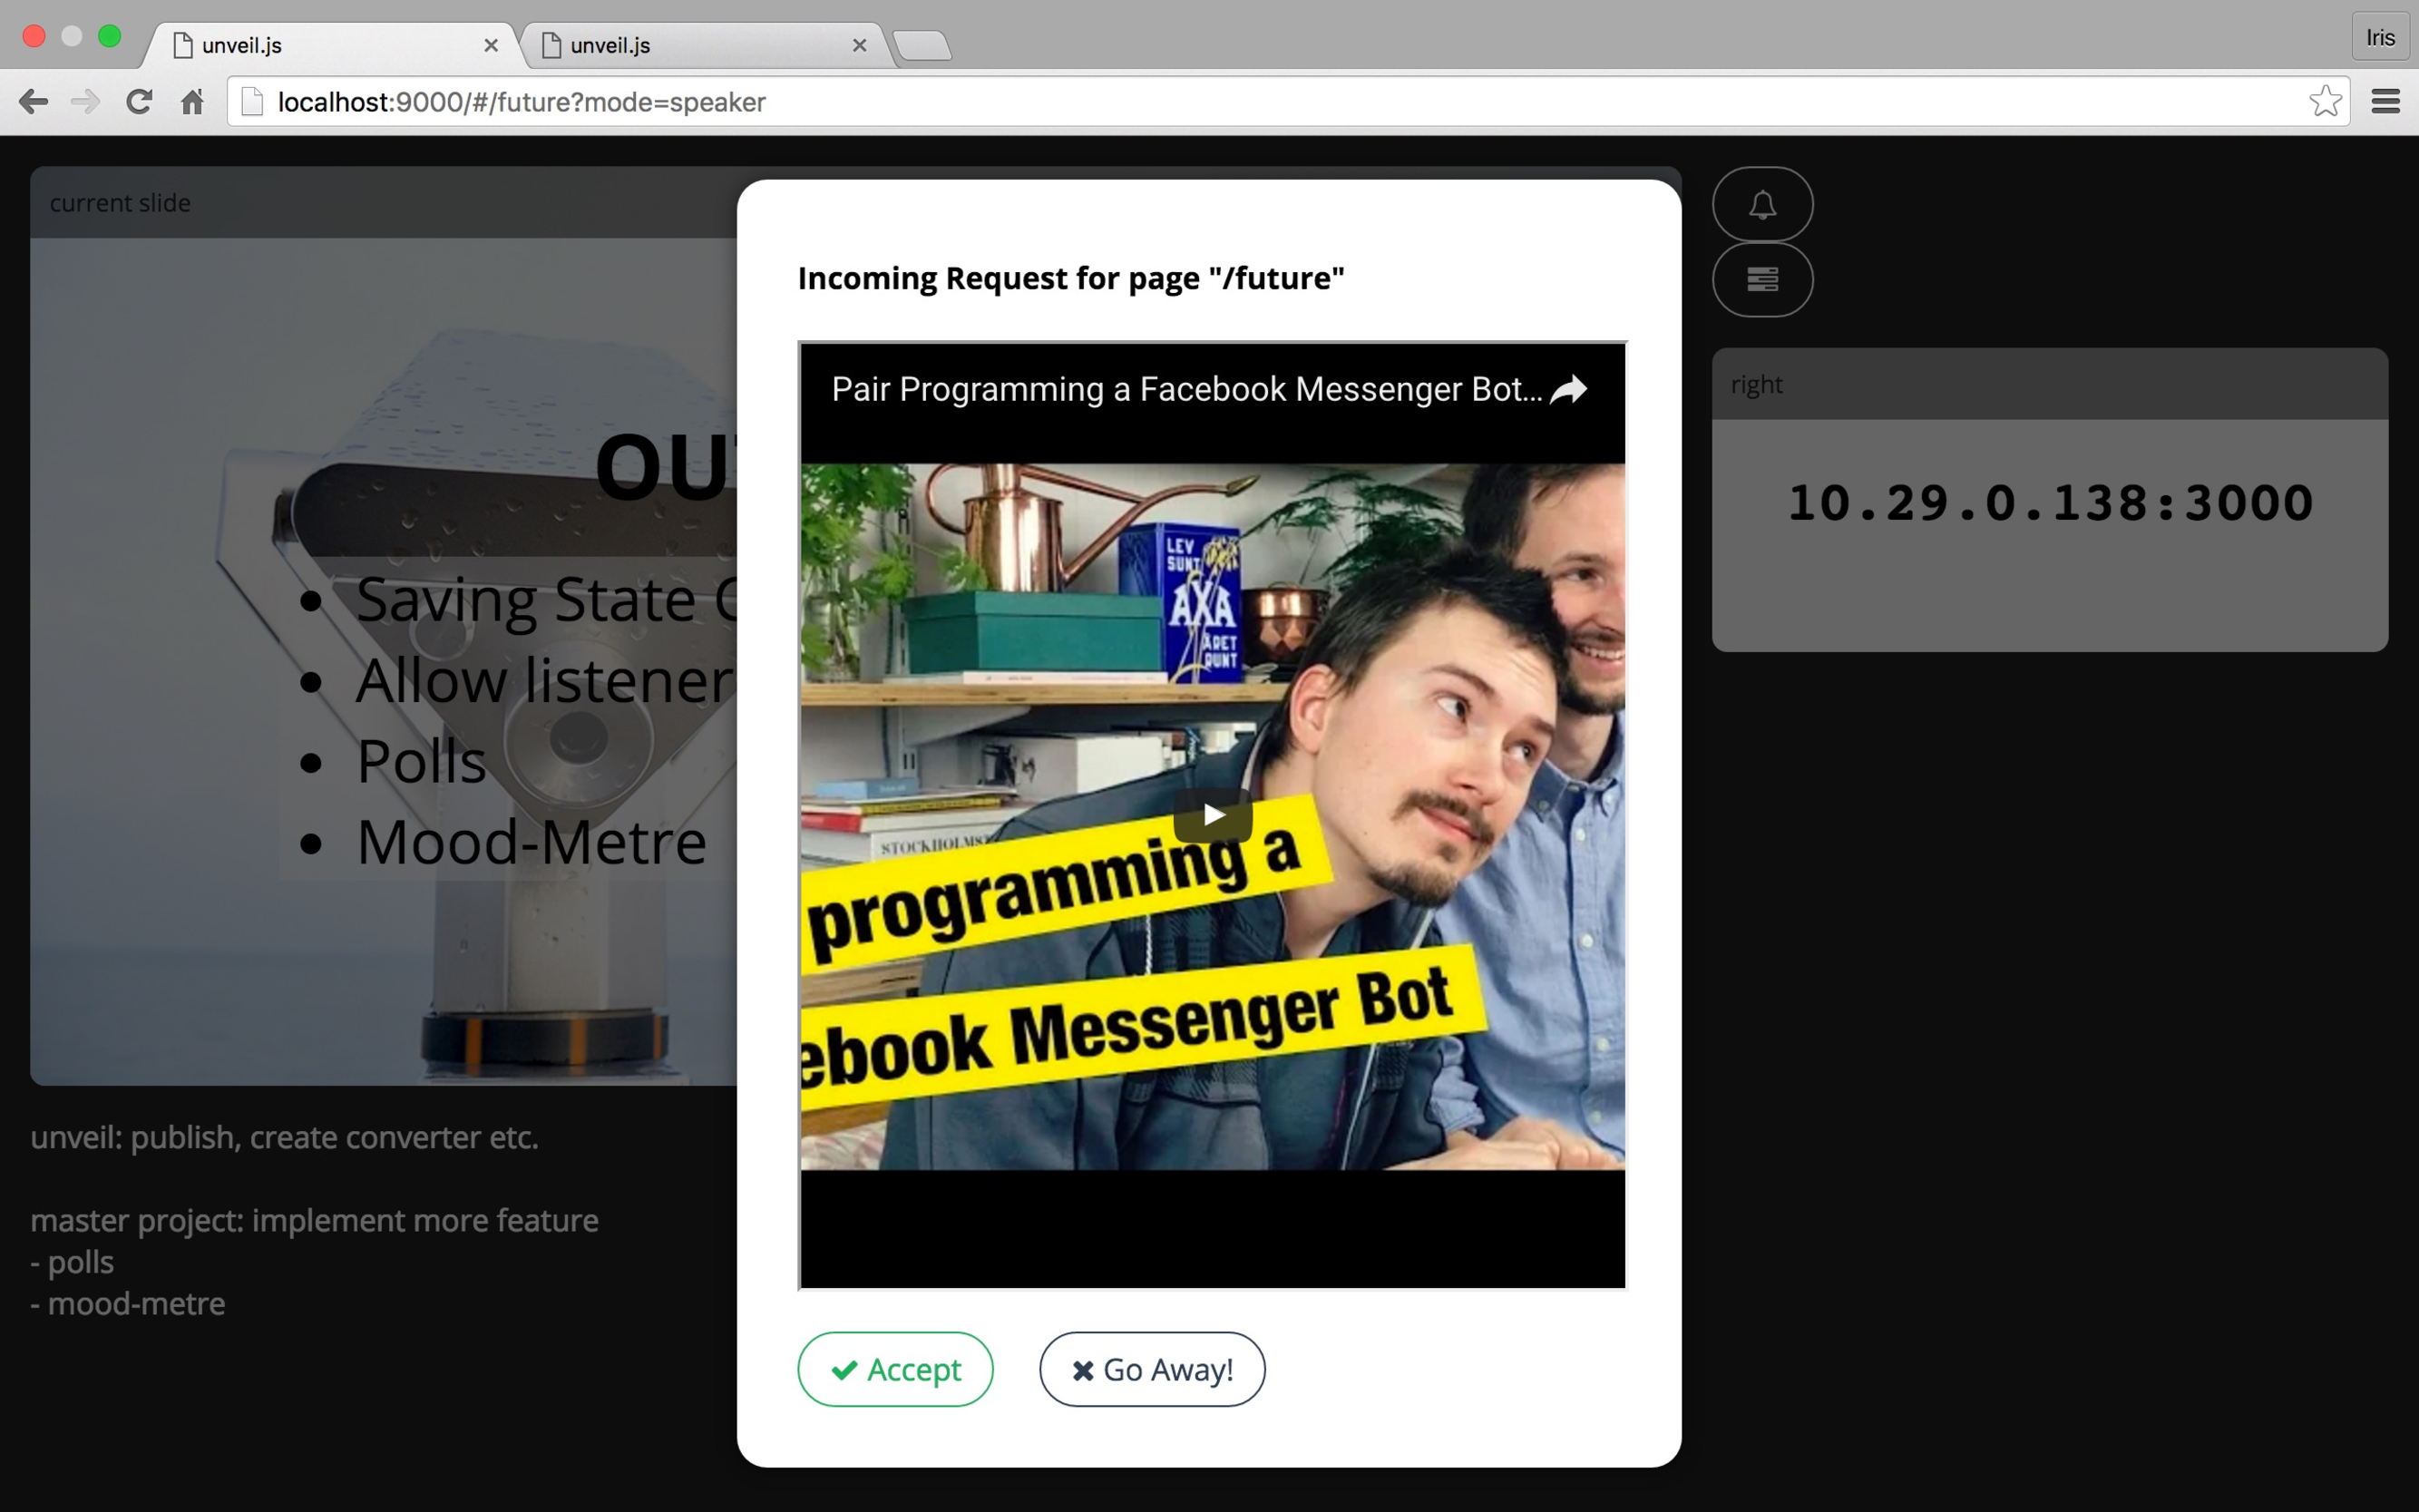
\includegraphics[width=.65\textwidth]{media-acceptor-screenshot} \\
(a) & (b)
\end{tabular}
\caption{Screenshots of sharing content. (a) media sender on mobile phone shares youtube link (b) speaker receives content request.}
\label{fig:implementation-interactive-media}
\end{figure}

\begin{figure}
\centering
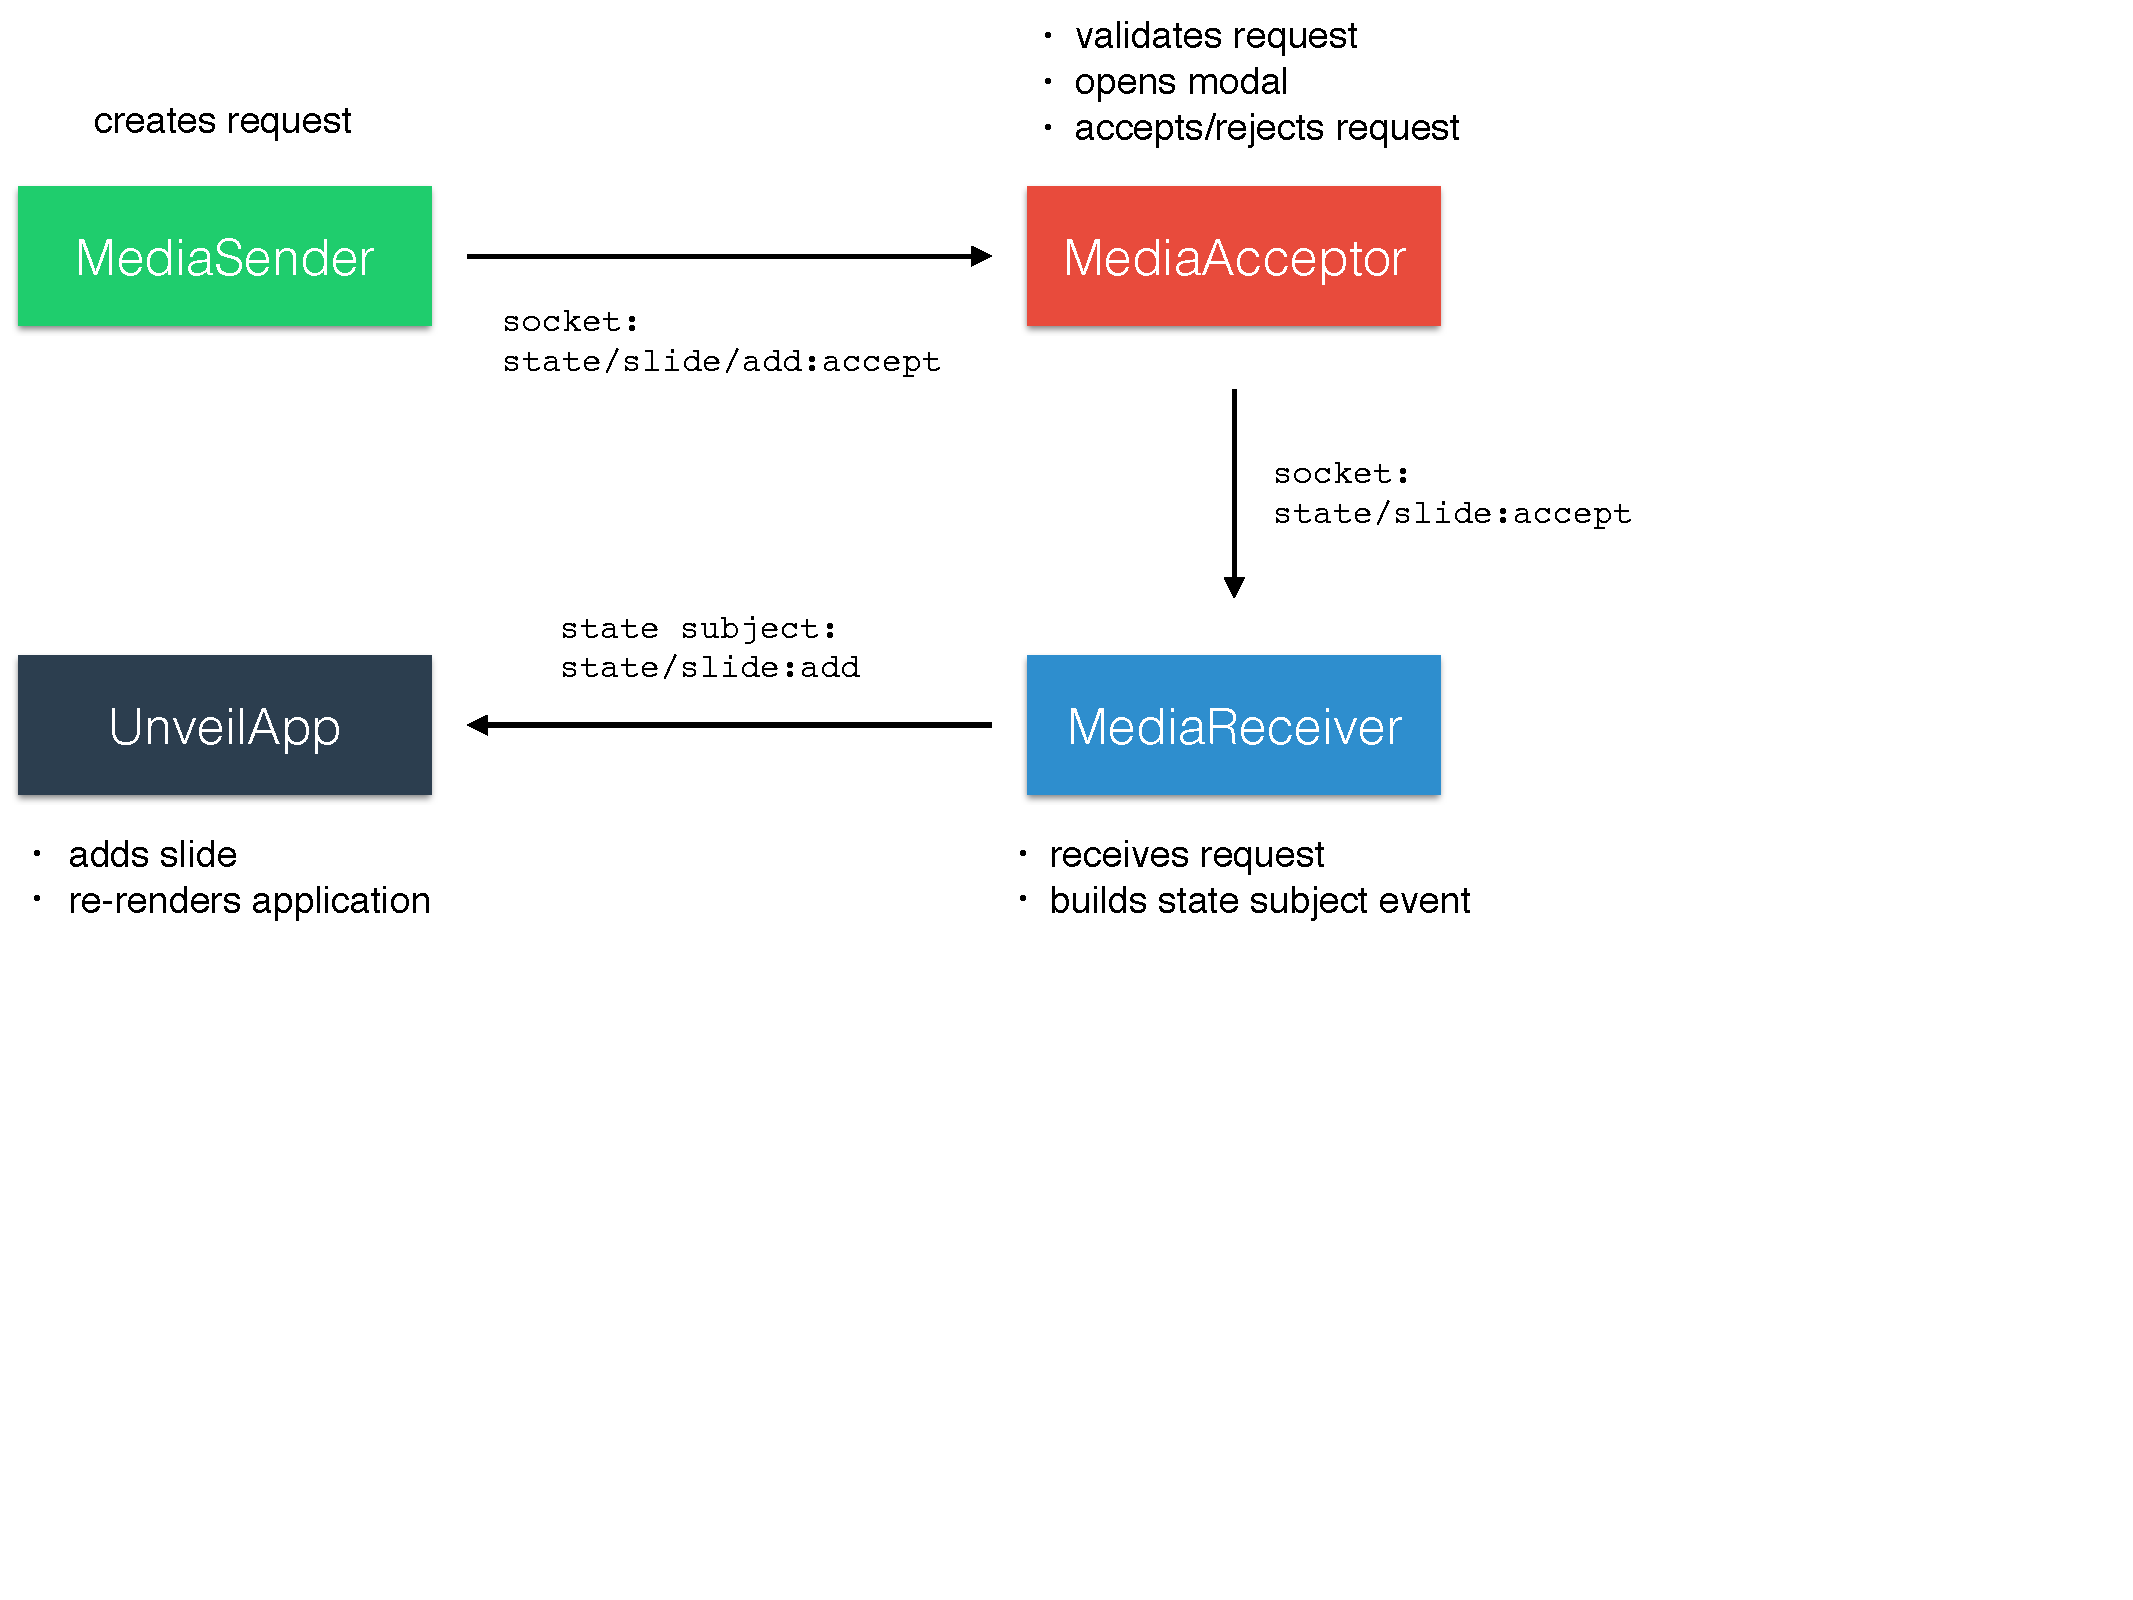
\includegraphics[width=.8\textwidth]{media-pipeline}
\caption{Flow of adding content, monospaced text symbolises type and name of events. First the \texttt{MediaSender} of the default mode sends a request, which the speaker mode's \texttt{MediaAcceptor} listens to. If the request is accepted by the speaker or requests are muted, another socket event is broadcast, which the \texttt{MediaReceiver} waits for. This component is enabled in all modes and emits the state subject event to add a new slide, which \texttt{UnveilApp} reacts to.}
\label{fig:implementation-interactive-media-pipeline}
\end{figure}

\subsection{Voting}
\label{sec:implementation-interactive-voting}

The last group of components connected to the interactive extension covered in this chapter allow speakers to create votings (both during in the preparation of the presentation and on-the-fly as shown in figure \ref{fig:implementation-interactive-voting}) and members of the audience to vote (see figure \ref{fig:implementation-interactive-mobile} (c) and (d)).

\begin{figure}
\centering
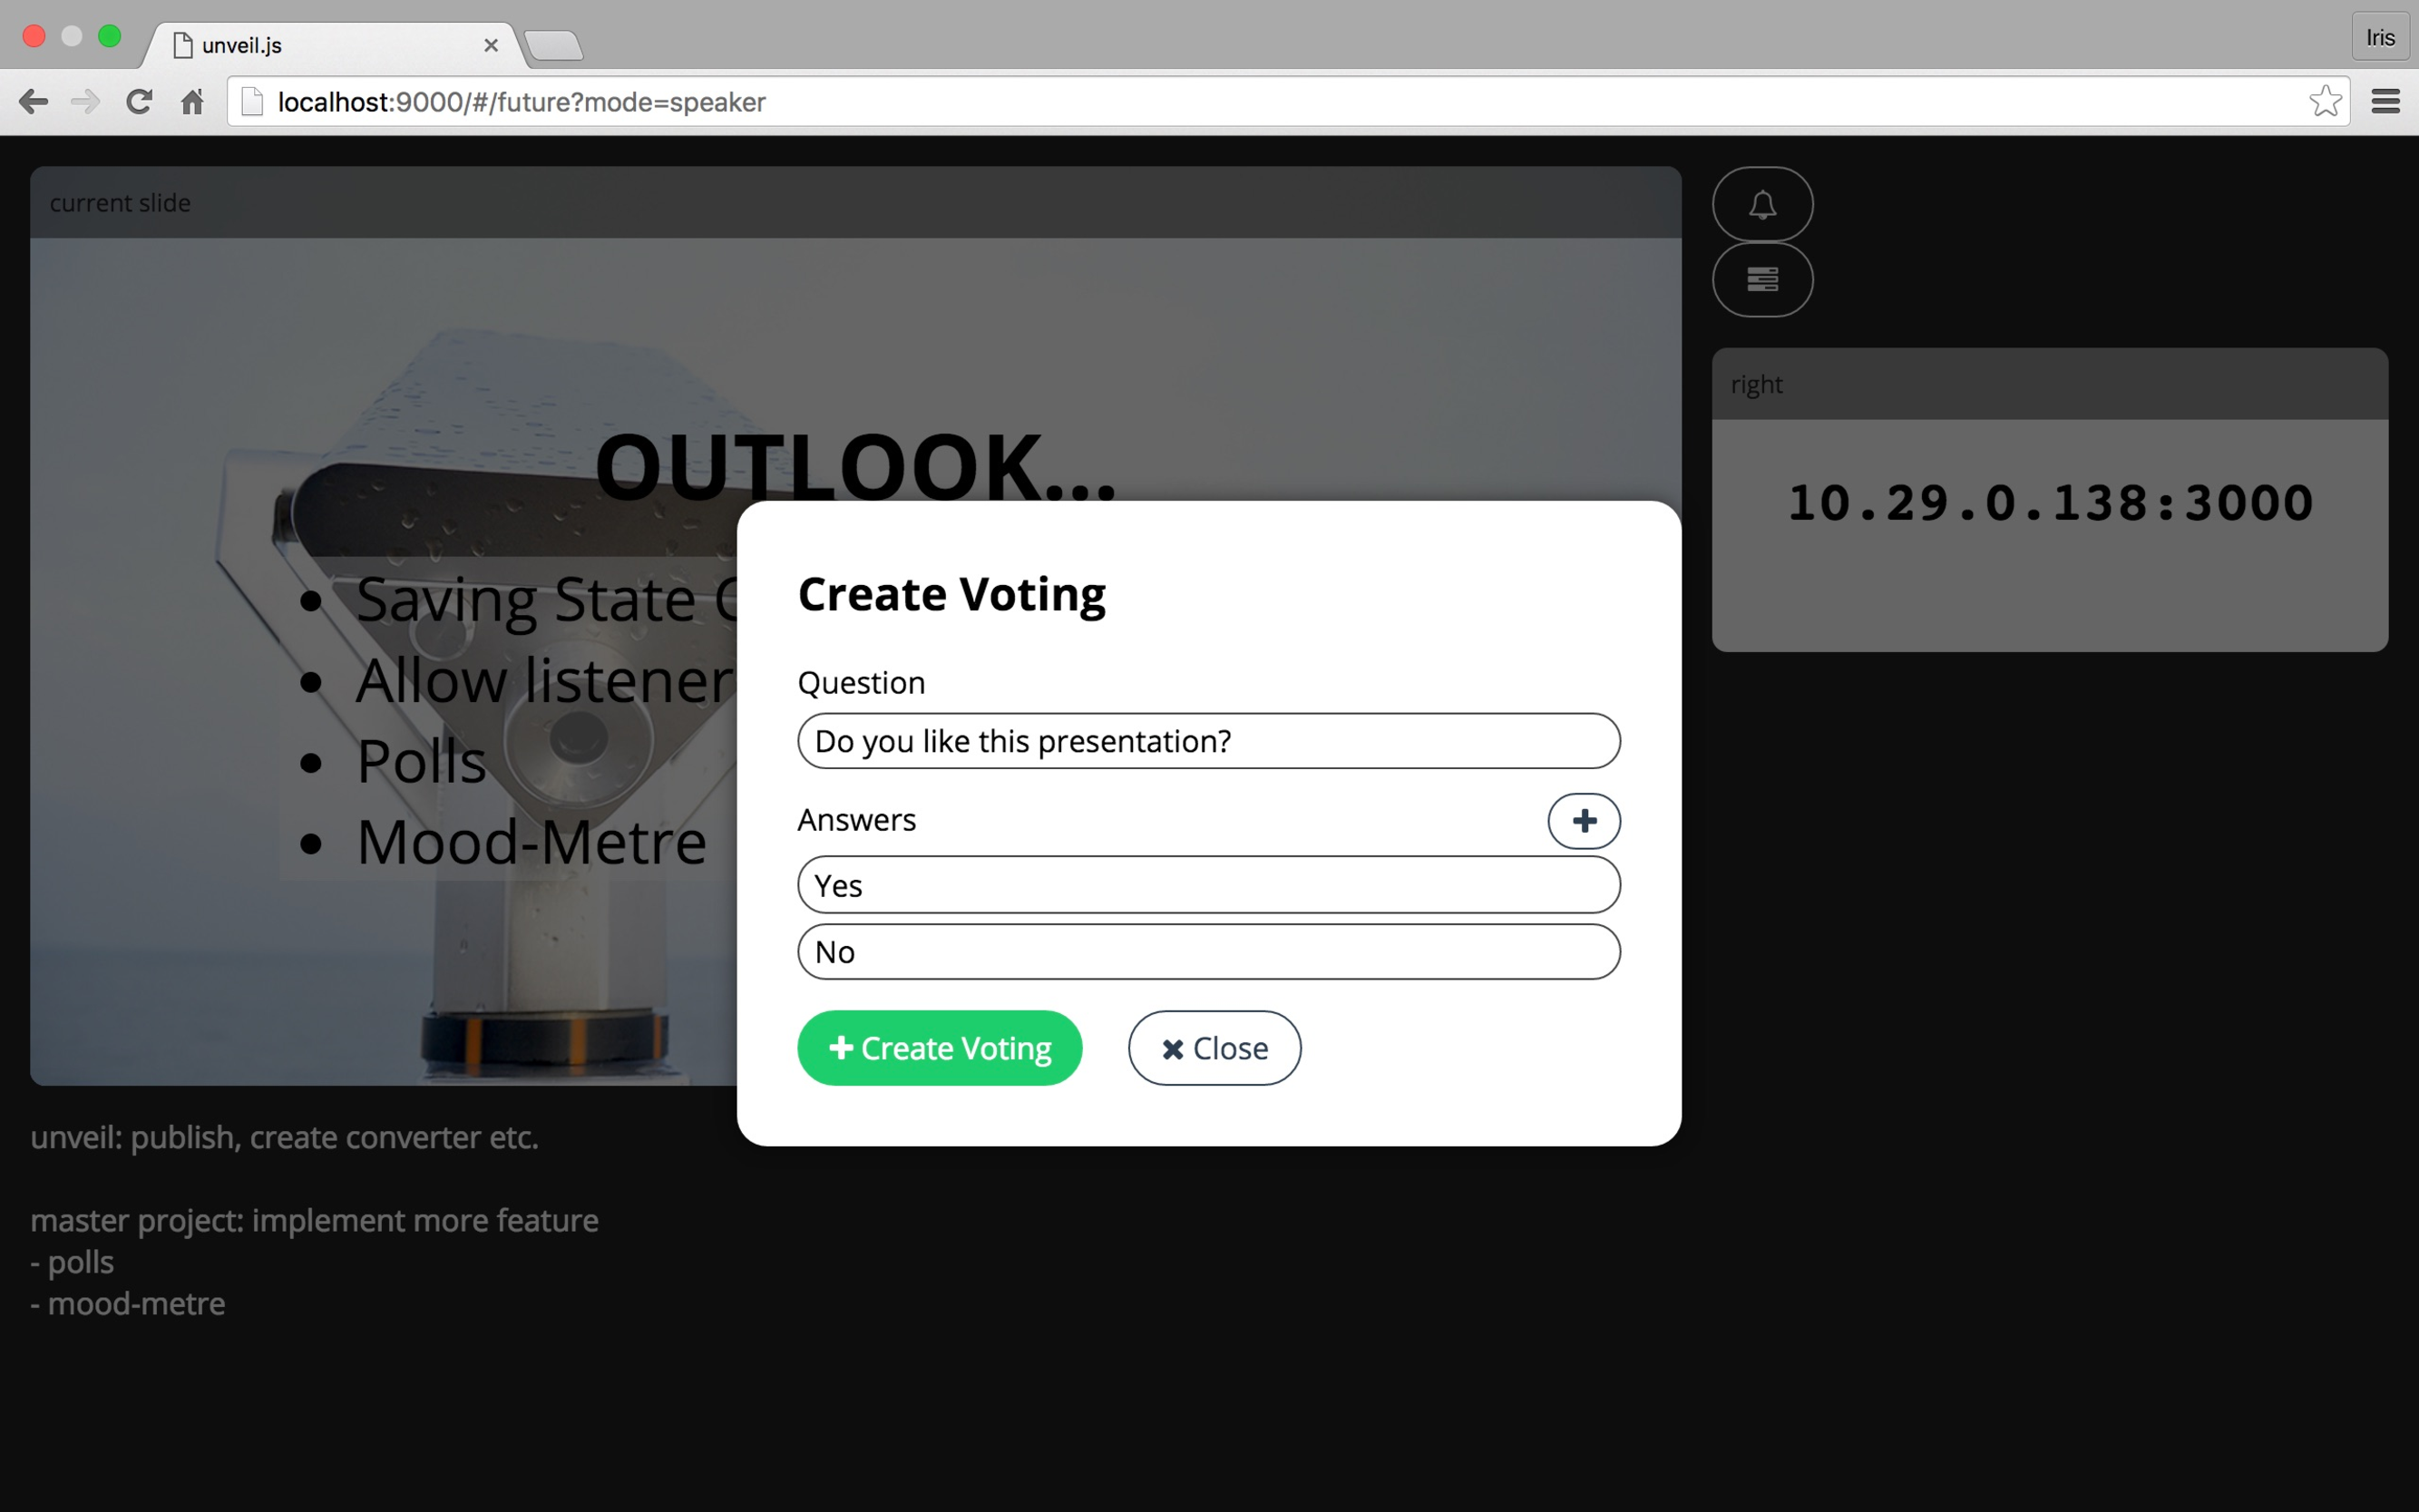
\includegraphics[width=.65\textwidth]{voting-creation-screenshot}
\caption{Screenshot of the desktop speaker mode, creating a new voting, on-the-fly, during a presentation.}
\label{fig:implementation-interactive-voting}
\end{figure}

The main presentational component involved in the voting process is \texttt{Voting}, which keeps track of the current voting scores and has a \texttt{Question} and a number of \texttt{Answer} components as children (see program \ref{prog:implementation-interactive-structure}). \texttt{Voting} also remembers if an audience member has already voted and if so, displays \texttt{Result} components. In speaker and presenter mode only these results are shown.

\begin{program}
\caption{Example code for preparing a slide with voting.}
\label{prog:implementation-interactive-structure}
\begin{JsCode}
<Voting name="like">
  <Question>Do you like these slides?</Question>
  <Answer value="yes">Yes</Answer>
  <Answer value="no">No</Answer>
</Voting>
\end{JsCode}
\end{program}

The audience can start voting as soon as the speaker navigates to the slide with the voting, until then the vote button is disabled. Once the voting has started, the possibility for all audience members to navigate to a different slide is disabled. This happens in the \texttt{VotingNavigatableSetter}, which is only installed for default mode. The voting start event, as well as the voting end event are broadcast by the \texttt{VotingController}, which checks the speaker's current slide for the occurence of a \texttt{Voting}.

Once the voting has started, internally, the \texttt{Voting} component remembers which answer the user has clicked in the \texttt{answer} state variable. Once the submit button is pressed, a \texttt{state/slide/voting:answer} event is fired and broadcast to all clients, which update their internal voting results.
Because the results of the voting should be available throughout the whole presentation and not be reset when leaving the slide, \texttt{Voting} also handles the communication with local storage, to store current results.

\section{Server}
\label{sec:implementation-server}
% shortly talk about server and how any server could really be used for this.
As shortly outlined before, the focus of this project was never the server, but instead the client. For this reason the server was kept as lightweight and dumb as possible, only handling the most important communication. In reality, it acts as a proxy and broadcaster between the clients and serves the JavaScript and HTML files.

The server developed for the project presentation of the Interactive Media course IM690 runs on Node.js, using Express\footnote{\url{http://expressjs.com/}} as a framework. To emphasise how low the requirements for such a server are, a working example implementation can be found in program \ref{prog:implementation-server-code}. Additionally to this code, the server in the unveil-client-server repository also includes a \texttt{lastState} variable, in which the last navigation state is stored. Every time a new client connects, this state is then emitted with a \texttt{state:initial} event. Moreover, socket.io does not currently support wildcards in events, which is why it was necessary to add the code snippet discussed in \cite{socket-io-wildcards}.

\begin{program}
\caption{Very simple possible implementation of a server running the thesis project with Node.js and Express. \cite{socket-io-wildcards} describes how wildcard support can be added to socket.io.}
\label{prog:implementation-server-code}
\begin{JsCode}
var express = require('express');
var app = express();
var server = require('http').createServer(app);
var io = require('socket.io')(server);

// directory 'client' will be served by server
app.use(express.static(__dirname + '/../client/'));

// setting up of socket io
io.on('connection', function(socket) {
  socket.on('*', function(event, data) {
    io.emit(event, data);
  });
});

server.listen(9000, function () {
  console.log('Unveil server listening on port 9000!');
});
\end{JsCode}
\end{program}

\section{Example Application}
\label{sec:implementation-client}
% how is everything defined? what has to be included?
% what are the steps of building an application with unveil?
% how are the slides defined? how are they styled? what about the modes?

To conclude this chapter, I want to show how all the discussed libraries in the end can be put together to a presentation. The whole presentation can be found in the unveil-client-server repository.

The first step to use unveil.js and its extensions is to start a new project, require the necessary npm packages and set up an \texttt{index.html} page which includes the necessary stylesheets and scripts.
The entry point for these scripts is the file \texttt{index.js}, in which the whole presentation is set up and unveil.js is configured by setting up its modes (see program \ref{prog:implementation-client-modes}). As explained before, slides are defined in HTML using the components unveil.js and its extensions provide. An example of this is shown in program \ref{prog:implementation-client-presentation}.

\begin{program}
\caption{Mode definition for setting up an unveil.js presentation. Speaker and projector modes are omitted to keep the example short but follow the same pattern as the default mode.}
\label{prog:implementation-client-modes}
\begin{JsCode}
const modes = {
  default: {
    controls : [
      KeyControls, TouchControls, UIControls,
      NavigationReceiver,
      MediaSender, MediaReceiver,
      VotingNavigatableSetter, VotingReceiver
    ],
    presenter: Presenter
  },
  speaker: {...},
  projector: {...}
};
\end{JsCode}
\end{program}

\begin{program}
\caption{Creation of presentation using modes from program \ref{prog:implementation-client-modes}. Sets up two slides as an example. The DOM will be attached to the element of id \texttt{unveil} in the base HTML document.}
\label{prog:implementation-client-presentation}
\begin{JsCode}
ReactDOM.render((
  <UnveilApp modes={modes}>
    <Slide name="start">
      <h1>Unveil</h1>
      <h2>a meta presentation</h2>
    </Slide>
    <Slide name="problem">
      <img src="./img/problem.png" />
      <Notes>someone always wanted to show something from their device</Notes>
    </Slide>
    ...
  </UnveilApp>
), document.getElementById('unveil'));
\end{JsCode}
\end{program}

The styling of the presentation is handled by CSS. The \texttt{Slide} component automatically adds the name of a slide as its id, allowing to efficiently style slide by slide, as well as applying styles for all slides at once using the \texttt{.slide} class. Program \ref{prog:implementation-client-styles} shows an example of how to style slides.

\begin{program}
\caption{Example styling for slides using Sass. In this particular piece of code, the font family of all slides is set and a background image is added to the start slide.}
\label{prog:implementation-client-styles}
\begin{CssCode}
  .slide
    font-family: 'Open Sans'
  #start
    background-image: url('../img/explore.jpg')
\end{CssCode}
\end{program}
\chapter{Usage of Resulting Libraries}
\label{cha:usage}

The functionality of the created libraries should now be clear, but one question remains: how can this code be used in a presentation? This chapter will go into details of how to set up an unveil presentation (section \ref{sec:usage-setup}), use the components (section \ref{sec:usage-components}) and lastly ways of customising, overwriting and extending behaviour (section \ref{sec:usage-customisation}). The code-examples of this chapter are based on \cite{unveil-client-server}.

\section{Setup}
\label{sec:usage-setup}
% how is everything defined? what has to be included?
% what are the steps of building an application with unveil?
% how are the slides defined? how are they styled? what about the modes?

Since the entire created code is available on npm, the first step in setting up an unveil presentation is to require the necessary libraries \texttt{unveil}, \texttt{unveil-network-sync} and \texttt{unveil-interactive}. In the entry point of the presentation (usually \texttt{index.html}), all bundled JavaScript and CSS-files are included and an HTML document is created which offers a tag that can be used to render the presentation (e.g. a \texttt{div} with the class \texttt{unveil}). For lower the page loading time \cite{yahoo-speeding-up-website}, script tags should generally placed in the \texttt{body} tag, usually before closing said tag.
As soon as this initial page is set up, the actual presentation can be built in an JavaScript file which should also be included here.
In this file, we will call it \texttt{index.js} from now on, all necessary libraries and components are imported:  \texttt{React}, \texttt{ReactDom}, as well as all unveil components that should be used. If any libraries which rely on the communication with the WebSocket server should be used in the presentation, the \texttt{SocketIO} singelton also has to be configured with the address of the server:
\begin{GenericCode}
import { createSocket } from 'unveil-network-sync'
createSocket('http://192.168.0.17:9000')
\end{GenericCode}

\section{Building a Presentation}
\label{sec:usage-components}

Once all libraries are imported, the actual presentation can be created. The most important component in this context is \texttt{UnveilApp}, which is imported from \texttt{unveil}. This component holds all the \texttt{Slide}s and is responsible for the configuration of the application (see section \ref{sec:usage-customisation}). Inside the \texttt{Slide} components, all content of the slide and the \texttt{Notes} are placed. Each of the slides will be rendered as common HTML and can include any number of other HTML tags and custom React components (see programm \ref{prog:usage-presentation-creation}). Although strictly-speaking not necessary, it is recommended to give slides (unique) names, since their name will be the id of the rendered HTML component and makes it possible to style components with CSS (see programm \ref{prog:usage-styling}). Additionally, if provided, unveil uses the name of the current slide as the url, allowing for text-based rather than index-based routes.

Other than that, slides can have a \texttt{left}, \texttt{right}, \texttt{up} and \texttt{down} property to allow for several paths through a presentation: All slides are provided as normal slide-sets, but the \texttt{left} and \texttt{right} attributes of the first and last slide of each path point to the previous and next slide shared by the entire presentation. \texttt{Link}s (available in the \texttt{unveil-interactive} package) can be used to access the first slide of each path. Additionally, the interactive extension also offers the components for preparing votings: \texttt{Voting}, \texttt{Question} and \texttt{Answer} (see programm \ref{prog:usage-voting}). The only necessary property for \texttt{Voting}s is the \texttt{name} attribute, which uniquely identifies the voting, as well as exactly one \texttt{Question}-child and an arbitrary number of \texttt{Answer}s.

\begin{program}
\caption{Example styling unveil slides using Sass. In this particular piece of code, the font family of all slides is set and a background image is added to the slide of name \texttt{start}.}
\label{prog:usage-styling}
\begin{CssCode}
  .slide
    font-family: 'Open Sans'
  #start
    background-image: url('../img/explore.jpg')
\end{CssCode}
\end{program}

\begin{program}
\caption{Creation of a presentation. Sets up two slides as an example. The DOM will be attached to the element of id \texttt{unveil} in the base HTML document.}
\label{prog:usage-presentation-creation}
\begin{JsCode}
ReactDOM.render((
  <UnveilApp modes={modes}>
    <Slide name="start">
      <h1>Unveil</h1>
      <h2>a meta presentation</h2>
    </Slide>
    <Slide name="intro">
      <img src="./img/problem.png" />
      <Notes>Explain initial situation</Notes>
    </Slide>
    ...
  </UnveilApp>
), document.getElementById('unveil'));
\end{JsCode}
\end{program}


\begin{program}
\caption{Creation of votings in unveil. The necessary components have to be imported from \texttt{unveil-interactive}.}
\label{prog:usage-voting}
\begin{JsCode}
<Voting name="like">
  <Question>Do you like these slides?</Question>
  <Answer value="yes">Yes</Answer>
  <Answer value="no">No</Answer>
</Voting>
\end{JsCode}
\end{program}

\section{Customisation and Extenstion}
\label{sec:usage-customisation}

\begin{program}
\caption{Mode definition for setting up an unveil.js presentation. Default (i.e. listener) and speaker modes are omitted to keep the example short, but generally follow the same pattern as the projector mode.}
\label{fig:usage-modes}
\begin{JsCode}
const modes = {
  default: {...},
  speaker: {...},
  projector: {
    controls : [
      NavigationReceiver, MediaReceiver, ReactionReceiver,
      VotingNavigatableSetter, VotingReceiver
    ],
    presenter: Presenter
  }
};
\end{JsCode}
\end{program}

Thanks to unveil's base architecture, it is possible for speakers to entirely customise the entire presentation logic. The most important step is to define the available modes and the presenter and controls which should be loaded in each of them (see figure \ref{fig:usage-modes}). Additionally to the existing controls in unveil and its current extensions, new (presentation) logic can be added by defining ones own React components and assigning them to modes. To interact with the WebSocket server, \texttt{SocketIO} is available from the network synchronisation layer. Data such as the current router state or slide, and the navigator or state subject are accessible through \texttt{UnveilApp}'s context. For examples of existing controls and presenters, the reader is adviced to refer to the implementation of the components discussed in chapter \ref{cha:implementation} \cite{unveil-fork, unveil-network-sync, unveil-interactive}.

Moreover, the \texttt{Router} and \texttt{Navigator} can also be entirely replaced by providing ones own functionality as \texttt{router} and \texttt{navigator} properties in \texttt{UnveilApp}. They only have to follow the same interface as the default implementations. If any additional configuration should be necessary (such as with setting the address of the WebSocket server or customising emoji), singletons or static methods of the components can be used.
\chapter{Discussion}
\label{cha:discussion}

A system such as the one developed in course of this thesis can be evaluated in many ways: the performance of the software can be quantified by measuring response times of the application, as happened in \cite{Niwa:Web-presentation-powerpoint} or \cite{Inoue:RealTimeQuestionnaire}, the usability can be assessed qualitatively through usability tests, measuring error rates and time to complete certain tasks and qualitatively using \emph{loud thinking} and interviews \cite{Reindl:automatisierte-user-interface-evaluierung}. If listeners feel more engaged and whether the perception of phone usage in a presentation has changed can also be estimated using qualitative and quantitative evaluation methods, however, valid results can only be achieved observing the usage of the presented tool over a longer period of time and involving a control group. Since this would go beyond the scope of a master thesis, we instead decided to refrain from a formal study and instead rely on the informal observation and evaluation of the system, both during and after working on the project.
Throughout the process of developing the different libraries, several presentations and meetings have been held using the resulting libraries, both in informal and formal as well as academic and business settings. This allowed for several iterations of the design, as well as the gradual introduction of more and more interactive mechanisms. Our findings and the strengths and the shortcomings of the project will be discussed in this chapter, followed by an outlook on future work.

\section{Usability}
We were pleased to see that all listeners understood the base interface of the application, both on their phones and on the laptop. We have however not had a single tablet user in any of the presentations held so far and most of the mobile phones were iPhones running Chrome or Safari. Some users experienced glitches in the navigation of the slides and could scroll within them, moreover mobile Safari seemed to have difficulties with local storage (and thus persisting voting results), on some devices. On the other hand, the concerns regarding the usage of socket.io have not come true, since the presentations were always held in networks we had control over (so corporate firewalls did not play a role).

As far as the response time of the application is concerned, with up to 30 concurrent users, no noticable declines in performance have been experienced so far and the real-time features feel instantaneous. The only current limitation to this is the transmission of base64-encoded media content through the WebSocket. Since the delay is between listener and speaker, however, the transmission time is not critical for the application to feel responsive. Another point connected to this mechanism was that some users were missing the possibility to natively share content from their phones, which was an anticipated limitation of creating a web application over a mobile one.
The sharing features have generally been accepted by users and seemed to have caused most excitement about the new technology. In our trials, however, we experienced a large amount of test-data being sent through the mechansisms, especially in the beginning of the presentation. We therefore advice others to provide one or two empty slides in the beginning of the presentation if the audience is new to the software, so the application and its functionality can be explored. Since some users mixed textual content with links in the early tests, we now separated media upload, link sharing and questions (or other text) from each other.
The reaction-system was the one implemented last, which is why we are still missing more thorough insight into how listeners use it. In informal feedback rounds about the mechanism, the usage of emoji seemed to be understood well, however, these conversations were held with digital professionals and will require further analysis.
The voting mechanism was also understood by users and no questions have yet arisen from it. To our surprise this functionality, like the possibility of having different paths through the presentation, did not seem to impress or excite users too much.

The biggest weakness of unveil for most users, was the inability for the presentation to be permanently altered. Especially in meetings and informational presentations, many listeners asked for a link to the collaboratively created presentation afterwards, some users were forced to reload the website due to cross-browser compatibility issues and lost the current state of the slides, late-comers also did not have the possibility to jump into an already altered presentation. This will make it necessary to create a more intelligent and opinionated back end in the future.

\section{Creation of Presentation}
Most of the feedback we have collected about unveil over the last months came from listeners. This has two reasons: Firstly, the creation of presentations requires knowledge and experience with front end web development technologies, secondly, we have not started promoting the resulting libraries yet, as we feel the system is not stable and mature enough to be used outside. However, external developers have provided us with their feedback regarding the syntax used for defining slide decks and seem to not have had any problems understanding the usage of the libraries, what validates our decision to choose semantically-named tags rather than HTML class names to identify different components. On the downside, we seem to have overestimated the level of knowledge necessary to create own presentations, as a few developers were not entirely familiar with the new ES6 syntax and the process of bundling JavaScript and CSS files, so an easier way of importing all necessary libraries should be provided in an example presentation.
In the long run, this product will only be able to increase its popularity if a visual editor for authoring slides, as well as a system to manage (i.e. host) them will be available. Some users also raised the question of how and if it was possible to import PowerPoint presentations, to be able to use the created mechanisms in connection with already existing software.

\section{Architecture}
Generally, it has to be said that the project is still only a prototype and does not provide the stability necessary for us to feel confident promoting the product. One particular problem we have been experiencing irregularly is the navigation getting stuck in an infinite redirect loop when having more than one presenter at a given time, who try to navigate simultaneously. 
Although the chosen architecture allows for a lot of flexibility and freedom for developer and in that sense fulfils the criteria impress.js and reveal.js did not, we have lately discovered more powerful, streamlined and widespread patterns when working with React. Since we had no experience with React prior to the start of the development, best practices oftentimes only became apparent throughout the project and through the work on and with other React applications. To make the libraries yet easier to use and extend and more easily debuggable, future iterations of unveil will be based on redux \cite{redux}. This will make it easier to decouple components from each other through the introduction of a state container.
\chapter{Conclusions}
\label{cha:conclusion}

In this thesis, we present \emph{unveil}: an extensible JavaScript presentation eco\-system with a multitude of interactive mechanisms, aiming to make presentations more engaging, memorable and collaborative. At its core stand four React libraries, connecting presenters, listeners and projectors through a WebSocket server, making it possible for both audience and speakers to alter $2$-dimensional slide-sets in real time.
Different types of presentations were analysed to find their weaknesses and establish ways of enhancing the presentation experience: To make it easier to esitmate the listeners' level of knowledge, a real-time voting mechanism was implemented, allowing for both prepared polls and ones created on-the-fly during the presentation. Furthermore, the audience can instantaneously react to slides via emoji, giving the speaker an impression of the current mood. To account for individual learning-pace and late-comers, members of the audience can moreover browse and follow the slides on their personal devices as well as send questions to the presenter.
These questions, along with other multi-media content, such as pictures and links to websites and youtube videos, can then be embedded into the presentation as new main or sub-slides, effectively enabeling the audience to truely shape he presentation using nothing but the mobile devices they carry on them. This holds the potential of engaging listeners in the presentation, steering it towards certain topics, connecting members of the audience with each other and the speaker and adding related content for further reference.

Despite making presentations more memorable for the audience, this approach poses new challenges and requires more flexibility from the speaker, which is why all realised mechanisms can easily be activated an deactivated. Since the created libraries were generally designed for other developers to re-use, modify and extend, we moreover offer ways of tailoring and configuring every last detail, from the routing logic over the emoji displayed to the mechanisms enabled for each user group (presenter, listener, projector).

Although long-term studies will be necessary to validate our approach and verify and quantify their success, initial observation and evaluation of the system showed promising results. The users understood the interface and were especially excited about the possibility of sharing their own content and thoughts with the presentation. This mechanism was particularly well-accepted during informal meetings, were the usage organically evolved into a brain-storming like activity, involving all participants. The initial evaluation of our prototype also showed room for improvement, amongst others, the persistence of the created presentation and the absence of native sharing features on the phone. In future iterations of the libraries, the stability and testability of the platform will be improved as well as offering a way of permanently altering the presentation.
Moreover, a graphical user interface for the creation of slides is desirable, effectively opening interactive presentations to non-developers. The trials also gave way to ideas for future projects, most notably the combination of these interactive mechanisms with existing presentation software, with canvas-based ones being of special interest.

% Hier könnte man erwähnen dass das sharen mittels handy übers menü doch irgendwie besser wäre, aber den Nachteil hat dass man sich die app herunterladen muss.
% erwähnen: Könnte evtl. auch für remote presentationen verwendet werden!
% erwähnen: evtl. andere typen von Charts (Pie etc.) wie erwähnt in Electronic voting on the fly
% auszerdem: von power point exportieren wäre riesen Vorteil für Author!
% Wie wärs mit: Hinweis darauf, dass es wichtig ist die richtigen Mechanismen für die richtige Präsentation zu wählen um death by technology zu vermeiden (referenz zu \cite{Wacker:PresenterExperience}, dass failing technology reason #1 ist sich unwohl zu fühlen!). Mechanismen sollen nicht menschliche Kommunikation ersetzen sonder unterstützen und sind nicht immer nötig und mit Vorsicht zu genieszen
% Application for workshop environment (wie am Anfang besprochen! Großgruppe => Kleingruppe => Großgruppe)
% Sicherheitsconcerns nicht beachtet 
% Mehr tests benötigt, aber erste tests zeigen: Anfangsslide zum Austoben einbauen, App wird gut angenommen auch wenn Funktionen in Meetings mehr genutzt werden als in anderen Präsentationen
% Speichern der Resultate auf Implementierungsseite noch benötigt

%%%----------------------------------------------------------
%%%Anhang
\appendix
\chapter{DVD  Contents}
\label{app:cdrom}

\section{General}

\begin{FileList}{/}
\fitem{_DaBa.pdf} Master Thesis
\fitem{questionnaires.pdf} User Study Questionnaires
\fitem{questionnaires.xlsx} User Study Results
\end{FileList}

\section{Copies of Online References}

\begin{FileList}{/references/}
\fitem{about-iclicker.pdf} About i>clicker \cite{iclicker}.
\fitem{babel-users.pdf} See who's using Babel \cite{babel-users}.
\fitem{bing-emoji.pdf} Do You Speak Emoji? Bing Does \cite{Bing:Emoji}.
\fitem{creative-bloq-hover.pdf} Hover is dead, long live hover \cite{hover}.
\fitem{cu-clickers-faq.pdf} CUClickers / i>clickers - FAQ \cite{cuclickers:faq}.
\fitem{ecma-262.pdf} ECMAScript 2015 Language Specification \cite{ecma2015}.
\fitem{facebook-reactions.pdf} Reactions Now Available Globally \cite{Facebook:Reactions}.
\fitem{github-reactions.pdf} Add Reactions to Pull Requests, Issues, and Comments \cite{Github:Reactions}.
\fitem{google-emoji.pdf} Google now also allows you to search using emoji characters \cite{Google:Emoji}.
\fitem{instagram-emoji.pdf} Emojineering Part 1: Machine Learning for Emoji Trends \cite{Instagramm:Emoji}.
\fitem{jsx-specification.pdf} Draft: JSX Specification \cite{jsx}.
\fitem{mozilla-file-api.pdf} Using files from web applications \cite{file-api}.
\fitem{npm-babel.pdf} npm's babel package page \cite{npm-babel}.
\fitem{prezi-presentations.pdf} The Science of Effective Presentations \cite{prezi-science}.
\fitem{react-benchmarks.pdf} More Benchmarks: Virtual DOM vs Angular 1 \& 2 vs Mithril.js vs cito.js vs The Rest \cite{react-benchmarks}.
\fitem{sm-es6.pdf} ECMAScript 6 (ES6): What's New In The Next Version Of JavaScript \cite{es6}.
\fitem{so-developer-survey.pdf} 2015 Developer Survey \cite{stackoverflow-developer-survey}.
\fitem{socketio-problems.pdf} Why We Ditched Socket.IO \cite{socketio-problems}.
\fitem{socketio-wildcards.pdf} Answer to Stack Overflow Question ``Socket.io Client: respond to all events with one handler?'' \cite{socket-io-wildcards}.
\fitem{yahoo-performance.pdf} Best Practices for Speeding Up Your Web Site \cite{yahoo-speeding-up-website}.
\end{FileList}

\section{Graphics}

\begin{FileList}{/graphics/}
\fitem{screenshots/*} Screenshots of unveil %
\fitem{wireframes/*.pdf}  Annotated Wireframes%
\fitem{wireframes/*.png} Original Balsamiq Wireframes%
\fitem{*.jpg, *.png} Original Raster Graphics %
\fitem{*.pdf} Original Vector Graphics %
\fitem{*.sketch} Original Sketch Files %
\fitem{*.ai} Original Illustrations %
\end{FileList}



%%%----------------------------------------------------------
\MakeBibliography
%%%----------------------------------------------------------

%%%Messbox zur Druckkontrolle
\chapter*{Messbox zur Druckkontrolle}



\begin{center}
{\Large --- Druckgröße kontrollieren! ---}

\bigskip

\Messbox{100}{50} % Angabe der Breite/Hoehe in mm

\bigskip

{\Large --- Diese Seite nach dem Druck entfernen! ---}

\end{center}



\end{document}
